% Options for packages loaded elsewhere
\PassOptionsToPackage{unicode}{hyperref}
\PassOptionsToPackage{hyphens}{url}
%
\documentclass[
]{book}
\usepackage{lmodern}
\usepackage{amsmath}
\usepackage{ifxetex,ifluatex}
\ifnum 0\ifxetex 1\fi\ifluatex 1\fi=0 % if pdftex
  \usepackage[T1]{fontenc}
  \usepackage[utf8]{inputenc}
  \usepackage{textcomp} % provide euro and other symbols
  \usepackage{amssymb}
\else % if luatex or xetex
  \usepackage{unicode-math}
  \defaultfontfeatures{Scale=MatchLowercase}
  \defaultfontfeatures[\rmfamily]{Ligatures=TeX,Scale=1}
\fi
% Use upquote if available, for straight quotes in verbatim environments
\IfFileExists{upquote.sty}{\usepackage{upquote}}{}
\IfFileExists{microtype.sty}{% use microtype if available
  \usepackage[]{microtype}
  \UseMicrotypeSet[protrusion]{basicmath} % disable protrusion for tt fonts
}{}
\makeatletter
\@ifundefined{KOMAClassName}{% if non-KOMA class
  \IfFileExists{parskip.sty}{%
    \usepackage{parskip}
  }{% else
    \setlength{\parindent}{0pt}
    \setlength{\parskip}{6pt plus 2pt minus 1pt}}
}{% if KOMA class
  \KOMAoptions{parskip=half}}
\makeatother
\usepackage{xcolor}
\IfFileExists{xurl.sty}{\usepackage{xurl}}{} % add URL line breaks if available
\IfFileExists{bookmark.sty}{\usepackage{bookmark}}{\usepackage{hyperref}}
\hypersetup{
  pdftitle={회귀모형 이론과 계산},
  pdfauthor={서울시립대학교 통계학과 이용희},
  hidelinks,
  pdfcreator={LaTeX via pandoc}}
\urlstyle{same} % disable monospaced font for URLs
\usepackage{color}
\usepackage{fancyvrb}
\newcommand{\VerbBar}{|}
\newcommand{\VERB}{\Verb[commandchars=\\\{\}]}
\DefineVerbatimEnvironment{Highlighting}{Verbatim}{commandchars=\\\{\}}
% Add ',fontsize=\small' for more characters per line
\usepackage{framed}
\definecolor{shadecolor}{RGB}{248,248,248}
\newenvironment{Shaded}{\begin{snugshade}}{\end{snugshade}}
\newcommand{\AlertTok}[1]{\textcolor[rgb]{0.94,0.16,0.16}{#1}}
\newcommand{\AnnotationTok}[1]{\textcolor[rgb]{0.56,0.35,0.01}{\textbf{\textit{#1}}}}
\newcommand{\AttributeTok}[1]{\textcolor[rgb]{0.77,0.63,0.00}{#1}}
\newcommand{\BaseNTok}[1]{\textcolor[rgb]{0.00,0.00,0.81}{#1}}
\newcommand{\BuiltInTok}[1]{#1}
\newcommand{\CharTok}[1]{\textcolor[rgb]{0.31,0.60,0.02}{#1}}
\newcommand{\CommentTok}[1]{\textcolor[rgb]{0.56,0.35,0.01}{\textit{#1}}}
\newcommand{\CommentVarTok}[1]{\textcolor[rgb]{0.56,0.35,0.01}{\textbf{\textit{#1}}}}
\newcommand{\ConstantTok}[1]{\textcolor[rgb]{0.00,0.00,0.00}{#1}}
\newcommand{\ControlFlowTok}[1]{\textcolor[rgb]{0.13,0.29,0.53}{\textbf{#1}}}
\newcommand{\DataTypeTok}[1]{\textcolor[rgb]{0.13,0.29,0.53}{#1}}
\newcommand{\DecValTok}[1]{\textcolor[rgb]{0.00,0.00,0.81}{#1}}
\newcommand{\DocumentationTok}[1]{\textcolor[rgb]{0.56,0.35,0.01}{\textbf{\textit{#1}}}}
\newcommand{\ErrorTok}[1]{\textcolor[rgb]{0.64,0.00,0.00}{\textbf{#1}}}
\newcommand{\ExtensionTok}[1]{#1}
\newcommand{\FloatTok}[1]{\textcolor[rgb]{0.00,0.00,0.81}{#1}}
\newcommand{\FunctionTok}[1]{\textcolor[rgb]{0.00,0.00,0.00}{#1}}
\newcommand{\ImportTok}[1]{#1}
\newcommand{\InformationTok}[1]{\textcolor[rgb]{0.56,0.35,0.01}{\textbf{\textit{#1}}}}
\newcommand{\KeywordTok}[1]{\textcolor[rgb]{0.13,0.29,0.53}{\textbf{#1}}}
\newcommand{\NormalTok}[1]{#1}
\newcommand{\OperatorTok}[1]{\textcolor[rgb]{0.81,0.36,0.00}{\textbf{#1}}}
\newcommand{\OtherTok}[1]{\textcolor[rgb]{0.56,0.35,0.01}{#1}}
\newcommand{\PreprocessorTok}[1]{\textcolor[rgb]{0.56,0.35,0.01}{\textit{#1}}}
\newcommand{\RegionMarkerTok}[1]{#1}
\newcommand{\SpecialCharTok}[1]{\textcolor[rgb]{0.00,0.00,0.00}{#1}}
\newcommand{\SpecialStringTok}[1]{\textcolor[rgb]{0.31,0.60,0.02}{#1}}
\newcommand{\StringTok}[1]{\textcolor[rgb]{0.31,0.60,0.02}{#1}}
\newcommand{\VariableTok}[1]{\textcolor[rgb]{0.00,0.00,0.00}{#1}}
\newcommand{\VerbatimStringTok}[1]{\textcolor[rgb]{0.31,0.60,0.02}{#1}}
\newcommand{\WarningTok}[1]{\textcolor[rgb]{0.56,0.35,0.01}{\textbf{\textit{#1}}}}
\usepackage{longtable,booktabs}
\usepackage{calc} % for calculating minipage widths
% Correct order of tables after \paragraph or \subparagraph
\usepackage{etoolbox}
\makeatletter
\patchcmd\longtable{\par}{\if@noskipsec\mbox{}\fi\par}{}{}
\makeatother
% Allow footnotes in longtable head/foot
\IfFileExists{footnotehyper.sty}{\usepackage{footnotehyper}}{\usepackage{footnote}}
\makesavenoteenv{longtable}
\usepackage{graphicx}
\makeatletter
\def\maxwidth{\ifdim\Gin@nat@width>\linewidth\linewidth\else\Gin@nat@width\fi}
\def\maxheight{\ifdim\Gin@nat@height>\textheight\textheight\else\Gin@nat@height\fi}
\makeatother
% Scale images if necessary, so that they will not overflow the page
% margins by default, and it is still possible to overwrite the defaults
% using explicit options in \includegraphics[width, height, ...]{}
\setkeys{Gin}{width=\maxwidth,height=\maxheight,keepaspectratio}
% Set default figure placement to htbp
\makeatletter
\def\fps@figure{htbp}
\makeatother
\setlength{\emergencystretch}{3em} % prevent overfull lines
\providecommand{\tightlist}{%
  \setlength{\itemsep}{0pt}\setlength{\parskip}{0pt}}
\setcounter{secnumdepth}{5}
%----- my options----------------
\usepackage[hangul]{kotex}
\usepackage{bm}
\usepackage{fullpage}

\newcommand{\pardiff}[2]{\frac{\partial #1}{\partial #2 }}
\newcommand{\pardiffl}[2]{{\partial #1}/{\partial #2 }}
\newcommand{\pardiffd}[2]{\frac{\partial^2 #1}{\partial #2^t \partial #2 }}
\newcommand{\pardiffdd}[3]{\frac{\partial^2 #1}{\partial #2 \partial #3 }}
\newcommand{\norm}[1]{\left\lVert#1\right\rVert}
\newcommand{\hatmat}{\bm X ({\bm X}^t {\bm X} )^{-1} {\bm X}^t}
\newcommand{\hatmatt}[1]{\bm X_{#1} ({\bm X}_{#1}^t {\bm X}_{#1})^{-1} {\bm X}_{#1}^t}

%--------- from bookdown.org --------------

\usepackage{booktabs}


\usepackage{framed,color}
\definecolor{shadecolor}{RGB}{248,248,248}

\renewcommand{\textfraction}{0.05}
\renewcommand{\topfraction}{0.8}
\renewcommand{\bottomfraction}{0.8}
\renewcommand{\floatpagefraction}{0.75}

\renewenvironment{quote}{\begin{VF}}{\end{VF}}
\let\oldhref\href
\renewcommand{\href}[2]{#2\footnote{\url{#1}}}

\makeatletter
\newenvironment{kframe}{%
\medskip{}
\setlength{\fboxsep}{.8em}
 \def\at@end@of@kframe{}%
 \ifinner\ifhmode%
  \def\at@end@of@kframe{\end{minipage}}%
  \begin{minipage}{\columnwidth}%
 \fi\fi%
 \def\FrameCommand##1{\hskip\@totalleftmargin \hskip-\fboxsep
 \colorbox{shadecolor}{##1}\hskip-\fboxsep
     % There is no \\@totalrightmargin, so:
     \hskip-\linewidth \hskip-\@totalleftmargin \hskip\columnwidth}%
 \MakeFramed {\advance\hsize-\width
   \@totalleftmargin\z@ \linewidth\hsize
   \@setminipage}}%
 {\par\unskip\endMakeFramed%
 \at@end@of@kframe}
\makeatother

\makeatletter

\@ifundefined{Shaded}{
}{\renewenvironment{Shaded}{\begin{kframe}}{\end{kframe}}}
\makeatother

\newenvironment{rmdblock}[1]
  {
  \begin{itemize}
  \renewcommand{\labelitemi}{
    \raisebox{-.7\height}[0pt][0pt]{
      {\setkeys{Gin}{width=3em,keepaspectratio}\includegraphics{images/#1}}
    }
  }
  \setlength{\fboxsep}{1em}
  \begin{kframe}
  \item
  }
  {
  \end{kframe}
  \end{itemize}
  }
  
\newenvironment{rmdnote}
  {\begin{rmdblock}{note}}
  {\end{rmdblock}}
  
\newenvironment{rmdcaution}
  {\begin{rmdblock}{caution}}
  {\end{rmdblock}}
  
\newenvironment{rmdimportant}
  {\begin{rmdblock}{important}}
  {\end{rmdblock}}
  
\newenvironment{rmdtip}
  {\begin{rmdblock}{tip}}
  {\end{rmdblock}}
  
\newenvironment{rmdwarning}
  {\begin{rmdblock}{warning}}
  {\end{rmdblock}}
  


\usepackage{makeidx}
\makeindex

\urlstyle{tt}

\usepackage{amsthm}
\makeatletter
 \def\thm@space@setup{%
   \thm@preskip=8pt plus 2pt minus 4pt
   \thm@postskip=\thm@preskip
}
\makeatother

\frontmatter
\usepackage{booktabs}
\usepackage{longtable}
\usepackage{array}
\usepackage{multirow}
\usepackage{wrapfig}
\usepackage{float}
\usepackage{colortbl}
\usepackage{pdflscape}
\usepackage{tabu}
\usepackage{threeparttable}
\usepackage{threeparttablex}
\usepackage[normalem]{ulem}
\usepackage{makecell}
\usepackage{xcolor}
\ifluatex
  \usepackage{selnolig}  % disable illegal ligatures
\fi
\usepackage[]{natbib}
\bibliographystyle{apalike}

\title{회귀모형 이론과 계산}
\author{서울시립대학교 통계학과 이용희}
\date{2021-05-11}

\usepackage{amsthm}
\newtheorem{theorem}{Theorem}[chapter]
\newtheorem{lemma}{Lemma}[chapter]
\newtheorem{corollary}{Corollary}[chapter]
\newtheorem{proposition}{Proposition}[chapter]
\newtheorem{conjecture}{Conjecture}[chapter]
\theoremstyle{definition}
\newtheorem{definition}{정의}[chapter]
\theoremstyle{definition}
\newtheorem{example}{예제}[chapter]
\theoremstyle{definition}
\newtheorem{exercise}{Exercise}[chapter]
\theoremstyle{definition}
\newtheorem{hypothesis}{Hypothesis}[chapter]
\theoremstyle{remark}
\newtheorem*{remark}{참고}
\newtheorem*{solution}{Solution}
\begin{document}
\maketitle

{
\setcounter{tocdepth}{1}
\tableofcontents
}
\hypertarget{preface}{%
\chapter*{Preface}\label{preface}}


이 책은 회귀분석에 대한 교재이며 일반 선형모형에 대한 이론을 최대 가능도 추정법의 관점에서 설명합니다. 또한 실제 예제를 통한 실습, 모형을 적합하는 계산방법과 연관된 행렬이론에 대하여 다루고자 합니다.

\begin{rmdimportant}
이 책에서 사용된 기호, 표기법, 프로그램의 규칙과 쓰임은 다음과 같습니다.

\begin{itemize}
\tightlist
\item
  스칼라(scalar)와 일변량 확률변수는 일반적으로 보통 글씨체의 소문자로 표기한다. 특별한 이유가 있는 경우 대문자로 표시할 것이다.
\item
  벡터, 행렬, 다변량 확률벡터는 굵은 글씨체로 표기한다.
\item
  통계 프로그램은 \texttt{R}을 이용하였다. 각 예제에 사용된 \texttt{R} 프로그램은 코드 상자를 열면 나타난다.
\item
  통계 프로그램은 \texttt{R}에 대한 기초는 저자의 홈페이지에 있는 \href{https://ilovedata.github.io/computing/}{안내 사이트}에서 먼저 학습할 것을 권장한다.
\end{itemize}
\end{rmdimportant}

이 교과서에서 이용하는 R 패키지는 다음과 같다.

\begin{verbatim}
library(ggplot2)
library(tidyr)
library(dplyr)
library(kableExtra)
library(agricolae)
library(emmeans)
\end{verbatim}

\mainmatter

\hypertarget{lse}{%
\chapter{선형회귀 모형과 추정}\label{lse}}

\hypertarget{uxb2e8uxc21c-uxd68cuxadc0uxbaa8uxd615}{%
\section{단순 회귀모형}\label{uxb2e8uxc21c-uxd68cuxadc0uxbaa8uxd615}}

\begin{example}[자동차의 제동거리]
\protect\hypertarget{exm:unnamed-chunk-4}{}{\label{exm:unnamed-chunk-4} \iffalse (자동차의 제동거리) \fi{} }
자동차가 달리는 속도(\texttt{speed},단위는 mph; mile per hour)와 제동거리(\texttt{dist}, 단위는 ft;feet)의 관계를 알아보기 위하여 50대의 자동차로 실험한 결과의 자료 \texttt{cars} 는 다음과 같다(처음 10개의 자료만 보여준다). 자료는 \texttt{R} 의 \texttt{data.frame} 형식으로 저장되어 있다.
\end{example}

\begin{Shaded}
\begin{Highlighting}[]
\NormalTok{cars }\SpecialCharTok{\%\textgreater{}\%} \FunctionTok{head}\NormalTok{(}\AttributeTok{n=}\DecValTok{10}\NormalTok{) }\SpecialCharTok{\%\textgreater{}\%} \FunctionTok{kbl}\NormalTok{() }\SpecialCharTok{\%\textgreater{}\%}  \FunctionTok{kable\_paper}\NormalTok{(}\StringTok{"hover"}\NormalTok{, }\AttributeTok{full\_width =}\NormalTok{ F)}
\end{Highlighting}
\end{Shaded}

\begin{table}
\centering
\begin{tabular}[t]{r|r}
\hline
speed & dist\\
\hline
4 & 2\\
\hline
4 & 10\\
\hline
7 & 4\\
\hline
7 & 22\\
\hline
8 & 16\\
\hline
9 & 10\\
\hline
10 & 18\\
\hline
10 & 26\\
\hline
10 & 34\\
\hline
11 & 17\\
\hline
\end{tabular}
\end{table}

자동차의 속도와 제동거리에 대한 산포도는 아래와 같다.

\begin{Shaded}
\begin{Highlighting}[]
\FunctionTok{ggplot}\NormalTok{(cars, }\FunctionTok{aes}\NormalTok{(}\AttributeTok{x=}\NormalTok{speed, }\AttributeTok{y=}\NormalTok{dist)) }\SpecialCharTok{+} \FunctionTok{geom\_point}\NormalTok{() }\SpecialCharTok{+} \FunctionTok{labs}\NormalTok{(}\AttributeTok{x =} \StringTok{"속도"}\NormalTok{, }\AttributeTok{y =} \StringTok{"거리"}\NormalTok{)}
\end{Highlighting}
\end{Shaded}

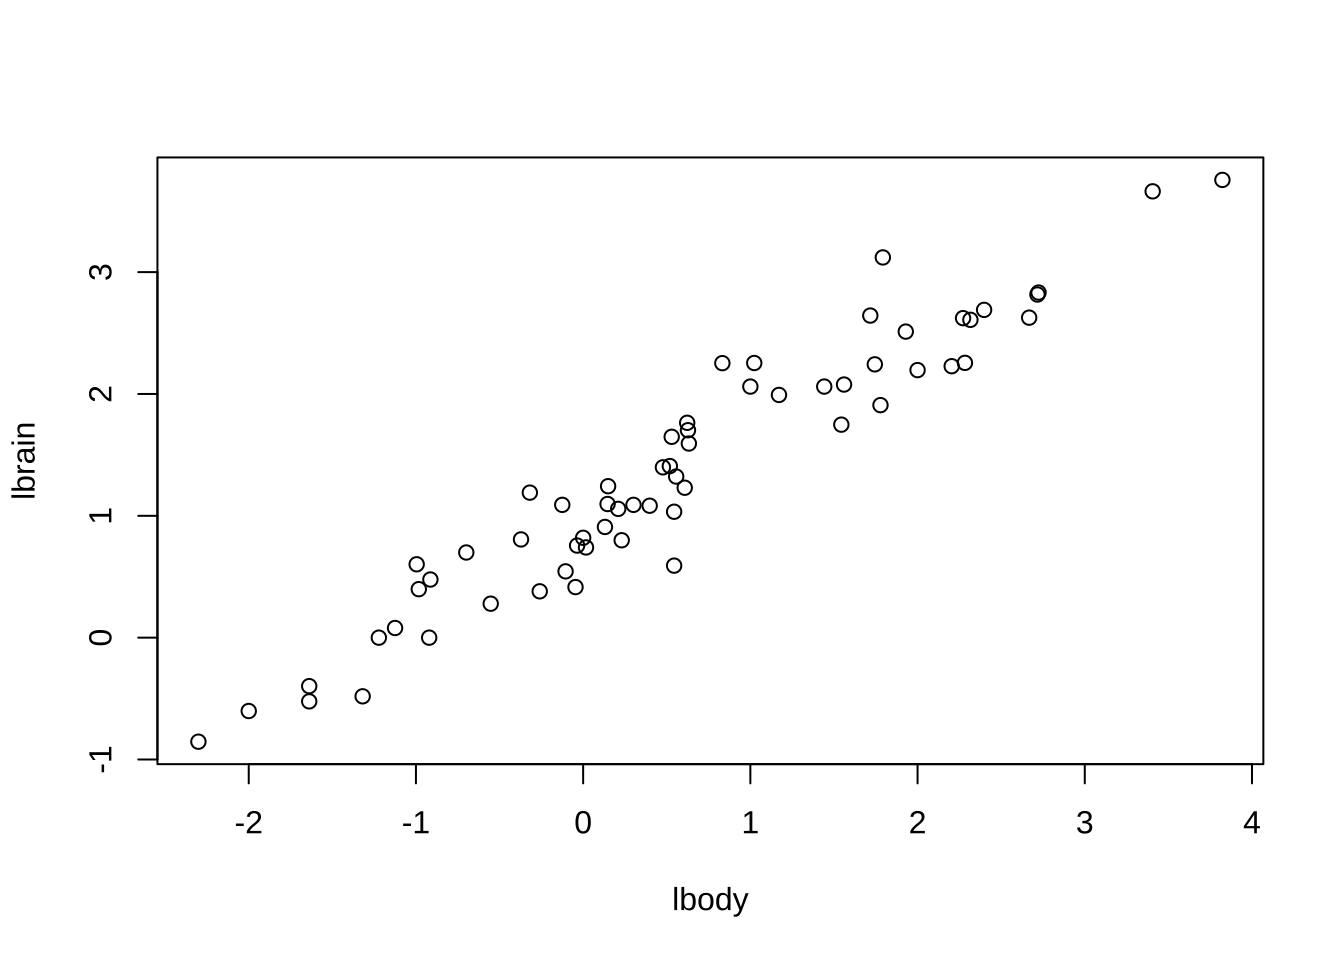
\includegraphics{lmbook_files/figure-latex/unnamed-chunk-6-1.pdf}

위와 같은 자료를 이용하여 자동차의 속도가 주어졌을 경우 제동거리를
예측하려고 한다면 어떤 방법을 사용해야 할까? 회귀분석(regression
analysis)는 여러 개의 변수들의 함수적 관계를 분석하는 통계적 방법이다.
일반적으로 한 개 또는 여러 개의 설명변수들(explanatory variables)이
관심있는 반응변수(response variable)에 어떤 형태로 영향을 미치는지에
파악하고 설명변수와 반응변수의 함수 관계를 통계적으로 추론하는 것이
회귀분석의 목적이다.

위의 예제에서 자동차의 속도를 \(x\) 라고 하고 제동거리를 \(y\) 라고 하면
다음과 같은 선형식으로 자동차의 속도와 제동거리의 관계를 나타내는 것을
선형회귀식(linear regression function) 또는 선형예측식(linear
predictor)이라고 한다.

\begin{equation} 
E(y|x) = \beta_0 + \beta_1 x
\label{eq:linreg01}
\end{equation}

식 \eqref{eq:linreg01}은 반응변수 \(y\)의 \textbf{평균}이 설명변수 \(x\) 의
선형식(linear function)으로 나타나는 관계를 가정한 것이며 절편 \(\beta_0\)
와 기울기 \(\beta_1\) 는 자료를 통하여 추정해야 한다.

위에서 본 \texttt{cars} 예제와 같이 \(n\) 개의 자료
\((x_1,y_1),(x_2,y_2),..,(x_n, y_n)\)을 독립적으로 추출하였다면 자료의
생성 과정을 다음과 같은 단순 선형회귀 모형(simple linear regression
model)로 나타낸다. 반응변수 \(y_i\)는 설명변수 \(x_i\)의 선형함수로 표현된
선형 예측식 \eqref{eq:linreg01}과 임의의 오차항 (random error) \(e_i\) 의
합으로 나타내어진다.

\begin{equation} 
y_i = E(y_i | x_i) + e_i = \beta_0 + \beta_1 x_i + e_i, \quad i=1,2,\dots,n
\label{eq:linreg02}
\end{equation}

위 \eqref{eq:linreg02}에서 \(\beta_0\)와 \(\beta_1\)은 회귀계수(regression
coefficient)라고 하며 주어진 자료를 이용하여 추정해야할 모수이다.

오차항 \(e_i\)는 평균이 \(0\)이고 분산이 \(\sigma^2\) 인 임의의 확률분포를
따르며 서로 독립이라고 가정한다.\\
\[ E(e_i)=0, \quad V(e_i) = \sigma^2 \quad i=1,2,\dots,n \] 오차항의
분산 \(\sigma^2\)도 추정해야할 모수(parameter)이다.

\hypertarget{lse}{%
\subsection{최소제곱법}\label{lse}}

앞에서 언급한 것과 같이 선형회귀모형 \eqref{eq:linreg02}에서 모수
\(\beta_0\)와 \(\beta_1\)를 회귀계수라고 하며 자료를 이용하여 추정해야 한다.
\(n\)개의 자료를 이용하여 회귀계수 \(\beta_0\)와 \(\beta_1\)를 추정하려고 할
때 사용할 수 있는 방법들 중에서 가장 쉽고 유용한 방법은 최소제곱법(least
square method)이다.

회귀모형 \eqref{eq:linreg02}에서 \(\beta_0\)와 \(\beta_1\)의 값이 주어졌다면
설명변수 \(x_i\) 에서 반응변수의 관측값 \(y_i\)에 가장 합리적인 예측값은
무었일까? 가장 합리적인 예측값은 주어진 \(x_i\)에서 반응변수의 평균값인
\(E(y_i | x_i)=\beta_0 + \beta_1 x_i\)이다. 여기서 실제 관측하여 얻어진 값
\(y_i\)와 예측값 \(\beta_0 + \beta_1 x_i\) 사이에는 오차에 의해서 차이가
발생할 수 있다. 그 차이를 잔차(residual)라고 하며 \(r_i\) 라고 표기한다.

\[  r_i = y_i - E(y_i|x_i) = y_i - (  \beta_0 +  \beta_1 x_i) \]

잔차는 위에 식에서 알 수 있듯이 관측값과 회귀식을 통한 예측값의 차이를
나타낸 것이다. 그러면 자료를 가장 잘 설명할 수 있는 회귀직선을 얻기
위해서는 잔차 \(r_i\)를 가장 작게하는 회귀모형을 세워야 한다. 잔차들을
최소로 하는 방법들 중 하나인 최소제곱법은 잔차들의 제곱합을 최소로 하는
회귀계수 \(\beta_0\)와 \(\beta_1\)를 추정하는 방법이다. 잔차들의 제곱합은
다음과 같이 표현된다.

\begin{equation} 
 S(\beta_0 , \beta_1) = \sum^n_{i=1}r^2_i = \sum^n_{i=1}[y_i-(\beta_0 + \beta_1 x_i)]^2 
 \label{eq:rsq}
 \end{equation}

\begin{rmdnote}
식 \eqref{eq:rsq} 를 잔차제곱합(residusl sum of square)이라고 부른다. 일반적으로 회귀계수의 값이 특정지어져서 실제로 잔차를 계산할 수 있는 경우 잔차제곱합이라고 부른다. 뒤에 분산분석에서는 잔차제곱합을 SSE(sum of square error)라고 부른다.

잔차제곱합을 최소로 하는 회귀계수의 값을 찾는 최적화의 목표로 잔차제곱합이 제시될 때 이를 오차제곱합(error sum of square)이라고 부른다.
\end{rmdnote}

위의 오차제곱합 \(S(\beta_0 , \beta_1)\) 을 최소화하는 \(\beta_0\)와
\(\beta_1\)의 값을 구하는 방법은 오차제곱합이 \(\beta_0\)와 \(\beta_1\)의 미분
가능한 2차 함수이고 아래로 볼록한 함수(convex function)임을 이용한다.

\begin{Shaded}
\begin{Highlighting}[]
\NormalTok{gridnum }\OtherTok{\textless{}{-}} \DecValTok{60}
\NormalTok{sizing }\OtherTok{\textless{}{-}} \DecValTok{5}
\NormalTok{extrascale }\OtherTok{\textless{}{-}} \DecValTok{10}
\NormalTok{extrascale2 }\OtherTok{\textless{}{-}} \FloatTok{0.7}
\NormalTok{b0 }\OtherTok{\textless{}{-}} \FunctionTok{seq}\NormalTok{(}\SpecialCharTok{{-}}\FloatTok{17.6}\SpecialCharTok{{-}}\NormalTok{sizing}\SpecialCharTok{*}\NormalTok{extrascale,  }\SpecialCharTok{{-}}\FloatTok{17.6}\SpecialCharTok{+}\NormalTok{sizing}\SpecialCharTok{*}\NormalTok{extrascale, }\AttributeTok{length=}\NormalTok{gridnum )}
\NormalTok{b1 }\OtherTok{\textless{}{-}} \FunctionTok{seq}\NormalTok{(}\DecValTok{4}\SpecialCharTok{{-}}\NormalTok{sizing}\SpecialCharTok{*}\NormalTok{extrascale2, }\DecValTok{4}\SpecialCharTok{+}\NormalTok{sizing}\SpecialCharTok{*}\NormalTok{extrascale2, }\AttributeTok{length=}\NormalTok{gridnum )}

\NormalTok{SSE }\OtherTok{\textless{}{-}} \FunctionTok{matrix}\NormalTok{(}\DecValTok{0}\NormalTok{, gridnum, gridnum )}
\ControlFlowTok{for}\NormalTok{ (i }\ControlFlowTok{in} \DecValTok{1}\SpecialCharTok{:}\NormalTok{gridnum ) \{}
  \ControlFlowTok{for}\NormalTok{ (j }\ControlFlowTok{in} \DecValTok{1}\SpecialCharTok{:}\NormalTok{gridnum )\{}
\NormalTok{    r }\OtherTok{\textless{}{-}}\NormalTok{ cars}\SpecialCharTok{$}\NormalTok{dist}\SpecialCharTok{{-}}\NormalTok{ b0[i] }\SpecialCharTok{{-}}\NormalTok{b1[j]}\SpecialCharTok{*}\NormalTok{cars}\SpecialCharTok{$}\NormalTok{speed}
\NormalTok{    SSE[i,j]  }\OtherTok{\textless{}{-}}\NormalTok{ (}\FunctionTok{sum}\NormalTok{(r}\SpecialCharTok{\^{}}\DecValTok{2}\NormalTok{))}\SpecialCharTok{/}\DecValTok{1000}
\NormalTok{  \}}
\NormalTok{\}}

\FunctionTok{persp3D}\NormalTok{(b0, b1, SSE, }\AttributeTok{theta =}\DecValTok{30}\NormalTok{, }\AttributeTok{phi =} \DecValTok{20}\NormalTok{, }\AttributeTok{expand =} \DecValTok{1}\NormalTok{)}
\end{Highlighting}
\end{Shaded}

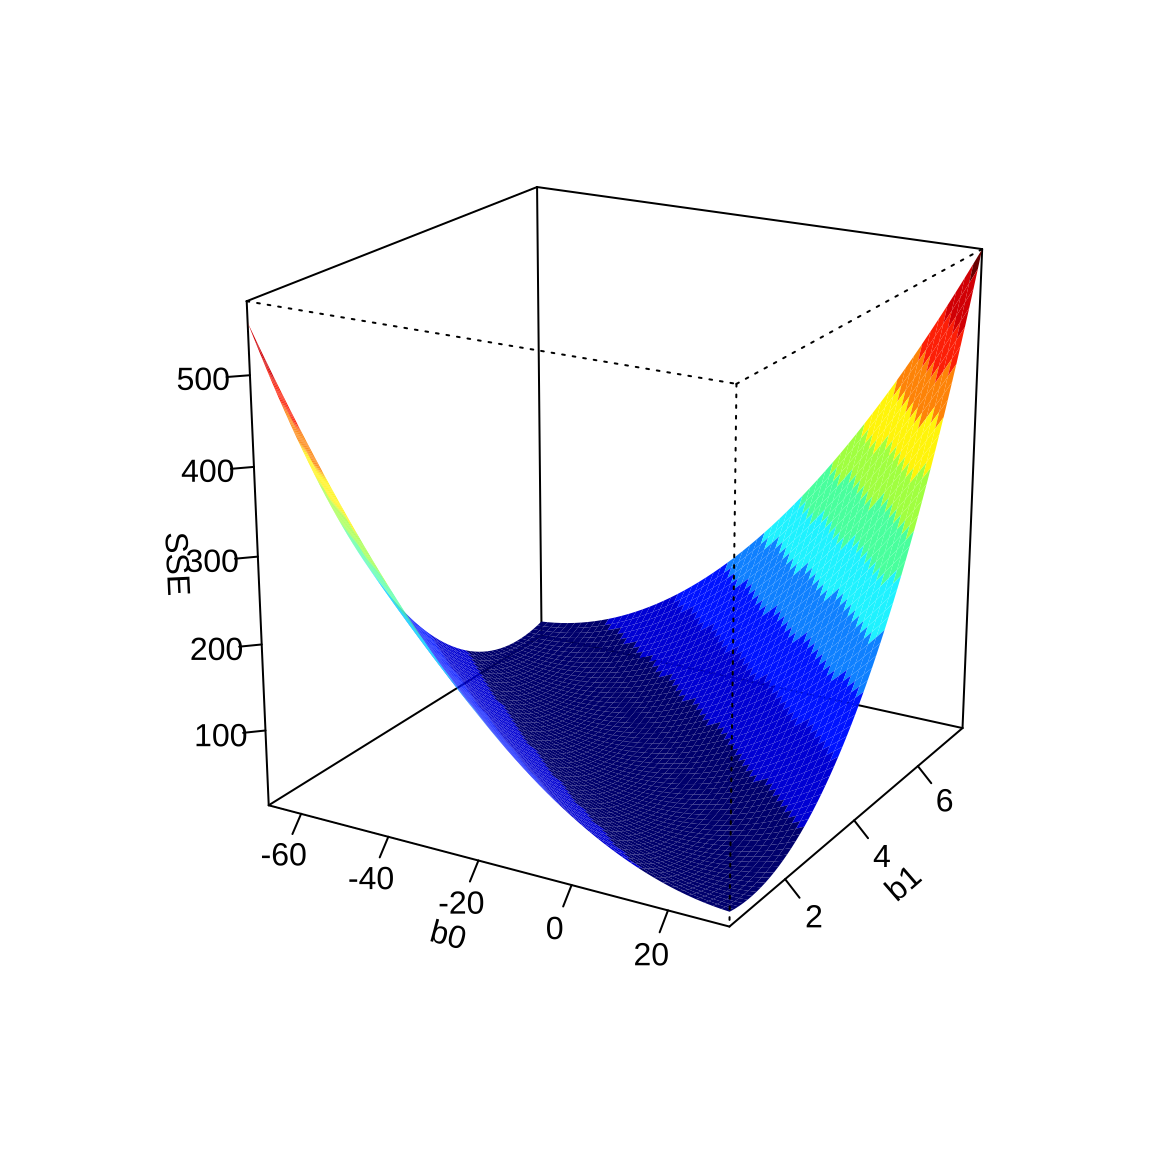
\includegraphics{lmbook_files/figure-latex/unnamed-chunk-8-1.pdf}

\begin{Shaded}
\begin{Highlighting}[]
\CommentTok{\# SSE의 그림을 쉽게 그리기 위하여 변수들을 표준화!}
\NormalTok{std\_cars }\OtherTok{\textless{}{-}} \FunctionTok{as.data.frame}\NormalTok{(}\FunctionTok{scale}\NormalTok{(cars))}
\NormalTok{gridnum }\OtherTok{\textless{}{-}} \DecValTok{60}
\NormalTok{sizing }\OtherTok{\textless{}{-}} \DecValTok{1}
\NormalTok{b0 }\OtherTok{\textless{}{-}} \FunctionTok{seq}\NormalTok{(}\DecValTok{0}\SpecialCharTok{{-}}\NormalTok{sizing,  }\DecValTok{0}\SpecialCharTok{+}\NormalTok{sizing, }\AttributeTok{length=}\NormalTok{gridnum )}
\NormalTok{b1 }\OtherTok{\textless{}{-}} \FunctionTok{seq}\NormalTok{(}\DecValTok{1}\SpecialCharTok{{-}}\NormalTok{sizing, }\DecValTok{1}\SpecialCharTok{+}\NormalTok{sizing, }\AttributeTok{length=}\NormalTok{gridnum )}

\NormalTok{SSE }\OtherTok{\textless{}{-}} \FunctionTok{matrix}\NormalTok{(}\DecValTok{0}\NormalTok{, gridnum, gridnum )}
\ControlFlowTok{for}\NormalTok{ (i }\ControlFlowTok{in} \DecValTok{1}\SpecialCharTok{:}\NormalTok{gridnum ) \{}
  \ControlFlowTok{for}\NormalTok{ (j }\ControlFlowTok{in} \DecValTok{1}\SpecialCharTok{:}\NormalTok{gridnum )\{}
\NormalTok{    r }\OtherTok{\textless{}{-}}\NormalTok{ std\_cars}\SpecialCharTok{$}\NormalTok{dist}\SpecialCharTok{{-}}\NormalTok{ b0[i] }\SpecialCharTok{{-}}\NormalTok{b1[j]}\SpecialCharTok{*}\NormalTok{std\_cars}\SpecialCharTok{$}\NormalTok{speed}
\NormalTok{    SSE[i,j]  }\OtherTok{\textless{}{-}} \FunctionTok{sum}\NormalTok{(r}\SpecialCharTok{\^{}}\DecValTok{2}\NormalTok{)}
\NormalTok{  \}}
\NormalTok{\}}
\FunctionTok{persp3D}\NormalTok{(b0, b1, SSE, }\AttributeTok{theta =}\DecValTok{40}\NormalTok{, }\AttributeTok{phi =} \DecValTok{15}\NormalTok{, }\AttributeTok{expand =} \DecValTok{1}\NormalTok{)}
\end{Highlighting}
\end{Shaded}

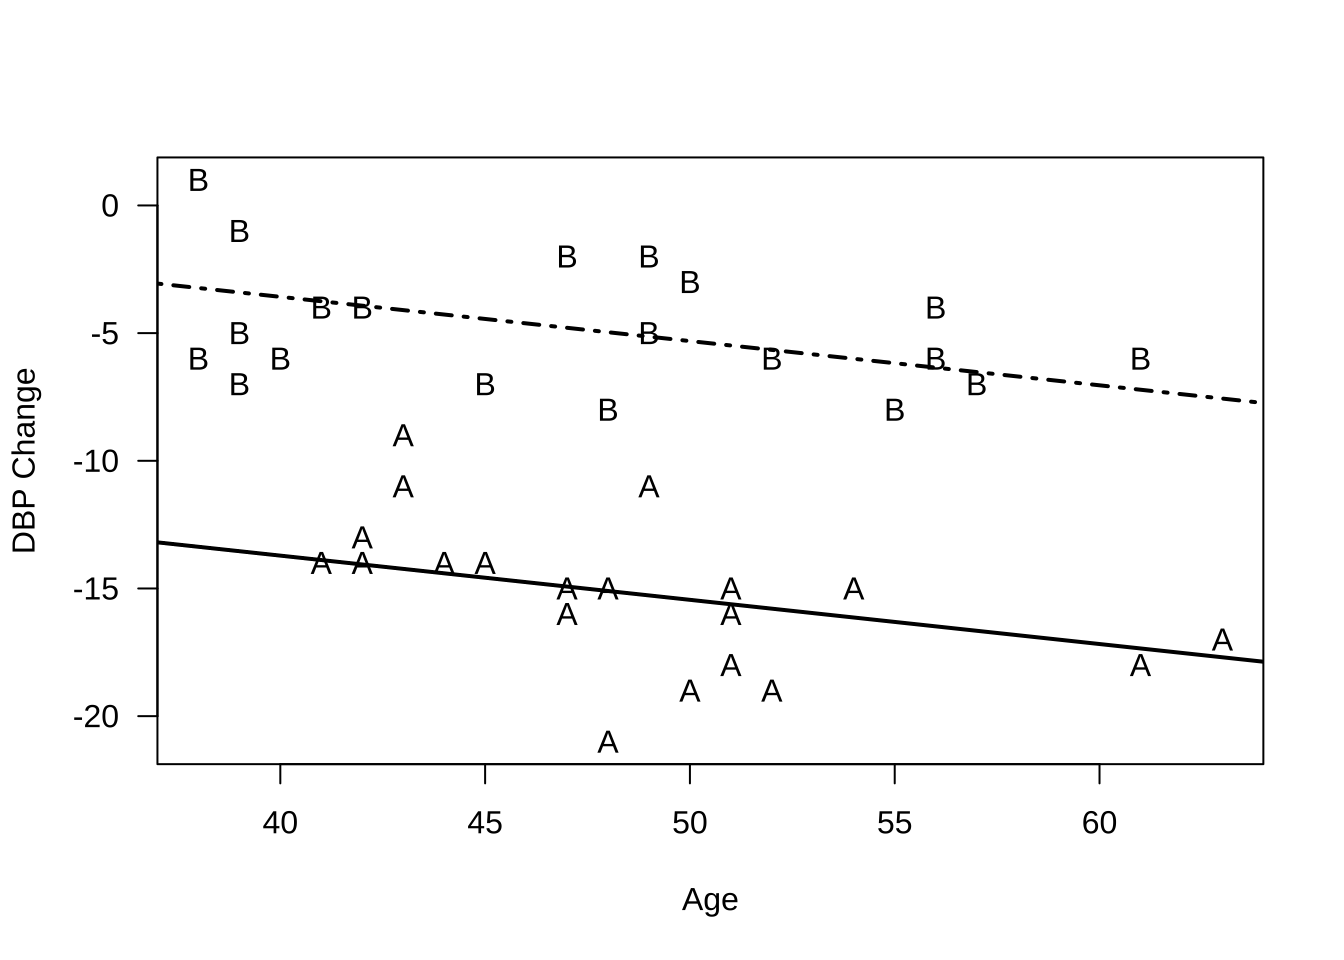
\includegraphics{lmbook_files/figure-latex/unnamed-chunk-9-1.pdf}

오차제곱합을 각 회귀계수에 대해서 편미분을 하고 0으로 놓으면 아래와 같이
두 방정식이 얻어진다.

\begin{align}
 \pardiff{ S(\beta_0 , \beta_1)}{\beta_0} & = \sum^n_{i=1}(-2)[y_i-(\beta_0+\beta_1 x_i)]=0  \label{eq:normaleq01}  \\ 
\pardiff{ S(\beta_0 , \beta_1)}{\beta_1}  & = \sum^n_{i=1}(-2 x_i)[y_i-(\beta_0+\beta_1 x_i)]=0 \label{eq:normaleq02}
\end{align} 위의 연립방정식을 행렬식으로 표시하면 다음과 같이 나타낼 수
있다.

\[ 
\begin{bmatrix}
n & \sum_i x_i \\
\sum_i x_i & \sum_i x^2_i
\end{bmatrix}
\begin{bmatrix}
\beta_0 \\
\beta_1
\end{bmatrix}
=
\begin{bmatrix}
\sum_i y_i \\
\sum_i x_i y_i
\end{bmatrix}
\]

위의 방정식을 풀어서 구한 회귀계수의 추정치를 \(\hat \beta_0\),
\(\hat \beta_1\) 이라고 하면 다음과 같이 주어진다.

\begin{align*}
 \hat \beta_0 &= \bar y - \hat \beta_1 \bar x  \\ 
  \hat \beta_1 &=  \frac{ \sum_i (x_i - \bar x)(y_i - \bar y)}{\sum_i (x_i - \bar x)^2} 
\end{align*}

최소제곱법에서 얻어진 회귀계수의 추정량 \(\hat \beta_0\)과 \(\hat \beta_1\)
을 이용한 반응변수 \(y_i\) 에 대한 예측값 \(\hat y_i\)는 다음과 같이
정의되고

\[ \hat y_i = \hat E(y_i|x_i) = \hat \beta_0 + \hat \beta_1 x_i \]

잔차 \(r_i\)는 다음과 같이 계산한다.

\begin{equation}
r_i = y_i - (\hat \beta_0 + \hat \beta_1 x_i) = y_i -\hat y_i  
\label{eq:residual}
\end{equation}

잔차 \(r_i\)는 다음과 같은 성질을 가진다.

\begin{enumerate}
\def\labelenumi{\arabic{enumi}.}
\tightlist
\item
  \(\sum_{i=1}^n r_i = 0\)
\item
  \(\sum_{i=1}^n x_i r_i = 0\)
\end{enumerate}

이제 위에서 본 \texttt{cars} 자료를 가지고 선형회귀모형 \eqref{eq:linreg02} 에
나타난 회귀계수를 추정해보자. 아래는 \texttt{R} 프로그램에서 함수 \texttt{lm}을 이용한
추정결과이다.

\begin{Shaded}
\begin{Highlighting}[]
\NormalTok{lmOut }\OtherTok{\textless{}{-}} \FunctionTok{lm}\NormalTok{(dist}\SpecialCharTok{\textasciitilde{}}\NormalTok{speed, }\AttributeTok{data=}\NormalTok{cars)}
\FunctionTok{summary}\NormalTok{(lmOut)}
\end{Highlighting}
\end{Shaded}

\begin{verbatim}
## 
## Call:
## lm(formula = dist ~ speed, data = cars)
## 
## Residuals:
##     Min      1Q  Median      3Q     Max 
## -29.069  -9.525  -2.272   9.215  43.201 
## 
## Coefficients:
##             Estimate Std. Error t value Pr(>|t|)    
## (Intercept) -17.5791     6.7584  -2.601   0.0123 *  
## speed         3.9324     0.4155   9.464 1.49e-12 ***
## ---
## Signif. codes:  0 '***' 0.001 '**' 0.01 '*' 0.05 '.' 0.1 ' ' 1
## 
## Residual standard error: 15.38 on 48 degrees of freedom
## Multiple R-squared:  0.6511, Adjusted R-squared:  0.6438 
## F-statistic: 89.57 on 1 and 48 DF,  p-value: 1.49e-12
\end{verbatim}

위에서 주어진 선형회귀모형 \eqref{eq:linreg02} 에 대한 추정 결과를
이용하면 자동차의 속도(\(x\) = \texttt{speed})와 제동거리(\(y\) = \texttt{dist})의 관계는
다음과 같은 회귀식으로 나타낼 수 있다.

\begin{Shaded}
\begin{Highlighting}[]
\NormalTok{equatiomatic}\SpecialCharTok{::}\FunctionTok{extract\_eq}\NormalTok{(lmOut, }\AttributeTok{use\_coefs =} \ConstantTok{TRUE}\NormalTok{)}
\end{Highlighting}
\end{Shaded}

\[
\operatorname{\widehat{dist}} = -17.58 + 3.93(\operatorname{speed})
\]

위의 추정식을 이용하면 주어진 자동차의 속도에서 제동거리를 예측할 수
있다. 예를 들어 자동차의 속도가 25 mph인 경우에는 제동거리의 평균이
80.73 mph 임을 알 수 있다.

\[ E(y|x=25) = −17.58 + 3.93 (25) = 80.73 \]

\begin{Shaded}
\begin{Highlighting}[]
\NormalTok{newcars }\OtherTok{\textless{}{-}} \FunctionTok{data.frame}\NormalTok{(}\AttributeTok{speed =} \FunctionTok{c}\NormalTok{(}\DecValTok{25}\NormalTok{))}
\FunctionTok{predict}\NormalTok{(lmOut, }\AttributeTok{newdata=}\NormalTok{newcars)}
\end{Highlighting}
\end{Shaded}

\begin{verbatim}
##        1 
## 80.73112
\end{verbatim}

기울기의 추정값 \(\hat \beta_1 = 3.93\) 은 자동차의 속도 (\(x\))가 1 mph
증가할 때 평균 제동거리 (\(E(y|x)\))가 3.93 ft 증가한다는 의미이다.

\[ \hat E(y | x) = −17.58 + 3.93 x \]

\hypertarget{rsquare}{%
\subsection{결정계수}\label{rsquare}}

고려한 독립변수와 반응변수에 대하여 제시된 회귀식을 적합한 후 회귀모형이 두 변수의 관계를 얼마나 잘 설명하는지에 대한 기준이 필요하다. 회귀식의 적합에 대한 기준으로서
결정계수(coefficient of determination; \(R^2\))가 있다. 결정계수는 적합의
정도(degree of fitting)를 측정한다. 즉 ``독립변수는 반응변수를 얼마나 잘
예측하느냐''에 대한 정도를 수치로 표현한 것이다.

회귀분석에서 독립변수와 반응변수 간에 전혀 회귀관계가 없다면 당연히
반응변수의 값은 독립변수 값의 변동 여하에 전혀 영향을 받지 않아야 한다.
단순회귀모형에서 독립변수 \(x\)의 값의 변화를 반응변수 \(y\)로 값으로
표현하는것이 바로 기울기 \(\beta_1\)이다. 이렇게 고려한 독립변수 \(x\)가 반응변수 \(y\)를 예측하는데 전혀 소용이 없다면 이는 기울기에 대한 회귀계수가 0 \(\beta_1=0\) 이라는 것을 의미이다.
이러한 경우에 대하여 다음과 같은 모형을 생각할 수 있다.

\begin{equation}
y_i = \beta_0 +e_i, \quad e_i \sim (0,\sigma^2) 
\label{eq:meanmodel}
\end{equation}

위와 같은 경우에 대한 모형을 \eqref{eq:meanmodel} 과 같이 표현할 수 있으며 평균 모형(mean model)이라고 부른다.
평균 모형은 우리가 생각할 수 있는 모형 중에서 가장 간단한, 하지만 별로 쓸모없는 모형이라고 할 수 있다.
이러한 평균 모형에 대한 최소제곱법을 적용하여 \(\beta_0\)의 추정량을
구하면 추정량 \(\hat \beta_0\)는 \(\bar y\)가 된다. 그 이유는 위의 모형에
오차제곱합을 구해보면 다음과 같은 형식이 된다

\[ S(\beta_0)=  \sum^n_{i=1}[y_i-\beta_0]^2 \]

여기서 \(\beta_0\)에 대하여 최고로 하는 지점을 찾아보면 다음과 같은 방정식을 얻을 수 있다.

\[ \frac{\partial S(\beta_0)}{\partial \beta_0}  = 0  \Rightarrow  \sum^n_{i=1}[y_i - \beta_0] = 0 \]
이 방정식을 풀면 \(\hat \beta_0 = \bar y\)가 됨을 알 수 있다. 결국
독립변수가 반응변수에 아무른 영향을 주지 못하게 되면 \(y\)의 예측값은 평균
\(\bar y\)임을 알 수 있다 (평균모형 \eqref{eq:meanmodel} 경우 \(\bar y\)는
\(\beta_0\) 의 최소제곱추정량이다).

여기서 주목해야할 점은 평균 모형 \eqref{eq:meanmodel} 에서의 잔차 \(r_{0i}\)는 다음과 같이 정의된다.

\[ r_{0i} = y_i -\hat \beta_0 = y_i - \bar y \]

주어진 회귀식이 유의한 경우, 즉 회귀식의 기울기가 0이 아닌 경우 (\(\beta_1 \ne 0\)) 적합된 회귀식에 대한 잔차는 식 \eqref{eq:residual} 과 같이 나타난다. 만약 회귀식이 유의하다면 식 \eqref{eq:residual} 으로 구해진 잔차 \(r_i = y_i -\hat \beta_0 - \hat \beta_1 x_i\) 와 평균 모형에서 구해지는 잔차 \(r_{0i} = y_i - \bar y\) 간의 어떤 차이가 있을까? 아래의 그림은 앞의 예제 자료에 대하여 설명변수가 없는 평균 모형(파란 선)과 설명변수가 있는 회귀모형(빨간 선)을 나타낸 그림이다. 잔차는 적합된 직선과 반응 변수 간의 차이를 의미하며 차이의 절대값이 작을 수록 좋은 모형이다.

\begin{Shaded}
\begin{Highlighting}[]
\FunctionTok{ggplot}\NormalTok{(cars, }\FunctionTok{aes}\NormalTok{(}\AttributeTok{x=}\NormalTok{speed, }\AttributeTok{y=}\NormalTok{dist)) }\SpecialCharTok{+}
     \FunctionTok{geom\_point}\NormalTok{() }\SpecialCharTok{+}
     \FunctionTok{labs}\NormalTok{(}\AttributeTok{x =} \StringTok{"속도"}\NormalTok{, }\AttributeTok{y =} \StringTok{"거리"}\NormalTok{) }\SpecialCharTok{+}
     \FunctionTok{geom\_smooth}\NormalTok{(}\AttributeTok{method =}\NormalTok{ lm, }\AttributeTok{color=}\StringTok{\textquotesingle{}red\textquotesingle{}}\NormalTok{, }\AttributeTok{se =} \ConstantTok{FALSE}\NormalTok{) }\SpecialCharTok{+}
     \FunctionTok{geom\_hline}\NormalTok{(}\AttributeTok{yintercept =} \FunctionTok{mean}\NormalTok{(cars}\SpecialCharTok{$}\NormalTok{dist), }\AttributeTok{color=}\StringTok{\textquotesingle{}blue\textquotesingle{}}\NormalTok{)}
\end{Highlighting}
\end{Shaded}

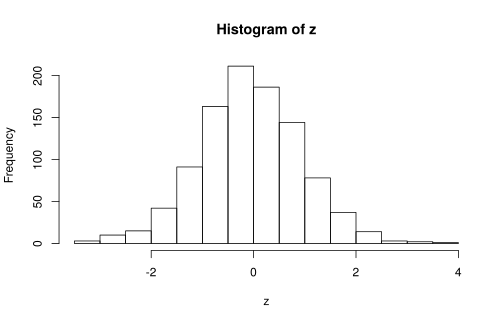
\includegraphics{lmbook_files/figure-latex/unnamed-chunk-13-1.pdf}

잔차의 절대값보다 제곱한 양이 다루기가 쉬우므로(why?) 평균 모형과 회귀 모형의 적합도를 비교하는 양으로서 다음과 같은 각각의 모형에서 나온 두개의 잔차제곱합을 생각할 수 있다.

먼저 평균 모형은 예측에 사용할 변수가 없는 경우로서 이때의 잔차는 각 관측값에 대한 예측값이 관측값의 평균이다 . 이러한 경우 잔차는 관측값 자체가 가지고 있는 변동으로 생각할 수 있다. 이러한 평균모형에서의 잔차 또는 관측값이 가지고 있는 변동을 총제곱합(Total Sum of Squares ; \(SST\))이다

\begin{align*}
\sum_{i=1}^n r^2_{0i} & = \sum_{i=1}^n (y_i -\bar y)^2 \\
  & =  \text{ Residual Sum of Squares from mean model }  \\
   & = \text{ Variation of response variables} \\
   & = \text{ Total Sum of Squares } \\
   & = SST
\end{align*}

이제 독립변수가 있는 회귀모형에서 예측치 \(\hat y_i=\hat \beta_0 + \hat \beta_1 x_i\)를 고려하면
이 경우의 잔차들의 제곱합은 회귀식의 잔차제곱합(Residual Sum of Squares; \(SSE\))이라고 부르며 아래와 같이 정의한다.

\begin{align*}
\sum_{i=1}^n r_i^2 & = \sum_{i=1}^n (y_i -\hat \beta_0 - \hat \beta_1 x_i) \\
  & = \text{Residual Sum of Squares from linear regression model } \\
  & = \text{ Residual Sum of Squares } \\
  & = SSE 
\end{align*}

만약 회귀식에서 고려한 설명변수가 반응변수를 예측하는데 매우 적합하다면 회귀모형에서 구한 잔차들의 제곱합이 평균모형에서 구한 잔차들의 제곱합보다 작을 것이다. 이러한 차이를 비교하려면 두 제곱합 \(SST\) 와 \(SSE\)의 관계를 이해하는 것이 중요하다.

두 제곱합 \(SST\) 와 \(SSE\)의 관계를 보기 위하여 먼저 두 잔차 \(r^0_i\) 와 \(r_i\)의 차이를 비교해 보자

\[ r^0_i - r_i = (y_i - \bar y) - (y_i - \hat y_i) = \hat y_i - \bar y \]

위의 식에서 두 잔차의 차이 \(\hat y_i - \bar y\)는 예측값과
평균 간 차이로서 그 절댸값이 크면 회귀직선이 반응변수를 설명할 수 있는 능력이 크다는 것을 의미한다.

위의 식을 다시 쓰면 다음과 같다.

\[  (y_i - \bar y) = (y_i - \hat y_i) + (\hat y_i - \bar y) \]

즉, (평균모형의 잔차)=(회귀모형의 잔차))+(회귀모형의 설명부분)으로 분해되는 것으로 이해할 수 있다. 이 분해에서 회귀모형의 잔차가 작을수록 회귀 모형의 예측 능력, 즉 적합도가 커지는 것을 알 수 있다.

이제 총제곱합은 다음과 같이 분해할 수 있다.

\begin{eqnarray*}
 \sum^n_{i=1}(y_i - \bar y)^2 &= & \sum^n_{i=1}[(y_i-\hat y_i)+(\hat y_i - \bar y)]^2 \\
 &=& \sum^n_{i=1}(y_i-\hat y_i)^2+\sum^n_{i=1}(\hat y_i - \bar y)^2
        + 2\sum^n_{i=1}(y_i-\hat y_i)(\hat y_i-\bar y)  \\
 &=& \sum^n_{i=1}(y_i-\hat y_i)^2+\sum^n_{i=1}(\hat y_i - \bar y)^2 + 0 \quad \text{(why?)}
 \end{eqnarray*}

따라서 다음과 같은 제곱합의 분해를 얻게 된다.

\[ \sum^n_{i=1}(y_i - \bar y)^2 = \sum^n_{i=1}(y_i-\hat y_i)^2+\sum^n_{i=1}(\hat y_i - \bar y)^2\]
여기서 모형제곱합(regression sum of
square; SSR)를 다음과 같이 정의하면
\[  SSR = \sum^n_{i=1}(\hat y_i-\bar y_i)^2 \]

총제곱합은 잔차제곱합 과 모형제곱합으로 분해된다.

\begin{equation}
 SST = SSE + SSR 
\label{eq:ssqdecomp}
\end{equation}

관측값들이 보여주는 총 변동인 총제곱합(SST)에서 회귀모형으로 설명할 수
있는 변동, 즉 모형제곱합(SSR)이 차지하는 비율을 결정계수(coefficient of
determination)라 하며 \(R^2\)으로 표현한다.

\[ R^2 = \frac{SSR}{SST} =  1 -\frac{SSE}{SST}  =1- \frac{\sum^n_{i=1}(y_i-\hat y_i)^2}{ \sum^n_{i=1}(y_i - \bar y)^2} \]
위에서 정의된 \(R^2\) 는 평균 모형의 잔차제곱합 \(SST\)과 회귀모형의 잔차제곱합 \(SSE\)의 비율로 정의되는 것으로 해석할 수 있다.
즉,

\[  R^2 = 1 -\frac{SSE}{SST} =1 -\frac{\text{Residual SS from regression model}}{\text{Residual SS from mean model}} \]

결정계수의 정의를 보면 회귀모형의 잔차제곱합(\(SSE\))가 평균 모형의 잔차제곱합(\(SST\))에 대하여 \textbf{상대적으로} 작아질수록 결정계수가 커진다. 결정계수 \(R^2\)는 언제나 0 이상 1 이하의 값을 갖는다. 회귀모형이
데이터에 아주 잘 적합되면 결정계수의 값은 1 에 가깝게 된다.

\hypertarget{uxc911uxd68cuxadc0-uxbaa8uxd615}{%
\section{중회귀 모형}\label{uxc911uxd68cuxadc0-uxbaa8uxd615}}

일반적으로 회귀모형에서 반응변수의 수는 하나인 경우가 많지만 설명변수의
수는 여러 개인 경우가 많다. 이런 경우 중선형 회귀 모형(multiple linear
regression)은 다음과 같이 표현할 수 있고, \(p-1\)개의 설명변수가 있다고
가정하고 \((x_1, x_2, \cdots, x_{p-1})\) 표본의 크기 \(n\)인 자료가 얻어지면
선형회귀식을 행렬로 다음과 같이 표현할 수 있다.

\begin{equation*}
y_i = \beta_0 + \beta_1 x_{i1} + \beta_2 x_{i2} + \cdots + \beta_{p-1} x_{i,p-1} +  e_i = \bm x^t_i \bm \beta +  e_i 
\end{equation*}

\begin{rmdimportant}
독립변수의 개수를 \(p\)개로 하면 절편을 포함해서 계획행렬 \(\bm X\)의 차원이 \(n \times (p+1)\)이 된다. 이렇게 차원을 \(p+1\)로 사용하면 불편하므로 독립변수의 수를 \(p-1\) 로 하여 계획행렬의 차원을 \(n \times p\) 놓는다. 다른 교과서에서는 독립변수의 수를 \(p\) 개로 모형을 정의하기도 한다.
\end{rmdimportant}

위의 식을 다시 표현하면 다음과 같이 쓸 수 있다.

\[ 
y_i  = \bm x^t_i \bm \beta  + e_i  =
\begin{bmatrix}
1 & x_{i1} & x_{i2} & \cdots & x_{i,p-1}
\end{bmatrix}
\begin{bmatrix}
\beta_{0} \\
\beta_{1} \\
\beta_{2} \\
\vdots \\
\beta_{p-1}
\end{bmatrix}
+ e_i
\]

이제 \(n\)개의 관측치 \(y_1,y_2, \dots, y_n\) 으로 이루어진 관측값 벡터
\(\bm y\)를 고려하면 n개의 관측치에 대한 회귀식을 행렬식으로 다음과 같이
표현할 수 있다.

\[ 
\begin{bmatrix}
y_{1} \\
y_{2} \\
\vdots \\
y_{n}
\end{bmatrix} =
\begin{bmatrix}
1 & x_{11} & \cdots & x_{1,p-1} \\
1 & x_{21} & \cdots & x_{2,p-1} \\
\vdots & \vdots & \vdots & \vdots \\
1 & x_{n1} & \cdots & x_{n,p-1}
\end{bmatrix}
\begin{bmatrix}
\beta_{0} \\
\beta_{1} \\
\vdots \\
\beta_{p-1}
\end{bmatrix}
+
\begin{bmatrix}
 e_{1} \\
 e_{2} \\
\vdots \\
 e_{n}
\end{bmatrix}
\]

위의 식을 간단히 행렬식으로 표시하면 다음과 같다.

\begin{equation} 
\bm y = \bm X \bm \beta + \bm e
\label{eq:multireg2}
\end{equation}

위의 행렬식에서 각 벡터와 행렬의 차원은 다음과 같다.

\begin{itemize}
\tightlist
\item
  \(\bm y\): \(n \times 1\)
\item
  \(\bm X\): \(n \times p\)
\item
  \(\bm \beta\): \(p\times 1\)
\item
  \(\bm e\): \(n \times 1\)
\end{itemize}

여기서 회귀분석의 오차항 \(e_i\)은 서로 독립이고 동일한 분산을 갖는다. 즉,
오차항은 다음의 분포를 따른다.
\[ \bm e  \sim (\bm 0,\sigma^2 \bm I_n) \]

따라서 관측값 벡터 \(\bm y\)의 평균은 다음과 같고

\begin{equation}
 E(\bm y|\bm X) = E(\bm X \bm \beta+\bm e)= \bm X \bm \beta + E(\bm e) = \bm X \bm \beta
\label{eq:multiregmean}
\end{equation}

\(\bm y\)의 분산은 아래와 같이 주어진다.

\begin{equation}
 V( \bm y| \bm X) = E[( \bm y -  \bm X \bm \beta)( \bm y -  \bm X \bm \beta)^t] = E( \bm  e   \bm  e^t) = \sigma^2 \bm I_n
\label{eq:multiregvar}
\end{equation}

여기서 오차항이 정규분포를 따른다면

\[ \bm  e   \sim N(\bm 0,\sigma^2 \bm I_n) \]

관측값 벡터 \(\bm y\) 또한 정규분포를 따른다

\[  \bm y \sim N( \bm X \bm \beta, \sigma^2 \bm I_n) \]

\hypertarget{uxcd5cuxc18cuxc81cuxacf1uxcd94uxc815}{%
\subsection{최소제곱추정}\label{uxcd5cuxc18cuxc81cuxacf1uxcd94uxc815}}

최소제곱추정법(least square estimation)은 자료의 관계을 잘 반영하는
회귀식을 구한 다음 실제 관측값 \(y_i\)과 예측값 \(\bm x_i^t \bm \beta\) 간에
차이인 잔차를 가장 작게 만드는 것이 목적이다. 모든 잔차항의 제곱의 합을
최소화하는 방법을 최소제곱법이라고 하며 이를 이용하여 회귀계수의
추정량을 찾는다.

\begin{equation} 
 \min_{\bm \beta} \sum_{i=1}^n (y_i -  \bm x_i^t \bm \beta )^2 = \min_{\bm \beta } ( \bm y -  \bm X \bm \beta )^t( \bm y -  \bm X \bm \beta ) 
 \label{eq:rsq2}
 \end{equation}

\hypertarget{uxbc29uxbc95-1}{%
\subsection{방법 1}\label{uxbc29uxbc95-1}}

\(\hat {\bm \beta}\)는 잔차의 제곱합 \eqref{eq:rsq2} 을 최소로 하는
최소제곱 추정량이다. 잔차의 제곱합을 \(S( \bm \beta)\)이라고 하면

\begin{align} 
S( \bm \beta ) & =  ( \bm y -  \bm X \bm \beta)^t( \bm y -  \bm X \bm \beta ) \notag \\
  & = \bm y^t \bm y - \bm y^t \bm X \bm \beta - \bm \beta^t \bm X^t \bm y
    + \bm \beta^t \bm X^t \bm X \bm \beta \notag \\
  & = \bm y^t \bm y -2  \bm \beta^t \bm X^t \bm y
    + \bm \beta^t \bm X^t \bm X \bm \beta \label{eq:rsq3}   
\end{align}

여기서 \(S( \bm \beta)\)를 최소로 하는 회귀계수벡터의 값을 구하기 위하여
\(S( \bm \beta)\)를 회귀계수벡터 \(\bm \beta\)로 미분한후 \(\bm 0\) 으로 놓고
선형 방정식을 풀어야 한다.

앞 절에 나오는 벡터미분을 이용하면

\begin{align*}
 \pardiff{ S( {\bm \beta})}{\bm \beta} & = 
 \pardiff{}{\bm \beta} (\bm y^t \bm y -2  \bm \beta^t \bm X^t \bm y
    + \bm \beta^t \bm X^t \bm X \bm \beta) \\
 & = \bm 0 -2 \bm X^t \bm y + 2 \bm X^t \bm X \bm \beta \\
 & =\bm 0
 \end{align*}

최소제곱 추정량을 구하기 위한 정규방정식은 다음과 같이 쓸 수 있다.

\begin{equation} 
 \bm X^t \bm X \bm \beta =  \bm X^t \bm y
 \label{eq:lsequation}
\end{equation}

방정식 \eqref{eq:lsequation}를 정규방정식(normal equation)이라고 한다.
만약 \(\bm X^t \bm X\)가 정칙행렬일 경우 최소제곱법에 의한 회귀계수 추정량
\(\hat {\bm \beta}\) 다음과 같다.

\begin{equation}
  \hat {\bm \beta} = ( \bm X^t \bm X)^{-1} \bm X^t \bm y
  \label{eq:lsestimator}
\end{equation}

예측값 벡터 \(\hat {\bm y}\) 는 \(E(\bm y | \bm X)\)의 추정치로서 다음과
같다.

\[ \hat E(\bm y | \bm X)= \hat {\bm y} = \bm X \hat {\bm \beta} = \bm  X(\bm X^t \bm X)^{-1} \bm X^t y \]

만약 \(\bm X^t \bm X\)가 정칙행렬이 아닐 경우 최소제곱법에 의한 회귀계수
추정량 \(\hat {\bm \beta}\)은 \(\bm X^t \bm X\)의 일반화 역행렬
\((\bm X^t \bm X)^-\)를 이용하여 다음과 같이 구한다. 이 경우 일반화
역행렬이 유일하지 않기 때문에 회귀계수 추정량도 유일하지 않다.

\[
  \hat {\bm \beta} = ( \bm X^t \bm X)^{-} \bm X^t \bm y
\]

\hypertarget{uxbc29uxbc95-2}{%
\subsection{방법 2}\label{uxbc29uxbc95-2}}

식 \eqref{eq:rsq2}에서 나오는 오차벡터를 정의하고
\(\bm e = (\bm y - \bm X \bm \beta)\) 오차벡터를 모수벡터 \(\bm \beta\)로
미분하면 다음과 같은 결과를 얻는다.

\[ \pardiff{\bm e}{\bm \beta} = \pardiff{ (\bm y - \bm X \bm \beta)}{ \bm \beta} =
- \pardiff{ \bm X \bm \beta}{ \bm \beta} \equiv
- \pardiff{\bm \beta^t \bm X^t }{\bm \beta} = -\bm X^t \]

이제 오차제곱합 \(S( {\bm \beta})=\bm e^t \bm e\) 를 모수벡터로 미분하면
이차형식의 미분공식과 합성함수 미분공식을 차례로 적용하면 된다.
\[  \pardiff{ S( {\bm \beta})}{\bm \beta}=\pardiff{\bm e^t \bm e}{\bm \beta} =  \pardiff{\bm e }{\bm \beta} \pardiff{\bm e^t  \bm e}{\bm e} = -\bm X^t \left( 2 \bm e \right ) = -2 \bm X^t (\bm y - \bm X \bm \beta)  \]

위의 방정식을 \(\bm 0\)으로 놓으면 최소제곱 추정량 (열)벡터를 구한다.
\[ \bm X^t \bm y - \bm X^t  \bm X \bm \beta = \bm 0 \quad \rightarrow \quad
\hat{\bm \beta}  = (\bm X^t  \bm X)^{-1} \bm X^t  \bm y \]

\hypertarget{uxcd5cuxc18cuxc81cuxacf1-uxcd94uxc815uxb7c9uxc758-uxbd84uxd3ec}{%
\section{최소제곱 추정량의 분포}\label{uxcd5cuxc18cuxc81cuxacf1-uxcd94uxc815uxb7c9uxc758-uxbd84uxd3ec}}

회귀선을 추정하기 위한 회귀계수 추정값인 \(\hat {\bm \beta}\)의 분포를 알아보기
위해서 우선 선형추정량을 보면 다음과 같다.

\[ \hat {\bm \beta}  = (\bm X^t\bm X)^{-1}\bm X' \bm y \equiv  \bm M \bm y \]
따라서 최소제곱 추정량은 관측값들의 선형 변환이다. 회귀계수 추정값
\(\hat {\bm \beta}\)의 기대값은 \begin{eqnarray*}
 E( \hat {\bm \beta}  ) &=& E( \bm M \bm y) = E(( \bm X^t \bm X)^{-1} \bm X' \bm y) \\
 &=& ( \bm X^t \bm X)^{-1} \bm X'E( \bm y) \\
 &=& ( \bm X^t \bm X)^{-1} \bm X^t \bm X \bm \beta \\
  &=& \bm \beta
\end{eqnarray*}

따라서 최소제곱 추정량 \(\hat {\bm \beta}\)는 \(\bm \beta\)의 불편추정량이다. 최소제곱
추정량 \(\hat {\bm \beta}\)의 공분산 행렬을 전개해보면 \begin{eqnarray*}
 Var( \hat {\bm \beta} ) &=& Var(( \bm X^t \bm X)^{-1} \bm X^t \bm y) \\
&=& ( \bm X^t \bm X)^{-1} \bm X^t ~ Var( \bm y) ~ \bm X ( \bm X^t \bm X)^{-1} \\
&=&( \bm X^t \bm X)^{-1} \bm X^t[\sigma^2  \bm I_n] \bm X( \bm X^t \bm X)^{-1} \\
&=& \sigma^2( \bm X^t \bm X)^{-1} \bm X^t \bm X( \bm X^t \bm X)^{-1} \\
&=& \sigma^2( \bm X^t \bm X)^{-1} \\
\end{eqnarray*}

위에서 최소제곱 추정량의 평균과 공분산을 구할 때에는 정규성 가정이
필요하지않다. 만일 \(\bm y\)가 정규분포를 따른다면 \(\bm y\)의
선형변환으로부터 얻어진 \(\hat {\bm \beta}\)의 분포는 정규분포이며 다음과 같다.

\[  \hat {\bm \beta}  \sim N \left (\bm \beta, \sigma^2( \bm X^t \bm X)^{-1} \right ) \]

\hypertarget{uxac00uxc6b0uxc2a4-uxc815uxb9ac}{%
\section{가우스 정리}\label{uxac00uxc6b0uxc2a4-uxc815uxb9ac}}

\begin{theorem}
\protect\hypertarget{thm:unnamed-chunk-15}{}{\label{thm:unnamed-chunk-15} }선형회귀모형 \(\bm y = \bm X \bm \beta + \bm e\)에서 \(E( \bm e)=0, Var( \bm e)=\sigma^2 \bm I\)이 성립하면 최소제곱 추정량

\[ \hat{\bm \beta}=(\bm X^t \bm X)^{-1} \bm X^t \bm y\]

는 \(\bm \beta\)의 최소분산 선형 불편추정량이다.
\end{theorem}

위의 정리를 Gauss-Markov 정리라고 하며 이는 회귀계수 \(\bm \beta\)의 모든
선형 불편 추정량들 중에 최소제곱 추정량
\(\hat {\bm \beta}=(\bm X^t \bm X)^{-1} \bm X^t \bm y\)이 가장 작은 분산을
가짐을 뜻한다 (Best Linear Unbiased Estimator; BLUE).

Gauss-Markov 정리를 정확하게 표현하면 \(E(\bm L \bm y) = \bm \beta\)를
만족하는 모든 \(n \times n\) 차원의 행렬 \(\bm L\)과 임의의 벡터 \(\bm c\)에
대하여 다음이 성립한다.

\[ V(\bm c^t \hat {\bm \beta}) \le V(\bm c^t \bm L \bm y)  \]

Gauss-Markov 정리를 증명해보자. 관측벡터 \(\bm y\)에 대한 임의의 선형
추정량 \(\bm \beta^* = \bm L \bm y\)를 생각해보면 다시 다음의 형태로
표시할 수 있다.
\[  \bm \beta^* =  \bm L  \bm y = (\bm M + \bm L -\bm M ) \bm y = ( \bm M +  \bm A)  \bm y \]
여기서 \(\bm M = ( \bm X^t \bm X)^{-1} \bm X^t\) 이고
\(\bm A= \bm L- \bm M\) 이다. 임의의 선형 추정량 \(\bm \beta^*\)가 불편
추정량일 조건을 구해보자 \begin{align*}
 E( \bm \beta^*) & = E[( \bm M+ \bm A) \bm y] \\
            & = ( \bm M+ \bm A)E( \bm y) \\
            & = ( \bm M+ \bm A)X \bm \beta \\
            & = ( \bm X^t  \bm X)^{-1} \bm X^t  \bm X  \bm \beta +  \bm A  \bm X  \bm \beta \\
            & =  \bm \beta+AX \bm \beta\\
\end{align*} 여기서 불편추정량이 되기 위해서는
\(E( \bm \beta^*)= \bm \beta\) 조건을 만족 해야되며 따라서
\(\bm A \bm X=0\)이되어야한다 (이 조건은 \(\bm A=0\)를 의미하는 것은
아니다).

이제 최소분산을 가지기 위해서 \(\bm A \bm X=0\)을 만족하는 행렬
\(\bm A\)중에서 \(Var( \bm \beta^*)\)을 최소로하는 행렬 \(\bm A\)를 구해야
한다. \(\bm \beta^*\)의 공분산 행렬은 \(AX=0\)이므로 \begin{align*}
 V( \bm \beta^*) & = ( \bm M+ \bm A)V( \bm y)( \bm M+ \bm A)^t\\
            & = ( \bm M+ \bm A)\sigma^2 I_n( \bm M+ \bm A)^t\\
            & = \sigma^2 ( \bm M \bm M^t+ \bm A \bm M^t+ \bm M  \bm A^t+ \bm A  \bm A^t)\\
            & = \sigma^2 [ ( \bm X^t  \bm X)^{-1}  \bm X^t  \bm X( \bm X^t \bm X)^{-1} + \bm A  \bm X ( \bm X^t  \bm X)^{-1}+( \bm X^t  \bm X)^{-1} \bm X^t  \bm A^t+  \bm A  \bm A^t ]\\
            & = \sigma^2[( \bm X^t  \bm X)^{-1} +  \bm A  \bm A^t ]  \\
            & = V( \hat {\bm \beta} ) + \sigma^2 \bm A \bm A^t\\
\end{align*}

이제 임의의 벡터 \(\bm c\)에 대하여

\begin{align*}
 V( \bm c^t \bm \beta^*)  & = \bm c^t V (\bm \beta^*) \bm c \\
   & =  \bm c^t V( \hat {\bm \beta} ) \bm c + \sigma^2 \bm c^t \bm A \bm A^t \bm c \\
    & =  V( \bm c^t  \hat {\bm \beta} ) + \sigma^2 \bm c^t \bm A \bm A^t \bm c 
\end{align*}

다음이 성립하므로

\[ \bm c^t \bm A \bm A^t \bm c = \bm u^t \bm u = \sum_{i=1}^n u_i^2 \ge 0 \]

임의의 벡터 \(\bm c\)에 대하여

\[ V( \bm c^t \bm \beta^*) \ge  V( \bm c^t  \hat {\bm \beta} ) \]

이제 \(V( \bm c^t \bm \beta^*)\) 이 \(V( \bm c^t \hat {\bm \beta} )\)과
같으려면 다음 조건이 성립해야 하며

\[ \bm u = \bm c^t \bm A = \bm 0 \]

임의의 모든 벡터 \(\bm c\)에 대해서 위의 조건 성립해야 하므로 이는
\(\bm A = \bm 0\) 이 성립해야 한다. 또한 이조건은 \(\bm A \bm X=0\)도 만족
시켜준다. 따라서 \(\bm \beta\)의 최소분산 선형 불편추정량은 최소제곱법으로
구한 추정량이다.

여기서 주의할 점은 Gauss-Markov정리에서 관측값 \(\bm y\)에 대한 가정은
평균과 공분산의 가정만 주어졌으며 \(\bm y\)의 분포에 대한 가정이 없다.
참고로 만약에 \(\bm y\)가 정규분포를 따른다면 최소제곱 추정량은 최소분산
불편추정량이다.

\hypertarget{uxcd5cuxb300uxac00uxb2a5uxb3c4-uxcd94uxc815uxbc95}{%
\section{최대가능도 추정법}\label{uxcd5cuxb300uxac00uxb2a5uxb3c4-uxcd94uxc815uxbc95}}

관측값 벡터 \(\bm y\) 가 다음과 같이 선형모형이며 정규분포를 따른다고
가정하자.

\begin{equation}
\bm y \sim N( \bm X \bm \beta, \sigma^2 \bm I_n) 
\label{eq:normallm}
\end{equation}

선형모형 \eqref{eq:normallm}에 대한 가능도 함수는 다음과 같이 주어진다.

\begin{align*}
 L_n( \bm \theta ;  \bm y) & = L( \bm \beta,\sigma^2|  \bm y) \\
   & = \prod^n_{i=1} f(y_i)\\
   & = \prod^n_{i=1}(2 \pi \sigma^2)^{-\frac{1}{2}} \exp \left [-\frac{1}{2\sigma^2} (y_i- {\bm x}_i^t \bm \beta)^2 \right ] \\
   & = (2\pi\sigma^2)^{-\frac{n}{2}} \exp \left [ -\frac{1}{2\sigma^2}( \bm y- \bm  X  \bm \beta)^t( \bm y- \bm X  \bm \beta) \right ]
\end{align*}

또한 분산에 대한 모수를 \(\tau=\sigma^2\) 과 같이 쓰면 로그 가능도함수는
다음과 같다.

\begin{align*}
\ell_n( \bm \theta; \bm y) & = -\frac{n}{2} \log (2 \pi)-\frac{n}{2} \log \sigma^2 -\frac { ( \bm y- \bm X  \bm \beta)^t (\bm  y- \bm X  \bm \beta) }{2\sigma^2} \\ 
   &= -\frac{n}{2} \log (2 \pi)-\frac{n}{2} \log \tau -\frac { ( \bm y- \bm X  \bm \beta)^t ( \bm y- \bm X  \bm \beta) }{2\tau}  
\end{align*}

이제 로그가능도함수로부터 구할 수 있는 스코어함수 \(s( \bm \theta;\bm y)\) 와 그에
대한 관측 피셔정보 \(J_n( \bm \theta; \bm y)\) 은 다음과 같이 주어진다.

\begin{align*}
s( \bm \theta;  \bm y) & =  \pardiff{}{ \bm \theta}\ell_n( \bm \theta;  \bm y ) \\
  & =  \begin{bmatrix}
    \pardiff{}{ \bm  \beta}\ell_n( \bm \theta;  \bm y ) \\
    \pardiff{}{\tau}\ell_n( \bm \theta;  \bm y ) 
  \end{bmatrix} \\
  & = 
  \begin{bmatrix}
     \bm X^t ( \bm y- \bm X  \bm \beta)/\tau \\
    -\frac{n}{2\tau} +\frac { ( \bm y- \bm X  \bm \beta)^t ( \bm y- \bm X  \bm \beta) }{2\tau^2} 
  \end{bmatrix} \\
 J_n( \bm \theta;  \bm y) & =  -\pardiffdd{}{ \bm \theta}{ {\bm \theta}^t}\ell_n( \bm \theta;\bm y ) \\
  & = 
  - \begin{bmatrix}
    \pardiffdd{}{\bm \beta}{ {\bm \beta}^t}\ell_n( \bm \theta;\bm y ) & \pardiffdd{}{ \bm \beta}{\tau^t}\ell_n( \bm \theta;\bm y )  \\
    \pardiffdd{}{\tau}{ {\bm \beta}^t}\ell_n( \bm \theta;\bm y )  & \pardiffdd{}{\tau}{\tau}\ell_n( \bm \theta; \bm y ) 
  \end{bmatrix} \\
   & = 
  \begin{bmatrix}
      {\bm X}^t  \bm X /\tau &  - {\bm X}^t ( \bm y- \bm X  \bm \beta)/\tau^2   \\
    - {\bm X}^t ( \bm y- \bm X  \bm \beta)/\tau^2  &  - \frac{n}{2\tau^2} +\frac { ( \bm y- \bm X \bm  \beta)^t ( \bm y- \bm X  \bm \beta) }{\tau^3} 
  \end{bmatrix}
\end{align*}

\hypertarget{uxc120uxd615uxd68cuxadc0uxbaa8uxd615uxc5d0uxc11cuxc758-uxcd5cuxb300uxac00uxb2a5uxb3c4-uxcd94uxc815uxb7c9}{%
\subsection{선형회귀모형에서의 최대가능도 추정량}\label{uxc120uxd615uxd68cuxadc0uxbaa8uxd615uxc5d0uxc11cuxc758-uxcd5cuxb300uxac00uxb2a5uxb3c4-uxcd94uxc815uxb7c9}}

이제 회귀계수 \(\bm \beta\)에 대한 최대가능도 추정량은 스코어함수로 부터
얻어진 방정식 \(s( \bm \theta; y)= 0\) 으로부터 얻어지며 다음과 같은 형태를
가진다.

\[ \hat { \beta} = ( {\bm X}^t  \bm X)^{-1} {\bm  X}^t  \bm y \]

\[   \hat \sigma^2 = \hat \tau = ( \bm y-\bm  X  \hat {\bm \beta})^t ( \bm y- \bm X  \hat {\bm \beta})/n = \frac{SSE(\hat{\bm  \beta})}{n} \]

여기서 유의할 점은 회귀계수 \(\bm \beta\) 의 최대가능도 추정량은
최소제곱법으로 구한 추정량과 동일하다. 따라서 \(\hat {\bm \beta}\)은 최소분산
불편 추정량이다. 하지만 오차항의 분산 \(\sigma^2\) 에 대한 최대가능도
추정량은 불편추정량이 아니다.

\[ E(\hat \sigma^2)  = E \left [ ( \bm y- \bm X  {\hat {\bm \beta}})^t ( \bm y-\bm  X  {\hat {\bm \beta}})/n \right ] = E \left [ \frac{SSE}{n} \right ]  \ne \sigma^2 \]

참고로 오차항의 분산 \(\sigma^2\)에 대한 불편추정량은 \(SSE/(n-p)\)이다. 오차항의 분산에 대한 불편추정량은 다음 장에서 논의할 것이다.

최대가능도 추정량의 점근적 분포를 이용하면 다음과 같이 말할 수 있다.
오차항이 정규분포인 선형모형인 경우 아래의 분포는 점근분포가 아닌 정확한
분포이다.

\[ \hat { \bm \theta}  \sim  N( \bm \theta ,  I_n^{-1}( \bm \theta)) \]

여기서

\[  I_n( \bm \theta) = E[ J( \bm \theta;  y)] =  
\begin{bmatrix}
      {\bm X}^t \bm X /\tau & 0   \\
    0  &   \frac{n}{2\tau^2} 
  \end{bmatrix}
\] 그리고 \[  I_n^{-1}( \bm \theta) = 
\begin{bmatrix}
     \tau( {\bm X}^t  \bm X)^{-1}  & 0   \\
    0  &   \frac{2\tau^2}{n} 
  \end{bmatrix}
  = 
\begin{bmatrix}
     \sigma^2( {\bm X}^t  \bm X)^{-1}  & 0   \\
    0  &   \frac{2\sigma^4}{n} 
  \end{bmatrix}
\]

따라서 회귀계수 추정량 \(\hat { \beta}\)의 분포는 평균이 \(\bm \beta\) 이고
공분산이 \(\sigma^2( {\bm X}^t - \bm X)^{-1}\) 인 정규분포를 따른다.

여기거 주목할 점은 가능도함수에 최대가능도추정량을 대입하면 그 값이
\(SSE(\hat { \beta})\)의 함수로 나타난다.

\begin{align}
 L_n(\hat { \bm \theta} ) & = L_n(\hat { \bm \beta} ,\hat \sigma^2 ) \notag \\
 &=  (2\pi\hat \sigma^2)^{-\frac{n}{2}} \exp \left [-\frac{1}{2 \hat \sigma^2}( \bm y- \bm X \hat { \bm \beta})^t( \bm y- \bm X \hat { \bm \beta} ) \right ] \notag  \\
& = (2\pi\hat \sigma^2)^{-\frac{n}{2}} \exp \left [-\frac{n}{2} \right ]  \notag  \\
& = \left (2\pi \frac{SSE(\hat { \bm \beta})}{n} \right )^{-\frac{n}{2}} \exp \left [-\frac{n}{2} \right ] 
\label{eq:likefull}
\end{align}

또한 가능도함수의 값은 다음과 같다.

\begin{equation*}
l_n(\hat { \bm \theta} ) = l_n(\hat { \bm \beta} ,\hat \sigma^2 ) 
= \text{constant}  - \frac{n}{2} \log SSE(\hat { \bm \beta})
\end{equation*}

따라서 잔차제곱함 \(SSE(\hat { \bm \beta})\) 작아지면
가능도함수는 커진다.

\hypertarget{uxd3c9uxade0uxbaa8uxd615uxc5d0uxc11cuxc758-uxcd5cuxb300uxac00uxb2a5uxb3c4-uxcd94uxc815uxb7c9}{%
\subsection{평균모형에서의 최대가능도 추정량}\label{uxd3c9uxade0uxbaa8uxd615uxc5d0uxc11cuxc758-uxcd5cuxb300uxac00uxb2a5uxb3c4-uxcd94uxc815uxb7c9}}

앞 절에서 언급한 평균 모형 \eqref{eq:meanmodel}에서 최대가능도 추정을 알아보자. 관측값 벡터는 다음과 같은 분포를 따른다.

\begin{equation}
\bm y \sim N( \beta_0 \bm 1 , \sigma^2 \bm I_n) 
\label{eq:meanlm}
\end{equation}

선형모형 \eqref{eq:normallm}에 대한 로그 가능도 함수는 다음과 같이 주어진다. 분산에 대한 모수를 \(\tau=\sigma^2\) 로 바꾸어 사용하면 모수 벡터는 \(\bm \theta = (\beta_0, \tau)^t\)이다.

\[ 
\ell_n( \bm \theta; \bm y) = -\frac{n}{2} \log (2 \pi)-\frac{n}{2} \log \tau -\frac { ( \bm y- \beta_0 \bm 1  )^t ( \bm y-  \beta_0 \bm 1) }{2\tau}  
\]

두 개의 모수 \(\beta_0\)와 \(\tau\)에 대하여 미분하여 가능도 방정식을 구하면 다음과 같다.

\begin{align*}
s( \bm \theta;  \bm y) & =  \pardiff{}{ \bm \theta}\ell_n( \bm \theta;  \bm y ) \\
  & =  \begin{bmatrix}
    \pardiff{}{ \beta_0}\ell_n( \bm \theta;  \bm y ) \\
    \pardiff{}{\tau}\ell_n( \bm \theta;  \bm y ) 
  \end{bmatrix} \\
  & = 
  \begin{bmatrix}
     \bm 1^t ( \bm y-  \beta_0 \bm 1)/\tau \\
    -\frac{n}{2\tau} +\frac { ( \bm y- \beta_0 \bm 1))^t ( \bm y- \beta_0 \bm 1) }{2\tau^2} 
  \end{bmatrix} \\
  & = \bm 0
\end{align*}

위의 방정식을 풀면 다음과 같은 최대가능도 추정량을 구할 수 있다.

\begin{equation}
\hat \beta_0 = \bar y, \quad {\hat \sigma}^2 = \frac{\sum_{i=1}^n (y_i - \bar y)^2}{n} = \frac{SST}{n} 
\end{equation}

그리고 가능도함수에 최대가능도추정량을 대입하면 그 값이 다음과 같다.

\begin{equation}
 L_n(\hat { \bm \theta} )  = L_n(\hat { \beta_0} ,\hat \sigma^2 ) 
 = \left (2\pi \frac{SST}{n} \right )^{-\frac{n}{2}} \exp \left [-\frac{n}{2} \right ]
\label{eq:likemean}
\end{equation}

두 개의 모형, 즉 선형회귀모형 \eqref{eq:normallm}과 평균모형 \eqref{eq:meanmodel}의 가능도 함수의 비, 즉 식 \eqref{eq:likefull}과 \eqref{eq:likemean}의 비율을 구해보면 결정계수 \(R^2\)외의 관계를 볼 수 있다.

\[  
\frac{ L_n(\hat { \beta_0} ,\hat \sigma^2 )  }{L_n(\hat { \bm \beta} ,\hat \sigma^2 ) }
= \left (2\pi \frac{SST}{n} \right )^{-\frac{n}{2}} / \left (2\pi \frac{SSE}{n} \right )^{-\frac{n}{2}} 
\propto  \left [ \frac{SSE}{SST} \right ]^{\frac{n}{2}} = \left [ 1-R^2 \right ]^{\frac{n}{2}}  
\]

\hypertarget{inference}{%
\chapter{선형회귀에서의 추론}\label{inference}}

\hypertarget{uxc81cuxacf1uxd569uxc758-uxbd84uxd3ec}{%
\section{제곱합의 분포}\label{uxc81cuxacf1uxd569uxc758-uxbd84uxd3ec}}

앞 장의 중회귀 모형 \eqref{eq:multireg2}에서 관측값 벡터 \(\bm y\)가 다변량
정규분포 \(N(\bm X \bm \beta, \sigma^2 \bm I)\)를 따를 때 회귀계수의
추정량 \(\hat {\bm \beta}=(\bm X^t \bm X)^{-1} \bm X^t \bm y\) 은 다음과
같은 분포를 따르는 것을 보였다.

\[ \hat {\bm \beta} \sim N(\bm \beta, \sigma^2 (\bm X^t  \bm X)^{-1}) \]

반응변수의 추정값을 구하는 식에서 다음과 같은 모자행렬(hat matrix)
\(\bm H = \bm X (\bm X^t \bm X)^{-1} \bm X^t\) 을 정의하자. 여기서 중요한
점은 모자행렬은 대칭인 멱등행렬 (\(\bm H \bm H =\bm H\))이며 이는
모자행렬이 사영행렬임을 의미한다.

\begin{equation}
\hat {\bm y} = \bm X \hat {\bm \beta} = \bm X (\bm X^t \bm X)^{-1} \bm X^t \bm y = \bm H \bm y
\label{eq:hatmatrix}
\end{equation}

\hypertarget{uxc794uxcc28uxc81cuxacf1uxd569uxc758-uxbd84uxd3ec}{%
\subsection{잔차제곱합의 분포}\label{uxc794uxcc28uxc81cuxacf1uxd569uxc758-uxbd84uxd3ec}}

이제 제곱합들의 분포를 알아보기로 하자. 먼저 잔차제곱합 \(SSE\)를 이차
형식으로 표시해보자.

\begin{align*}
SSE & = \sum_{i=1}^n (y_i - \hat y_i) \\
   & = (\bm y - \bm X \hat {\bm \beta})^t (\bm y - \bm X \hat {\bm \beta}) \\
   & = (\bm y - \bm H \bm y)^t (\bm y - \bm H \bm y) \\
   & = \bm y^t (\bm I - \bm H)^t (\bm I - \bm H) \bm y \\
   & = \bm y^t (\bm I - \bm H) (\bm I - \bm H) \bm y \\
   & = \bm y^t (\bm I - \bm H) \bm y \\
\end{align*}

위의 식에서 \(\bm I - \bm H\)는 멱등행렬이고 다음이 성립한다.

\begin{equation*}
(\bm I - \bm H) \bm X = \bm X - \bm X (\bm X^t \bm X)^{-1} \bm X^t \bm X = \bm 0
\end{equation*}

따라서

\begin{equation*}
\bm \mu^t (\bm I - \bm H)  \bm \mu = \bm \beta^t \bm X^t (\bm I - \bm H) \bm X \beta =0
\end{equation*}

이므로 비중심 모수는 0이다.

또한

\begin{align*}
r(\bm I - \bm H) & = tr(\bm I - \bm H) \\
& = tr(\bm I_n) - tr \left [ \bm X (\bm X^t \bm X)^{-1} \bm X^t \right ] \\
& = n-tr \left [ (\bm X^t \bm X)^{-1} \bm X^t \bm X \right ]
\\
&= n-tr (\bm I_p ) \\
& = n-p
\end{align*}

이므로 부록의 정리에 의하여 \(SSE\)는 다음과 같이 중심 카이제곱 분포를
따른다.

\begin{equation}
\frac{SSE}{\sigma^2} \sim \chi^2(n-p)
\label{eq:distsse}
\end{equation}

\hypertarget{uxd68cuxadc0uxc81cuxacf1uxd569uxc758-uxbd84uxd3ec}{%
\subsection{회귀제곱합의 분포}\label{uxd68cuxadc0uxc81cuxacf1uxd569uxc758-uxbd84uxd3ec}}

다음으로 회귀제곱합 \(SSR\)의 분포를 유도해보자.

\begin{align*}
SSR & = \sum_{i=1}^n (\hat y_i - \bar y) \\
   & = (\bm X \hat {\bm \beta} - \bar y \bm 1 )^t (\bm X \hat {\bm \beta} - \bar y \bm 1 ) \\
   & = \left ( \bm X \hat {\bm \beta} -  \bm 1 (\bm 1^t \bm y)/n \right )^t   \left ( \bm X \hat {\bm \beta} -  \bm 1 (\bm 1^t \bm y)/n \right )\\
   & = \left ( \bm H \bm y-  \tfrac{1}{n} \bm 1 \bm 1^t \bm y \right )^t   \left ( \bm H \bm y-  \tfrac{1}{n} \bm 1 \bm 1^t \bm y \right ) \\
    & =  \bm y^t \left ( \bm H  -  \tfrac{1}{n} \bm J \right )^t   \left ( \bm H  -  \tfrac{1}{n} \bm J \right ) \bm y \\
    & = \bm y^t \left ( \bm H  -  \tfrac{1}{n} \bm J \right )   \left ( \bm H  -  \tfrac{1}{n} \bm J \right ) \bm y \\
     & = \bm y^t  \left ( \bm H  -  \tfrac{1}{n} \bm J \right ) \bm y \\
\end{align*}

위의 유도식에서 다음 두 가지 성질을 이용하였다. 첫 번째 성질은
모자행렬이 사영행렬이며 모자행렬이 투영하는 공간은 일벡터 \(\bm 1\)을
포함한 공간이다. 이는 계획 행렬 \(\bm X\)의 첫 번째 열이 절편에 대한
값으로 모두 1인 것 때문이다. 따라서

\begin{align*} 
 \bm H \bm J & =  \bm H  \bm 1 \bm 1^t \\
   & =  [ \bm H  \bm 1 ]  \bm 1^t \\
  & = \left [  \bm X (\bm X^t \bm X)^{-1} \bm X^t  \bm 1 \right ] \bm 1^t \\
  & =  \bm 1 \bm 1^t \\
  & = \bm J  
\end{align*}

두 번째로 다음과 같이 \(\bm J \bm J = n \bm J\)이므로
\(\tfrac{1}{n} \bm J\)는 멱등행렬이다.

\begin{align*} 
   \bm J \bm J & =   \bm 1 \bm 1^t   \bm 1 \bm 1^t \\
     & =  \bm 1   [ \bm 1^t  \bm 1 ]  \bm 1^t \\
    & = \bm 1   [ n ]  \bm 1^t \\
    & =  n \bm 1 \bm 1^t \\
    & =  n \bm J  
\end{align*}

\begin{rmdimportant}
참고로 평균모형 \eqref{eq:meanmodel} 에서 \(\bm X = \bm 1\)으므로 이 경우 모자행렬이 다음과 같다.

\[ H_0 = \bm 1 (\bm 1^t   \bm 1)^{-1} \bm 1^t =  \tfrac{1}{n} \bm J \]
\end{rmdimportant}

다음으로 비중심 모수를 유도하자.

\begin{align*} 
\bm \mu^t \left ( \bm H  -  \tfrac{1}{n} \bm J \right )  \bm \mu 
  & =  \bm \beta^t  \bm X^t \left ( \bm H  -  \tfrac{1}{n} \bm J \right ) \bm X \bm \beta  \\
  & =  \bm \beta^t  \left ( \bm X^t \bm H \bm X -  \tfrac{1}{n} \bm X^t  \bm J \bm X \right )  \bm \beta  \\
 & =  \bm \beta^t  \left ( \bm X^t \bm X -  \tfrac{1}{n} \bm X^t  \bm J \bm X \right )  \bm \beta  \\
 & =  \bm \beta^t \bm X^t  \left ( \bm I -  \tfrac{1}{n}  \bm J \right )  \bm X \bm \beta  \\
 & \equiv \delta(\bm \beta)
\end{align*}

또한

\begin{align*}
r\left ( \bm H  -  \tfrac{1}{n} \bm J \right )  
      & = tr(\bm H) - tr \left [ \tfrac{1}{n} \bm J \right ]  \\
      & = p -\tfrac{1}{n} tr (\bm 1 \bm 1^t) \\
      & = p -\tfrac{1}{n} tr ( \bm 1^t \bm 1) \\
      &=  p -\tfrac{1}{n} n \\
      & = p-1 \\
      & = p-1 
\end{align*}

위의 결과를 종합하면 회귀제곱합 \(SSR\)은 다음과 같은 분포를 따른다.

\begin{equation}
\frac{SSR}{\sigma^2} \sim \chi^2(p-1, \lambda^2), 
\label{eq:distssr}
\end{equation}

위에서 비중심 모수는 다음과 같다.

\begin{equation}
  \lambda^2 = \tfrac{1}{\sigma^2} \delta(\bm \beta) = 
\tfrac{1}{\sigma^2} \bm \beta^t \bm X^t  \left ( \bm I -  \tfrac{1}{n}  \bm J \right )  \bm X \bm \beta 
\label{eq:noncentral}
\end{equation}

\hypertarget{uxc794uxcc28uxc81cuxacf1uxd569uxacfc-uxd68cuxadc0uxc81cuxacf1uxd569uxc758-uxb3c5uxb9bd}{%
\subsection{잔차제곱합과 회귀제곱합의 독립}\label{uxc794uxcc28uxc81cuxacf1uxd569uxacfc-uxd68cuxadc0uxc81cuxacf1uxd569uxc758-uxb3c5uxb9bd}}

잔차제곱합과 회귀제곱합에서 나타난 이차형식의 두 멱등행렬의 곱은
\(\bm 0\)이다.

\begin{align*}
(\bm I - \bm H) \left ( \bm H  -  \tfrac{1}{n} \bm J \right )  
 & = \bm H -  \tfrac{1}{n} \bm J  - \bm H \bm H  + \tfrac{1}{n} \bm H \bm J \\
  & = \bm H -  \tfrac{1}{n} \bm J  -  \bm H  + \tfrac{1}{n}  \bm J \\
  & = \bm 0
\end{align*}

따라서 부록의 정리에 의하여 잔차제곱합(\(SSE\))과 회귀제곱합(\(SSR\))은 서로
독립이다.

\hypertarget{uxcd1duxc81cuxacf1uxd569uxc758-uxbd84uxd3ec}{%
\subsection{총제곱합의 분포}\label{uxcd1duxc81cuxacf1uxd569uxc758-uxbd84uxd3ec}}

총제곱합 \(SST\)의 분포는 위의 결과들을 이용하면 쉽게 구할 수 있다.

\begin{equation*}
SST = \sum_{i=1}^n (y_i - \bar y)^2 = \bm y^t  \left ( \bm I -  \tfrac{1}{n}  \bm J \right ) \bm y
\end{equation*}

위의 결과를 종합하면 회귀제곱합 \(SST\)은 다음과 같은 분포를 따른다.

\begin{equation}
\frac{SST}{\sigma^2} \sim \chi^2(n-1, \lambda^2), 
\label{eq:distsst}
\end{equation}

위에서 비중심 모수 \(\lambda^2\)은 식 \eqref{eq:noncentral} 과 같다.

\hypertarget{uxbaa8uxbd84uxc0b0uxc758-uxcd94uxc815}{%
\section{모분산의 추정}\label{uxbaa8uxbd84uxc0b0uxc758-uxcd94uxc815}}

최소제곱법을 통해서 회귀분석을 실시하였을때 우리는 적합된 회귀선이
얼마나 실제 관측값들을 잘 설명하고 있는지를 파악하는 것이 모형의
유용성을 판단하는데 중요한 작업이다. 즉, 적합된 회귀선이 관측값을 예측할
때의 변동성을 측정하는 것이 중요하다. 그 변동의 정도를 나타내는 것이
모분산 \(\sigma^2\)의 추정이다.

식 \eqref{eq:distsse}에 나타난 잔차제곱합의 분포를 이용하면 다음과 같은
결과를 얻는다.

\[ E \left [ \frac{SSE}{\sigma^2} \right ] = n-p \]

위의 방정식에 적률법(method of moments)를 적용하면 모분산 \(\sigma^2\)에
대한 불편추정량을 얻을 수 있다. 평균 잔차 제곱합(mean residual sum of
square; \(S^2\) 또는 MSE)를 다음과 같이 정의하자.

\begin{equation} 
MSE = \frac{SSE}{n-p} = \frac{\sum r^2_i}{n-p}  = \frac{\sum(y_i-\hat y_i)^2}{n-p} \equiv s^2
\label{eq:rss}
\end{equation}

\(S^2=MSE\)은 모분산의 불편 추정량이다.

\[ E(s^2) = E(MSE) =\sigma^2 \]

모분산의 추정량이 작을수록 관측값 \(y\)의 변동 중 회귀식이 설명할 수
변동이 크다는 것을 나타낸다. 관측값들이 회귀식으로부터 멀리 떨어져
있으면 MSE는 커진다.

회귀계수들의 공분산을 추정하는 경우에도 \(s^2\)이 사용된다.

\[ \hat V ( \hat {\bm \beta }) = \hat \sigma^2 (\bm X^t \bm X)^{-1} = s^2(\bm X^t \bm X)^{-1} \]

\hypertarget{uxcd5cuxc18cuxc81cuxacf1-uxcd94uxc815uxb7c9uxc758-uxc131uxc9c8}{%
\section{최소제곱 추정량의 성질}\label{uxcd5cuxc18cuxc81cuxacf1-uxcd94uxc815uxb7c9uxc758-uxc131uxc9c8}}

최소제곱 추정량의 분포에 대한 성질은 다음과 같다.

\begin{itemize}
\item
  최소제곱 추정량
  \(\hat {\bm \beta} = (\bm X^t \bm X)^{-1}\bm X^t \bm y\)와 잔차제곱합
  \(SSE\)는 모수 \((\bm \beta, \sigma^2)\) 에 대한 최소 충분통계량(minimal
  sufficient statistics)이며 complete 통계량이다.
\item
  \(\hat {\bm \beta} \sim N(\bm \beta, \sigma^2 (\bm X^t \bm X)^{-1} )\)
\item
  \(\hat {\bm \beta}\)와 \(SSE\)는 독립이다.
\item
  잔차제곱합(\(SSE\))과 회귀제곱합(\(SSR\))은 서로 독립이다.
\item
  \(SSE/\sigma^2\)는 자유도가 \(n-p\)인 카이제곱 분포를 따른다.
\item
  \((\hat {\bm \beta} -\bm \beta)^t (\bm X^t \bm X) (\hat {\bm \beta} -\bm \beta) /\sigma^2\)
  는 자유도가 \(p\)인 카이제곱분포를 따른다.
\end{itemize}

\hypertarget{uxbaa8uxd615uxc758-uxc801uxd569uxb3c4-uxac80uxc815uxacfc-uxbd84uxc0b0uxbd84uxc11d}{%
\section{모형의 적합도 검정과 분산분석}\label{uxbaa8uxd615uxc758-uxc801uxd569uxb3c4-uxac80uxc815uxacfc-uxbd84uxc0b0uxbd84uxc11d}}

회귀식을 적합하고 가장 먼저 고려해야할 사항은 적합된 회귀식이 유의한
의미를 가지는지 알아보는 것이다. 회귀식이 가지고 있는 의미는 설명변수의
변화에 따라서 반응변수가 변한다는 것이다. 따라서 회귀 모형이 유의하다는
것은 최소한 하나 이상의 설명변수가 반응변수의 변화를 예측하는데 의미가
있다는 것을 뜻한다. 모든 회귀계수의 값이 0이면 반응변수를 예측하는데
모든 설명변수가 필요가 없다는 것을 의미한다. 이러한 무의미한 모형은
앞장에서 나온 평균모형 \eqref{eq:meanmodel} 이다.

이제 제시된 회귀식이 유의한 지에 대한 검정은 다음과 같은 두 가설 중
하나를 선택하는 것이다.

\begin{equation*}
H_0: \text{Mean Model} \quad vs. \quad H_1: \text{ not } H_0
\end{equation*}

위의 가설을 바꾸어 쓰면 선형 회귀모형의 유의성 또는 적합도을 검정하는
가설이 된다.

\begin{equation}
H_0: \beta_1 = \beta_2 = \cdots = \beta_{p-1} =0 \quad vs. \quad H_1: \text{ At least one of } \beta_i \text{ is not equal to } 0
\label{eq:anovahypo}
\end{equation}

위의 가설 \eqref{eq:anovahypo} 를 검정하는 방법이 분산분석표를 이용한
F-검정이다.

가설 \eqref{eq:anovahypo}에서 귀무가설 \(H_0\)가 참인 경우는

\begin{equation*} 
\bm X \bm \beta = [ \bm 1 ~ \bm x_1 ~ \dots ~ \bm x_{p-1} ]
\begin{bmatrix}
\beta_0 \\
0 \\
\vdots \\
0
\end{bmatrix}
=\beta_0 \bm 1
\end{equation*}

이 성립하여 식 \eqref{eq:noncentral} 에 나타난 비중심 모수가 0이 된다.

\[  \lambda^2 = \tfrac{1}{\sigma^2} \bm \beta^t \bm X^t  \left ( \bm I -  \tfrac{1}{n}  \bm J \right )  \bm X \bm \beta = \tfrac{\beta_0^2}{\sigma^2}  \bm 1^t \left ( \bm I -  \tfrac{1}{n}  \bm J \right )  \bm 1 =  \bm 0
\]

따라서 귀무가설에서는 회귀제곱합이 자유도가 \(p-1\)인 중신ㅁ 카이제곱
분포를 따르게 되고 잔차제곱합과 독립이므로 다음의 통계량 \(F_0\)가
자유도가 \(p-1\)가ㅗ \(n-p\)를 가지는 F-분포를 따른다.

\begin{equation}
F_0 = \frac{ SSR/(p-1)}{SSE/(n-p)} = \frac{MSR}{MSE} \sim F(p-1, n-p) \quad \text{ under } H_0
\label{eq:fstat}
\end{equation}

따라서 위의 검정 통계량의 p-값이 유의수준보다 크면 적합성 검정에 대한
가설 \eqref{eq:anovahypo}의 귀무가설을 기각한다. 귀무가설의 기각은
회귀모형의 계수 중 적어도 하나는 0이 아니므로 회귀 모형이 유의하다는
의미이다.

위에서 안급한 F-검정을 위한 통계량들은 다음과 같은 분산분석(Analysis of
Variance; ANOVA) 표를 사용하면 쉽게 계산할 수 있다.

\begin{longtable}[]{@{}llllll@{}}
\caption{적합도 검정을 위한 분산분석표}\tabularnewline
\toprule
요인 & 제곱합 & 자유도 & 평균제곱합 & F-통계량 & p-값\tabularnewline
\midrule
\endfirsthead
\toprule
요인 & 제곱합 & 자유도 & 평균제곱합 & F-통계량 & p-값\tabularnewline
\midrule
\endhead
회귀 & \(SSR\) & \(p-1\) & \(MSR\) & \(F_0 =\frac{MSR}{MSE}\) & \(P(F>F_0)\)\tabularnewline
오차 & \(SSE\) & \(n-p\) & \(MSE\) & &\tabularnewline
전체 & \(SST\) & \(n-1\) & & &\tabularnewline
\bottomrule
\end{longtable}

\hypertarget{lmtest}{%
\chapter{모형의 비교}\label{lmtest}}

\hypertarget{uxc9c1uxad50uxd558uxb294-uxc124uxba85-uxbcc0uxc218}{%
\section{직교하는 설명 변수}\label{uxc9c1uxad50uxd558uxb294-uxc124uxba85-uxbcc0uxc218}}

다음과 같은 2개의 설명변수(\(x_1\), \(x_2\)) 와 반응변수 \(y\)를 가진 자료(데이터프레임)이 있다고 하자.

\begin{Shaded}
\begin{Highlighting}[]
\NormalTok{x1 }\OtherTok{\textless{}{-}} \FunctionTok{c}\NormalTok{(}\DecValTok{1}\NormalTok{,  }\DecValTok{1}\NormalTok{, }\DecValTok{1}\NormalTok{,  }\DecValTok{1}\NormalTok{, }\SpecialCharTok{{-}}\DecValTok{1}\NormalTok{, }\SpecialCharTok{{-}}\DecValTok{1}\NormalTok{, }\SpecialCharTok{{-}}\DecValTok{1}\NormalTok{, }\SpecialCharTok{{-}}\DecValTok{1}\NormalTok{)}
\NormalTok{x2 }\OtherTok{\textless{}{-}} \FunctionTok{c}\NormalTok{(}\DecValTok{1}\NormalTok{, }\SpecialCharTok{{-}}\DecValTok{1}\NormalTok{, }\DecValTok{1}\NormalTok{, }\SpecialCharTok{{-}}\DecValTok{1}\NormalTok{, }\DecValTok{1}\NormalTok{, }\SpecialCharTok{{-}}\DecValTok{1}\NormalTok{, }\DecValTok{1}\NormalTok{, }\SpecialCharTok{{-}}\DecValTok{1}\NormalTok{)}
\NormalTok{y }\OtherTok{\textless{}{-}} \FunctionTok{c}\NormalTok{( }\DecValTok{2}\NormalTok{, }\DecValTok{5}\NormalTok{, }\DecValTok{3}\NormalTok{, }\DecValTok{4}\NormalTok{, }\DecValTok{6}\NormalTok{, }\DecValTok{9}\NormalTok{, }\DecValTok{5}\NormalTok{, }\DecValTok{10}\NormalTok{)}
\NormalTok{df }\OtherTok{\textless{}{-}} \FunctionTok{data.frame}\NormalTok{(x1, x2, y)}
\NormalTok{df}
\end{Highlighting}
\end{Shaded}

\begin{verbatim}
##   x1 x2  y
## 1  1  1  2
## 2  1 -1  5
## 3  1  1  3
## 4  1 -1  4
## 5 -1  1  6
## 6 -1 -1  9
## 7 -1  1  5
## 8 -1 -1 10
\end{verbatim}

이제 위의 자료로 선형회귀모형을 적합해 보자.

\begin{equation}
 y_i= \beta_0 + \beta_1 x_{i1} + \beta_2 x_{i2} +e_i 
\label{eq:lmtest-orthfull}
\end{equation}

\begin{Shaded}
\begin{Highlighting}[]
\NormalTok{fm1 }\OtherTok{\textless{}{-}} \FunctionTok{lm}\NormalTok{(y }\SpecialCharTok{\textasciitilde{}}\NormalTok{ x1 }\SpecialCharTok{+}\NormalTok{ x2, }\AttributeTok{data=}\NormalTok{df)}
\FunctionTok{summary}\NormalTok{(fm1)}\SpecialCharTok{$}\NormalTok{coefficients}
\end{Highlighting}
\end{Shaded}

\begin{verbatim}
##             Estimate Std. Error   t value     Pr(>|t|)
## (Intercept)      5.5  0.3162278 17.392527 0.0000115141
## x1              -2.0  0.3162278 -6.324555 0.0014565818
## x2              -1.5  0.3162278 -4.743416 0.0051344617
\end{verbatim}

이제 모형 \eqref{eq:lmtest-orthfull} 에서 각각 \(x_1\)과 \(x_2\)를 제거한 축소된 모형을 적합해보자

\begin{equation}
y_i= \beta_0 + \beta_1 x_{i1} +e_i  , \quad \quad y_i= \beta_0 +  \beta_2 x_{i2} +e_i
\label{eq:lmtest-orthreduce}
\end{equation}

\begin{Shaded}
\begin{Highlighting}[]
\NormalTok{fm21 }\OtherTok{\textless{}{-}} \FunctionTok{lm}\NormalTok{(y }\SpecialCharTok{\textasciitilde{}}\NormalTok{ x1 , }\AttributeTok{data=}\NormalTok{df)}
\FunctionTok{summary}\NormalTok{(fm21)}\SpecialCharTok{$}\NormalTok{coefficients}
\end{Highlighting}
\end{Shaded}

\begin{verbatim}
##             Estimate Std. Error   t value     Pr(>|t|)
## (Intercept)      5.5  0.6770032  8.124038 0.0001867963
## x1              -2.0  0.6770032 -2.954196 0.0254739283
\end{verbatim}

\begin{Shaded}
\begin{Highlighting}[]
\NormalTok{fm22 }\OtherTok{\textless{}{-}} \FunctionTok{lm}\NormalTok{(y }\SpecialCharTok{\textasciitilde{}}\NormalTok{ x2 , }\AttributeTok{data=}\NormalTok{df)}
\FunctionTok{summary}\NormalTok{(fm22)}\SpecialCharTok{$}\NormalTok{coefficients}
\end{Highlighting}
\end{Shaded}

\begin{verbatim}
##             Estimate Std. Error   t value     Pr(>|t|)
## (Intercept)      5.5  0.8660254  6.350853 0.0007143845
## x2              -1.5  0.8660254 -1.732051 0.1339745962
\end{verbatim}

두 개의 독립변수가 있는 모형 \eqref{eq:lmtest-orthfull} 에서 하나의 독립변수를 제거해도 남아 있는 독립 변수의 회귀계수 추정량은 모형 \eqref{eq:lmtest-orthfull}과 같은 것을 알 수 있다. 이렇게 여러 개의 독립변수가 있는 모형에서 하나의 변수를 제거해도 다른 복립변수의 추정에 영향을 미치지 않는 경우는 어떤 경우일까?

이제 모형 모형 \eqref{eq:lmtest-orthfull} 의 설계행렬(\(\bm X\), design matrix)를 구해서 \(\bm X^t \bm X\)를 구해보자.

\begin{Shaded}
\begin{Highlighting}[]
\NormalTok{X }\OtherTok{\textless{}{-}} \FunctionTok{model.matrix}\NormalTok{(fm1)}
\NormalTok{X}
\end{Highlighting}
\end{Shaded}

\begin{verbatim}
##   (Intercept) x1 x2
## 1           1  1  1
## 2           1  1 -1
## 3           1  1  1
## 4           1  1 -1
## 5           1 -1  1
## 6           1 -1 -1
## 7           1 -1  1
## 8           1 -1 -1
## attr(,"assign")
## [1] 0 1 2
\end{verbatim}

\begin{Shaded}
\begin{Highlighting}[]
\FunctionTok{t}\NormalTok{(X) }\SpecialCharTok{\%*\%}\NormalTok{ X}
\end{Highlighting}
\end{Shaded}

\begin{verbatim}
##             (Intercept) x1 x2
## (Intercept)           8  0  0
## x1                    0  8  0
## x2                    0  0  8
\end{verbatim}

모형 \eqref{eq:lmtest-orthfull} 의 설계행렬 \(\bm X\)의 각 열들은 서로 직교하는것을 알 수 있다.

만약 여러 개의 독립변수를 가진 선형모형에서 모든 설명 변수들의 열들이 모두 서로 직교한다면(절편에 대한 열도 포함해서) 회귀계수의 추정값은 독립변수가 줄어든 축소돤 모형에서도 원래의 모형과 같은 것을 알 수 있다.

선형 모형에서 설계행렬 \(\bm X\)의 각 열벡터를 각각 \(\bm x_0,\bm x_1,\dots, \bm x_{p-1}\)라고 하자. 만약 모든 열들이 서로 직교한다면 (즉 \({\bm x}_i^t \bm x_j =0\) for \(i \ne j\)) 선형회귀 모형에서 회귀계수의 추정치는 설명 변수의 유무에 관계없이 일정하게 나타난다.

이러한 상황을 모형식으로 다시 써보자. 만약 다음이 성립하면
\[
\bm X^t \bm X =  
\begin{bmatrix}
{\bm x}_0^t \\
{\bm x}_1^t \\
\vdots \\
{\bm x}_{p-1}^t \\
\end{bmatrix}
\begin{bmatrix}
\bm x_{0} &  \bm x_{1} & \dots & {\bm x}_{p-1} 
\end{bmatrix}
= 
\begin{bmatrix}
{\bm x}_0^t {\bm x}_0 & 0 & 0 & \cdots & 0 \\
0 & {\bm x}_1^t {\bm x}_1  & 0 & \cdots & 0 \\
0  & 0 & {\bm x}_2^t {\bm x}_2  & \cdots & 0 \\
\vdots  &  \vdots  & \vdots  & \vdots    & 0 \\
0 & 0 & \cdots & 0 & {\bm x}_{p-1}^t {\bm x}_{p-1}
\end{bmatrix}
\]
회귀계수의 추정량은 다음과 같이 나타난다.

\[
\left ( {\bm X}^t \bm X \right )^{-1} {\bm X}^t \bm y =  
\begin{bmatrix}
\tfrac{1} {{\bm x}_0^t {\bm x}_0} & 0 & 0 & \cdots & 0 \\
0 & \tfrac{1}{{\bm x}_1^t {\bm x}_1}  & 0 & \cdots & 0 \\
0  & 0 & \tfrac{1}{{\bm x}_2^t {\bm x}_2}  & \cdots & 0 \\
\vdots  &  \vdots  & \vdots  & \vdots    & 0 \\
0 & 0 & \cdots & 0 & \tfrac{1}{{\bm x}_{p-1}^t {\bm x}_{p-1} }
\end{bmatrix}
\begin{bmatrix}
{\bm x}_0^t \bm y \\
{\bm x}_1^t \bm y \\
{\bm x}_2^t \bm y \\
\vdots \\
{\bm x}_{p-1}^t \bm y 
\end{bmatrix}
= 
\begin{bmatrix}
\tfrac{{\bm x}_0^t \bm y}{{\bm x}_0^t {\bm x}_0 } \\
\tfrac{{\bm x}_1^t \bm y}{{\bm x}_1^t {\bm x}_1 } \\
\vdots \\
\tfrac{{\bm x}_{p-1}^t \bm y}{{\bm x}_{p-1}^t {\bm x}_{p-1} }
\end{bmatrix}
\]

위의 결과를 조금 더 일반화해보자. 만약 계획행렬 \(\bm X\)를 다음과 같은 \(p\)개의 부분 계획행렬 \(\bm X_0, \bm X_1, \dots, \bm X_{p-1}\)로 나누고

\[ \bm y = \bm X \bm \beta + \bm e = \sum_{k=1}^{p-1} \bm X_k \bm \beta_k + \bm e \]

부분 계획행렬들이 다음과 같은 성질을 가지고 있다고 하자.

\begin{equation} 
\bm X = [\bm X_0~ \bm X_1~ \dots~ \bm X_{p-1} ] \quad \text{ and } \quad {\bm X}_i^t {\bm X}_j =\bm 0, i \ne j
\label{eq:lmtest-orthocond}
\end{equation}

이러한 조건 하에서는 회귀계수의 추정량이 다음과 같이 나타난다.

\begin{align*}
\hat { \bm \beta} &  = \left ( {\bm X}^t \bm X \right )^{-1} {\bm X}^t \bm y \\
& =
\begin{bmatrix}
 ( {\bm X}_0^t {\bm X}_0 )^{-1} & 0 & 0 & \cdots & 0 \\
0 & ( {\bm X}_1^t {\bm X}_1 )^{-1}  & 0 & \cdots & 0 \\
0  & 0 & ( {\bm X}_2^t {\bm X}_2 )^{-1}  & \cdots & 0 \\
\vdots  &  \vdots  & \vdots  & \vdots    & 0 \\
0 & 0 & \cdots & 0 & ( {\bm X}_{p-1}^t {\bm X}_{p-1} )^{-1}
\end{bmatrix}
\begin{bmatrix}
{\bm X}_0^t \bm y \\
{\bm X}_1^t \bm y \\
{\bm X}_2^t \bm y \\
\vdots \\
{\bm X}_{p-1}^t \bm y 
\end{bmatrix} \\
& = 
\begin{bmatrix}
( {\bm X}_0^t {\bm X}_0 )^{-1} {\bm X}_0^t \bm y \\
( {\bm X}_1^t {\bm X}_1 )^{-1} {\bm X}_1^t \bm y \\
\vdots \\
( {\bm X}_{p-1}^t {\bm X}_{p-1} )^{-1} {\bm X}_{p-1}^t \bm y
\end{bmatrix} \\
& =
\begin{bmatrix}
\hat {\bm \beta}_0 \\
\hat {\bm \beta}_1 \\
\hat {\bm \beta}_2 \\
\vdots \\
\hat {\bm \beta}_{p-1} 
\end{bmatrix} 
\end{align*}

위의 결과는 전체 모형에서의 추정량 \(\hat {\bm \beta}\)의 \(j\) 번째 부분 \(\hat {\bm \beta}_j\)이 \(({\bm X}_j^t {\bm X}_j )^{-1} {\bm X}_j^t \bm y\)로 구성되며 다른 \(\bm X_i\)와는 관계가 없다.

이러한 결과를 이용하면 설명변수들이 서로 직교하는 조건 \eqref{eq:lmtest-orthocond} 를 만족하면 축소모형

\[ \bm y = \bm X_j \bm \beta_j + \bm e \]

에서 계수 추정치 \(\hat {\bm \beta}_j =({\bm X}_j^t {\bm X}_j )^{-1} {\bm X}_j^t \bm y\)는 모든 반응 변수를 고려한 완전 모형에서의 추정치와 같은 것을 알 수 있다. 설명변수들이 서로 직교하는 조건 \eqref{eq:lmtest-orthocond} 을 만족하면 하나의 축소모형에 대한 추정량는 직교하는 다른 설명변수들의 영향을 받지 않는다.

더 나아가서 직교하는 설명변수들이 회귀제곱합에 미치는 영향은 각 축소모형들의 기여도를 단순하게 더한 결과와 같다.

\begin{align*}
SSR & = \bm y^t  \left ( \bm H  -  \tfrac{1}{n} \bm J \right ) \bm y \\
  & = \bm y^t  \bm H \bm y - \tfrac{1}{n} \bm y^t \bm J  \bm y \\
  & = \bm y^t \bm X (\bm X^t \bm X)^{-1} \bm X^t \bm y  - n (\bar y)^2 \\
  & = \bm y^t \bm X  (\bm X^t \bm X)^{-1} (\bm X^t \bm X) (\bm X^t \bm X)^{-1} \bm X^t \bm y  - n (\bar y)^2 \\
  & = {\hat {\bm \beta}}^t (\bm X^t \bm X) \hat {\bm \beta} - n (\bar y)^2 \\
  & = \sum_{k=0}^{p-1} {\hat {\bm \beta}}_k^t ({\bm X}_k^t {\bm X}_k) \hat {\bm \beta}_k - n (\bar y)^2
\end{align*}

또한 회귀계수 추정량의 분산을 보면 부분 회귀계수 추정량 \(\hat {\bm \beta}_j\) 들은 서로 독립이며 축소 모형에서의 분산과 동일함을 알 수 있다.

\begin{align*}
Cov(\hat {\bm \beta} ) & = \sigma^2 (\bm X^t \bm X)^{-1} \\
  & = 
  \begin{bmatrix}
 \sigma^2 ( {\bm X}_0^t {\bm X}_0 )^{-1} & 0 & 0 & \cdots & 0 \\
0 & \sigma^2 ( {\bm X}_1^t {\bm X}_1 )^{-1}  & 0 & \cdots & 0 \\
0  & 0 & \sigma^2 ( {\bm X}_2^t {\bm X}_2 )^{-1}  & \cdots & 0 \\
\vdots  &  \vdots  & \vdots  & \vdots    & 0 \\
0 & 0 & \cdots & 0 & \sigma^2 ( {\bm X}_{p-1}^t {\bm X}_{p-1} )^{-1}
\end{bmatrix} \\
& =  
  \begin{bmatrix}
 Cov( \hat {\bm \beta}_0 ) & 0 & 0 & \cdots & 0 \\
0 &  Cov( \hat {\bm \beta}_1 )  & 0 & \cdots & 0 \\
0  & 0 &  Cov( \hat  {\bm \beta}_0 )_2   & \cdots & 0 \\
\vdots  &  \vdots  & \vdots  & \vdots    & 0 \\
0 & 0 & \cdots & 0 &  Cov( \hat  {\bm \beta}_0 )_{p-1} 
\end{bmatrix} 
\end{align*}

\hypertarget{uxc124uxba85uxbcc0uxc218uxc758-uxcd94uxac00}{%
\section{설명변수의 추가}\label{uxc124uxba85uxbcc0uxc218uxc758-uxcd94uxac00}}

먼저 계획행렬 \(\bm X\)을 고려한 선형모형을 고려하자.

\begin{equation}
E(\bm y | \bm X) = \bm X {\bm \beta} \quad Cov(\bm y) =\sigma^2 \bm I 
\label{eq:lmtest-model1}
\end{equation}

이제 위의 모형 \eqref{eq:lmtest-model1} 에 추가 설명변수를 추가한 모형을 생각해 보자. 추가된 설명변수로 이루어진
계획행렬을 \(\bm W\)라고 하면 다음과 같이 쓸수 있다.

\begin{align*}
\bm y & = \bm X {\bm \beta} + \bm W {\bm \gamma}  + \bm e  \\
    & = [ \bm X ~ \bm W]
    \begin{bmatrix}
    {\bm \beta} \\
    {\bm \gamma}
    \end{bmatrix} + \bm e \\
    & =  {\bm  Z } {\bm \alpha} + \bm e
\end{align*}

설명변수를 추가한 확대 모형 \eqref{eq:lmtest-model12}에서 회귀계수의 최소제곱추정량은 \(\hat {\bm \alpha} = (\bm Z^t \bm Z)^{-1} \bm Z^t \bm y\)이다. 이러한 확대모형의 회귀계수 추정량을 구하려면 최소제곱법을 다시 확장모형에 적용해도 되지만 원래의 모형 \eqref{eq:lmtest-model1} 에서 구해진 추정량 \(\hat {\bm \beta} = ({\bm X}^t {\bm X})^{-1} {\bm X}^t \bm y\) 을 이용하여 유도할 수 있다.

이제 원래의 모형 \eqref{eq:lmtest-model1} 에서 모자행렬을 \(\bm H = \hatmat\) 라고 하고 다음과 같은 모형의 분해를 생각하자.

\begin{align}
\bm y & = \bm X {\bm \beta} + \bm W {\bm \gamma}  + \bm e  \\
  & = \bm X {\bm \beta} + ( \bm H  + \bm I -\bm H  ) \bm W {\bm \gamma}  + \bm e \\
  & = \bm X {\bm \beta} +  \bm H  \bm W {\bm \gamma} + (\bm I -\bm H  ) \bm W {\bm \gamma}  + \bm e \\
  & = [ \bm X {\bm \beta} + \hatmat \bm W {\bm \gamma} ]  + \tilde {\bm W}   {\bm \gamma}  + \bm e \\
  & = \bm X  [ {\bm \beta} +  ({\bm X}^t \bm X)^{-1} {\bm X}^t   \bm W {\bm \gamma}]  + \tilde {\bm W}  {\bm \gamma}  + \bm e \\
  & = \bm X  \tilde {\bm \beta}  + \tilde {\bm W}  {\bm \gamma}  + \bm e 
\label{eq:lmtest-model12}  
\end{align}

위의 전개식에서 다음과 같이 새로운 계수벡터 \(\tilde {\bm \beta}\) 와 계획행렬 \(\tilde{\bm W}\)를 정의하였다.

\begin{equation}
\tilde {\bm \beta}  = {\bm \beta} +  ({\bm X}^t \bm X)^{-1} {\bm X}^t   \bm W {\bm \gamma},  \quad
\tilde{\bm W} =   (\bm I -\bm H  ) \bm W
\label{eq:lmtest-repara}
\end{equation}

이제 변환된 모형에서 두 계획행렬 \(\bm X\)과 \(\tilde{\bm W}\)가 서로 직교하는 것을 알 수 있다.

\[  {\bm X}^t \tilde{\bm W} =  {\bm X}^t (\bm I -\bm H_1  ) \bm W=  {\bm X}^t (\bm I -\hatmat  ) \bm W= \bm 0 \]

이제 확대된 모형 \eqref{eq:lmtest-model12}의 두 계획행렬 \(\bm X\)과 \(\tilde{\bm W}\)가 서로 직교하므로 앞에서 나온 직교하는 계획행렬에 대한 회귀계수에 대한 결과를 이용하면 다음과 같이 회귀계수 추정량을 얻을 수 있다.

먼저 회귀계수 \(\bm \gamma\)의 추정량을 보자.

\begin{align}
\hat {\bm \gamma} & = ({\tilde {\bm W}}^t \tilde {\bm W})^{-1} {\tilde {\bm W}}^t \bm y \\
   & =   [ {\bm W}^t  (\bm I -\bm H  )  (\bm I -\bm H  )   \bm W]^{-1}  {\bm W}^t (\bm I -\bm H  ) \bm y \\
   & =  [ {\bm W}^t   (\bm I -\bm H  )   \bm W ]^{-1}  {\bm W}^t (\bm I -\bm H  ) \bm y \\
    & =  [ {\bm W}^t   (\bm I -\bm H  )   \bm W]^{-1}  {\bm W}^t (\bm I -\bm H  ) [(\bm I -\bm H  ) \bm y] \\
    & = ({\tilde {\bm W}}^t \tilde {\bm W})^{-1} {\tilde {\bm W}}^t  [(\bm I -\bm H  ) \bm y] \\
    & = ({\tilde {\bm W}}^t \tilde {\bm W})^{-1} {\tilde {\bm W}}^t  \bm r
\label{eq:lmtest-gamma}
\end{align}

위의 추정량은 \(\hat {\bm \gamma}\)는 \(\bm y\) 를 \(\bm X\) 으로 적합하여 구한 잔차 \(\bm r = (\bm I - \bm H) \bm y\) 다시 \(\tilde {\bm W} = (\bm I -\bm H ) \bm W\)로 적합할 때의 회귀계수이다.

그리고 회귀계수 \(\tilde{\bm \beta}\)의 추정량은 \(({\bm X}^t \bm X)^{-1} {\bm X}^t \bm y\)이므로 식 \eqref{eq:lmtest-repara}의 관계를 이용하면 다음과 같이 표현할 수 있다.

\begin{align}
\hat {\bm \beta} & = \hat {\tilde {\bm \beta}}  - ({\bm X}^t \bm X)^{-1} {\bm X}^t   \bm W \hat {\bm \gamma} \\
& = ({\bm X}^t \bm X)^{-1} {\bm X}^t \bm y - ({\bm X}^t \bm X)^{-1} {\bm X}^t   \bm W \hat {\bm \gamma} \\
& = ({\bm X}^t \bm X)^{-1} {\bm X}^t [\bm y -  \bm W \hat {\bm \gamma}  ]
\label{eq:lmtest-beta}
\end{align}

설명변수가 추가되기 전과 후의 오차 제곱합 관계는 다음과 같다.

\[ SSE(X, W) = SSE(X)  - \hat {\bm \gamma}^t \tilde{ \bm W}^t \tilde{ \bm W} \hat {\bm \gamma}\]
즉 새로은 설명변수들을 추가한 경우 오차제곱합이 감소하는 양이 \(\hat {\bm \gamma}^t \tilde{ \bm W}^t \tilde{ \bm W} \hat {\bm \gamma}\) 이며 이는 회귀제곱합에 추가되어 설명력이 늘어난다.

\[ SSR(X, W) = SSR(X)  + \hat {\bm \gamma}^t \tilde{ \bm W}^t \tilde{ \bm W} \hat {\bm \gamma}\]

이제 특별하게 1개의 설명변수를 추가하는 경우를 알아보자. 이 경우는 위의 일반적인 경우에서
\(\bm W = \bm x_{p}\)인 경우이다. 따라서

\begin{equation} 
  \bm y = \bm X  \bm \beta  + \bm W \bm \gamma = \bm X  \bm \beta  + {\bm x}_p  \gamma  + \bm e 
\label{eq:lmtest-addone}
\end{equation}

위의 식 \eqref{eq:lmtest-gamma} 에서 \(\tilde {\bm W} = (\bm I -\bm H ) \bm x_p\) 이므로 회귀식
\eqref{eq:lmtest-addone} 에서 하나 추기된 설명변수에 대한 회귀계수의 추정량은 다음과 같다.

\begin{align}
\hat {\bm \gamma} & = ({\tilde {\bm W}}^t \tilde {\bm W})^{-1} {\tilde {\bm W}}^t  [(\bm I -\bm H  ) \bm y]  \\
  & = [ {\bm x}_p^t ( \bm I - \bm H) \bm x_p ]^{-1}  {\bm x}_p^t ( \bm I - \bm H) (\bm I -\bm H  ) \bm y \\
  & = [ {\bm x}_p^t ( \bm I - \bm H)  \bm x_p ]^{-1}  {\bm x}_p^t ( \bm I - \bm H) \bm y \\
  & = \frac{ \tilde {\bm x}_p^t \bm y }{ \tilde {\bm x}_p^t \tilde {\bm x}_p }
\end{align}

위의 식에서 \(\tilde {\bm x}_p = ( \bm I - \bm H){\bm x}_p\) 이다.

또한 새로운 변수가 추가되면 원래의 회귀계수 추정량이 다음과 같아 보정된다.

\begin{align}
\hat {\bm \beta} & =({\bm X}^t \bm X)^{-1} {\bm X}^t [\bm y -  \bm W \hat {\bm \gamma}  ] \\
& = ({\bm X}^t \bm X)^{-1} {\bm X}^t \bm y - ({\bm X}^t \bm X)^{-1} {\bm X}^t   \bm W \hat {\bm \gamma} \\
  & = ({\bm X}^t \bm X)^{-1} {\bm X}^t \bm y -  ({\bm X}^t \bm X)^{-1} {\bm X}^t \bm x_p \hat \gamma  \\
  & = ({\bm X}^t \bm X)^{-1} {\bm X}^t \bm y -  ({\bm X}^t \bm X)^{-1} {\bm X}^t \bm x_p \frac{ \tilde {\bm x}_p^t \bm y }{ \tilde {\bm x}_p^t \tilde {\bm x}_p }  \\
  & = ({\bm X}^t \bm X)^{-1} {\bm X}^t \bm y -  ({\bm X}^t \bm X)^{-1} {\bm X}^t \bm x_p (\tilde {\bm x}_p^t \tilde {\bm x}_p )^{-1} \tilde {\bm x}_p^t \bm y   
\end{align}

\hypertarget{uxac00uxb2a5uxb3c4uxbe44-uxac80uxc815uxacfc-uxbd80uxbd84-f-uxac80uxc815}{%
\section{가능도비 검정과 부분 F-검정}\label{uxac00uxb2a5uxb3c4uxbe44-uxac80uxc815uxacfc-uxbd80uxbd84-f-uxac80uxc815}}

앞 절에서 회귀모형에 새로운 독립변수를 1개 이상 추가할 경우 회귀계수 추정량과 제곱합의 변화를 살펴보있다.

실제 자료를 분석하여 회귀 모형식을 만드는 경우 일반적으로 중요한 몇 개의 설명변수부터 모형에 포함시키고 다른 변수들을 추가한다. 반대로 중요한 변수에 대한 사전 정보가 없다면 가능한 모든 변수를 모두 포함시킨 후에 중요하지 않은 변수들을 제거하기도 한다.
이런 두 가지 방법 모두 축차적으로 변수를 추가 또는 제거하는 방법으로 고려하는 모형들이 포함 관계를 가진다.

이렇게 포함관계를 가지는 두 모형을 고려해 보자. 먼저 설명변수의 수가 많은 모형을 최대 모형(full model)이라고 부르자.

\[ y_i = \beta_0 + \beta_1 x_{i1} + \dots \beta_{p-1} x_{i,p} + \beta_p x_{i,p} + \dots + \beta_{p+q} + e_i \]
위의 식은 모두 절편을 제외하면 모두 \(p+q\) 개의 설명변수를 가진 선형 모형이다. 위의 최대모형을 다음과 같은 행렬식으로 써보자\\
아래에 정의된 최대

\begin{equation}
\bm y= \bm X {\bm \beta} + \bm e, , \quad \bm e \sim N(\bm 0, \sigma^2 \bm I_n)  \quad \text{ Full model}
\label{eq:lmtest-fullmodel}
\end{equation}

이제 축소된 모형으로 최대모형에서 마자막 \(q\)개의 설명변수가 모형에 포함되지 않은 경우를 생각하자.

\[ y_i = \beta_0 + \beta_1 x_{i1} + \dots \beta_{p-1} x_{i,p} + \beta_p x_{i,p} + e_i \]

축소모형은 다음과 같은 행렬식으로 표시한다.

\begin{equation}
\bm y= \bm X_1 {\bm \beta_1} + \bm e, , \quad \bm e \sim N(\bm 0, \sigma^2 \bm I_n)  \quad \text{ Reduced Model}
\label{eq:lmtest-redmodel}
\end{equation}

참고로 최대모형 \eqref{eq:lmtest-fullmodel}의 계획행렬 \(\bm X\) 의 차원은 \(n \times (p+q+1)\)이고 축소 모형 \eqref{eq:lmtest-redmodel}의 계획행렬 \(\bm X_1\) 의 차원은 \(n \times (p+1)\) 이다.

여기서 유의할 점은최대 모형은 축소모형을 포함한다는 것이다. 만약 최대모형에서 마지막 \(q\)개의 설명변수들에 대한 회귀계수들이 모두 0이면, 즉 \(\beta_{p+1} = \cdots \beta_{p+q}=0\) 이면 축소모형이 된다.

선형모형에 대한 최대 가능도 추정법은 \ref{lse} 장에서 설명하였다. 위의 최대 모형ㅇ과 축소모형에 대한 최대가은도 추정법을 설명하기 위하여 다음과 같은 식을 사용할 것이다.

임의의 벡터 \(\bm v\)에 대하여 노름 \(\norm{\bm v}^2\) 을 다음과 같아 정의한다.
\[ \norm{\bm v}^2 = \bm v^t \bm v \]
최대모형에 대한 계획행렬 \(\bm X\) 에 대한 모자행렬을 이용하여 사영행렬 \(\bm P\) 와 \(\bm Q\)를 다음과 같이 정의한다.

\[ \bm P \equiv \bm H(\bm X) = \hatmat , \quad \bm Q = \bm I - \bm P  \]

또한 축소모형의 계획행렬 \(\bm X_1\)에 대한 모자행렬을 이용하여 사영행렬 \(\bm P_1\) 와 \(\bm Q_1\)를 다음과 같이 정의한다.

\[ \bm P_1 \equiv \bm H_1(\bm X_1) = \hatmatt{1},  \quad \bm Q_1 = \bm I - \bm P_1 \]

분산에 대한 모수를 \(\tau=\sigma^2\) 과 같이 쓰고 편의상 반응 벡터의 평균을 다음과 같이 표시하자

\[ \bm \mu = \bm X  \bm \beta, \quad  \bm \mu_1 = \bm X_1  \bm \beta_1  \]

이제 최대모형 \eqref{eq:lmtest-fullmodel}에 대한 최대 가능도 추정을 생각해 보자.

\begin{align*}
\ell_n( \bm \theta_F; \bm y) 
   &= -\frac{n}{2} \log (2 \pi)-\frac{n}{2} \log \tau -\frac{1}{2\tau} ( \bm y- \bm X  \bm \beta)^t ( \bm y- \bm X  \bm \beta)   \\
   & =  -\frac{n}{2} \log (2 \pi)-\frac{n}{2} \log \tau -\frac {1}{2\tau} \norm{ \bm y- \bm X  \bm \beta }^2   \\
   & =  -\frac{n}{2} \log (2 \pi)-\frac{n}{2} \log \tau -\frac {1}{2\tau} \norm{ \bm y- \bm \mu }^2    \\
   & =  -\frac{n}{2} \log (2 \pi)-\frac{n}{2} \log \tau -\frac {1}{2\tau} \norm{ \bm y- \bm P \bm y + \bm P \bm y - \bm \mu }^2   \\
   & =  -\frac{n}{2} \log (2 \pi)-\frac{n}{2} \log \tau -\frac {1}{2\tau} \left [ \norm{ \bm y- \bm P \bm y}^2 + \norm{\bm P \bm y - \bm \mu }^2 \right ]   \\
      & =  -\frac{n}{2} \log (2 \pi)-\frac{n}{2} \log \tau -\frac {1}{2\tau} \left [ \norm{ \bm Q \bm y}^2 + \norm{\bm P \bm y - \bm \mu }^2 \right ]   
\end{align*}

위의 최대 모형에 대한 로그 가능도 함수 \(\ell_n( \bm \theta; \bm y)\)에서 \(\mu = \bm X \bm \beta\)에 대한 최대가능도 추정량과
모분산 \(\tau\) 에 대한 추정량은 다음과 같아 주어진다(\ref{lse} 장 참조)

\[ \hat \mu = \bm X \hat {\bm \beta} = \bm P \bm y, \quad \hat \tau_F = \frac{1}{n} \norm{ \bm Q \bm y}^2  = \frac{1}{n} SSE(F)\]

따라서 최대 가능도 추정량 \(\hat {\bm \mu}\) 와 \(\hat {\tau}_F\)를 로그 가능도 함수에 넣어면 다음과 같은 결과가 주어진다.

\[
\underset{\bm \mu, \bm \tau }{\max} \ell_n( \bm \theta_F; \bm y)  = -\frac{n}{2} \log (2 \pi)-\frac{n}{2} \log \hat \tau_F - \frac{n}{2}
\]

위의 결과를 가능도 함수로 표시하면

\begin{equation}
\underset{\bm \mu, \bm \tau }{\max} L_n( \bm \theta_F; \bm y)  =(2 \pi e)^{-n/2} [SSE(F)/n]^{-n/2}
\label{eq:lmtest-flike}
\end{equation}

축소모형 \eqref{eq:lmtest-redmodel}에 대해서도 같은 방법으로 최대 가능도 춛정량을 구하면 다음과 같이 주어지며

\[ \hat \mu_1 = \bm X_1 \hat {\bm \beta_1} = \bm P_1 \bm y, \quad \hat \tau_R = \frac{1}{n} \norm{ \bm Q_1 \bm y}^2 = \frac{1}{n} SSE(R)   \]

로그 가능도 함수에 넣어면 다음과 같은 결과가 주어진다.

\[
\underset{\bm \mu_1, \bm \tau }{\max} \ell_n( \bm \theta_R; \bm y)  = -\frac{n}{2} \log (2 \pi)-\frac{n}{2} \log \hat \tau_R - \frac{n}{2}
\]

위의 결과를 가능도 함수로 표시하면
\begin{equation}
\underset{\bm \mu, \bm \tau }{\max} L_n( \bm \theta_R; \bm y)  =(2 \pi e)^{-n/2} [SSE(R)/n]^{-n/2}
\label{eq:lmtest-rlike}
\end{equation}

최대 가능도 추정에서 만약 최대 모형 \(F\) 가 축소모형 \(R\) 을 포함하면 다음과 같은 가설 검정이 가능하다.

\[ H_0: \beta_{p+1} = \beta_{p+2} =\cdots = \beta_{p+q}=0 \text{ (Reduced)} \quad \text{ vs.} \quad H_1: \text{ not } H_0 \text{  (Full)}  \]

위의 가설 검정에서 두 모형의 가능도 함수 \eqref{eq:lmtest-flike}와 \eqref{eq:lmtest-rlike}의 비, 즉 가능도 비(Likelihood Ratio) \(\Lambda\) 는 다음과 같이 주어진다.

\begin{equation}
\Lambda= \frac{ \underset{\bm \mu_1, \bm \tau }{\max} L_n( \bm \theta_R; \bm y)}{\underset{\bm \mu, \bm \tau }{\max} L_n( \bm \theta_F; \bm y) } =  \left [ \frac{SSE(F)}{SSE(R)} \right ]^{n/2}
\label{eq:lmtest-lr}
\end{equation}

위의 가능도 비 \(\Lambda\)가 작으면 귀무가설 \(H_0\)을 기각한다.

\[ \text{if } \Lambda < c', \text{ then reject } H_0 \]

식 \eqref{eq:lmtest-lr}에 나타난 가능도 비를 다시 표현해 보자

\[ \Lambda = \left [ \frac{SSE(F)}{SSE(R)} \right ]^{n/2} = \left [ 1 +\frac{SSE(R) - SSE(F)}{SSE(F)} \right ]^{-n/2} \equiv (1 + F^*)^{-n/2} \]
위의 식을 보면 \(\Lambda\)가 \(F^*\)에 반비례하므로 다음과 같이 \(F^*\)가 크면 \(H_0\)를 기각할 수 있다.
이제 회귀분석에서 주로 쓰이는 부분 F-검정 통계량을 위의 식에서 나타난 \(F^*\)로 표시해보면 다음과 같이 쓸수 있다.
\begin{equation}
\text{if } F = \frac{n-p-q-1}{q} F^* = \frac{[SSE(R) - SSE(F)]/q}{SSE(F)/(n-p-q-1)} > c, \text{ then reject } H_0  
\label{eq:lmtest-ftest}
\end{equation}

위의 식 \eqref{eq:lmtest-ftest} 에 있는 가설검정의 절차는 추가제곱합을 이용한 부분 F-검정(교과서 p.158-161)과 동일한 검정이다.
따라서 부분 F-검정은 가능도 비 검정이다.

\hypertarget{modeleval}{%
\chapter{모형의 평가}\label{modeleval}}

\hypertarget{uxb4f1uxbd84uxc0b0uxc131-uxac00uxc815uxc758-uxc704uxbc18}{%
\section{등분산성 가정의 위반}\label{uxb4f1uxbd84uxc0b0uxc131-uxac00uxc815uxc758-uxc704uxbc18}}

일반적인 회귀분석모형에서
\[ \bm y = \bm X \bm \beta + \bm e \]

오차항이 다음과 같이 서로 독립이고 등분산성을 만족한다면
\[ var(\bm e) =\sigma^2 \bm I_n \]

최소제곱법에 의한 회귀계수 추정량 \(\hat {\bm \beta}\) 다음과 같고

\[  \hat {\bm \beta}  = (\bm X^t\bm X)^{-1}\bm X^t\bm y \]

이는 최소분산선형추정량(BLUE)이다. 만약에 오차항에 대한 가정이 만족하지 않는다면 최소제곱법 추정량 \(\hat {\bm \beta}\)의 최적성이 유지되는가에 대한 질문이 생기게 된다.

여기서 오차항의 분산에 대하여 좀더 일반적인 모형을 생각해보자. 가장 일반적인 모형은 다음과 같은 임의의 양정치행렬(positive definite matrix) \(\bm V\)가 오차항의 공분산 행렬인 경우이다.

\[ Var(\bm e) = \bm V \]
가장 일반적인 경우를 고려하기 전에 전형적인 가정을 약간 벗어나면서 실제 문제에서 흔히 접하는 경우를 생각해 보자.

일단 오차항이 서로 독립이지만 분산이 다른 경우이다.

\[ Var(\bm e) = \text{diag} [\sigma_1^2,\sigma_2^2,\dots, \sigma_n^2 ]  \]

\hypertarget{uxac00uxc911-uxcd5cuxc18cuxc81cuxacf1uxbc95}{%
\subsection{가중 최소제곱법}\label{uxac00uxc911-uxcd5cuxc18cuxc81cuxacf1uxbc95}}

이러한 경우에 가중 최소제곱법(Weighted Leadt Square Estimator; WLSE)을 사용하면 최소제곱법 추정량의 최적성을 유지할 수 있다. 오차항의 분산 \(\sigma_1^2,\sigma_2^2,\dots, \sigma_n^2\)을 안다고 가정하면 각 관측값 \(y_i\)를 해당 오차의 표분편차 \(\sigma_i\)로 나누면 등분산성을 다시 얻을 수 있다.

\[ Var (y_i) = Var (\bm x_i^t \bm \beta + e_i)=Var ( e_i)=\sigma_i^2 \]

\[ \Rightarrow Var (y_i/\sigma_i) = Var (\bm x_i^t \bm \beta' + e_i/ \sigma_i)=Var ( e_i/\sigma_i) = 1 \]

이 떄 새로운 관측치 \(y'_i = y_i/\sigma_i\)를 사용하여 최소제곱법을 적용하면

\[ \min_{\bm \beta'} \sum_{i=1}^n (y'_i - \bm x_i^t \bm \beta')^2 = \min_{\bm \beta}  \sum_{i=1}^n \left [\frac{1}{\sigma_i^2} \right ](y_i - \bm x_i^t \bm \beta)^2 \equiv \min_{\bm \beta}  \sum_{i=1}^n w_i (y_i - \bm x_i^t \bm \beta)^2\]

여기서 \(w_i=1/\sigma^2_i\)이다. 이러한 가중최소제곱법은 각 관측치에 대하여 서로 다른 가중치를 적용하여 최소제곱 추정량을 구하며 위의 경우에는 가중치가 반응값의 분산에 반비례한다. 따라서 분산이 큰 오차항을 가진 반응값의 가중치는 분산이 작은 반응값에 비해 상대적으로 작다. 이러한 가중치와 분산의 관계는 변이가 적은 반응값 근방에서 오차를 더욱 줄이려고 하는 직관적인 생각과 일치한다. 가중치를 적용한 최소제곱 추정량은 다음과 같이 나타낼 수 있다.

\[ \hat  {\bm \beta}= (\bm X^t \bm W \bm X)^{-1}\bm X^t \bm W \bm y \]
여기서

\[ \bm W = \text{diag} \left [\frac{1}{\sigma_1^2},\frac{1}{\sigma_2^2},\dots, \frac{1}{\sigma_n^2} \right ] = [Var(\bm e)]^{-1} =\bm V^{-1} \]

위에서 본 가중최소제곱법을 오차항이 일반적인 공분산 행렬 \(\bm V\)를 가질 때 적용하면 다음과 같이 목적 함수를 나타낼 수 있으며

\[ \min_{\bm \beta} (\bm y - \bm X \bm \beta)^t \bm V^{-1} (\bm y - \bm X \bm \beta) \]

가중최소제곱추정량은 다음과 같이 나타낼 수 있다.

\begin{equation} 
\hat  {\bm \beta}_* = (\bm X^t \bm V^{-1} \bm X)^{-1} \bm X^t \bm V^{-1} \bm y
\label{eq:weightLSE}
\end{equation}

가중최소제곱추정량은 다음과 같은 성질은 만족한다.

\begin{itemize}
\item
  가중최소제곱추정량은 불편추정량이다: \(E(\hat {\bm \beta}_*) =\bm \beta\)
\item
  가중최소제곱추정량 \(\hat {\bm \beta}_*\)는 분산이 가장 작은 불편선형 추정량이다 (Gauss-Markov Theorem)
\item
  가중최소제곱추정량 \(\hat {\bm \beta}_*\)의 분산:
\end{itemize}

\[ Var(\hat  {\bm \beta}_*) =  (\bm X^t \bm V^{-1} \bm X)^{-1} \]

\begin{itemize}
\item
  가중최소제곱추정량 \(\hat {\bm \beta}_*\)은 \(\bm y\)가 평균이 \(\bm X \bm \beta\)이고 분산이 \(V\)인 정규분포에서 \(\bm \beta\)에 대한 최대우도추정량이다.
\item
  일반최소제곱추정량도 불편추정량이다: \(E(\hat {\bm \beta}) =\bm \beta\)
\end{itemize}

가중최소제곱법에서 유의할 점은 오차항의 공분산 행렬 \(\bm V\)에 대하여 모르는 경우 이를 추정해야 하며 가중최소제곱추정량에 공분산 행렬의 추정치\\
\(\hat {\bm V}\)을 사용할 경우 위에서 언급한 최적성은 더 이상 성립하지 않는다.

\[ \hat {\bm \beta}_* = (\bm X^t \hat {\bm V}^{-1} \bm X)^{-1}\bm X^t \hat {\bm V}^{-1} \bm y \]

더 나아가 공분산행렬 \(\bm V\)에 대한 추정은 어려운 문제이므로 그 추정 방법과 통계적 성질을 잘 고려하여 사용해야 한다. 정확한 추정을 위해서 또는 자료의 특성을 이용하여 공분산 행렬 \(\bm V\)에 대한 모형을 어느 정ㅇ도 단순화하는 것이 바람직하다. 예를 들어 공분산 행렬 \(\bm V\)를 다음과 같이 나타낼 수 있다면
유용할 것이다.

\[ \bm V = \sigma^2 \text{diag} [v_1, v_2,\dots, v_n ] \]
여기서 \((v_1,v_2,\dots,v_n)\)은 알려진 값이고 \(\sigma^2\)는 추정해야하는 모수이다.

오차항의 등분산성에 대한 가정을 검토하기 위한 방법중 가장 유용하고 간단한 방법은 잔차그림을 이용하는 것이다.
잔차 \(r_i\)와 적합된 값 \(\hat y_i\)에 대한 잔차그림을 그려서 잔차의 퍼진 정도가 적합된 값 \(\hat y_i\)에 따라 변하면 등분산성에 대한 가정을 의심해봐야 한다. 실제 자료에서 반응값의 분산이 독립변수에 비례하여 나타나는 경우가 많다. 단순회귀모형을 고려하고

\[ y_i= \beta_0 + \beta_1 x_i + e_i \]
오차항이 서로 독립이며 그 분산이 독립변수에 비례한다고 가정하자.

\[ Var (e_i) = x_i \sigma^2 \]
이러한 경우는 독립변수의 값이 양인 경우이며 독립변수의 값이 커지면 반응값의 분산도 커진다. 이러한 경우 독립변수와 종속변수의 관계, 회귀식, 잔차그림은
\ref{fig:hetero}와 같이 나타난다.

\begin{figure}
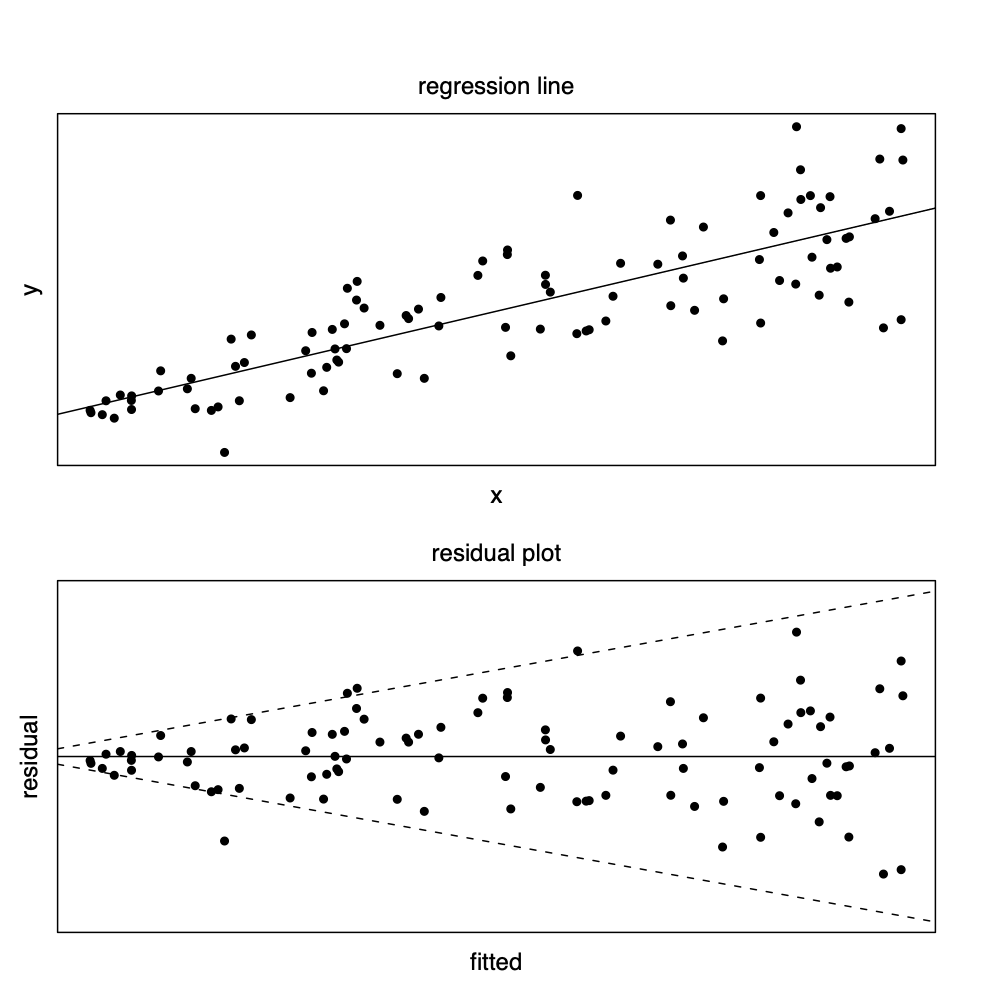
\includegraphics[width=0.8\linewidth]{hetero} \caption{오차항의 등분산성이 위반된 경우}\label{fig:hetero}
\end{figure}

\hypertarget{uxbcc0uxc218uxbcc0uxd658}{%
\section{변수변환}\label{uxbcc0uxc218uxbcc0uxd658}}

변수변환(Variable transformation)은 독립변수와 종속변수를 변환함으로서 회귀식의 적합도를 향상시켜 예측력을 높일 수 있을뿐 아니라 최소제곱법에서의 등분산성 가정에 대한 만족도를 높일 수 있는 유용한 방법이다 (variance stabilization). 이 절에서는 변수변환의 종류와 그 효과를 단순회귀식에서 살펴본다. 중회귀의 경우에는 변수변환의 적용을 복합적으로 고려해야 할 것이다.

\hypertarget{uxc9c0uxc218uxbaa8uxd615uxacfc-uxba71uxd568uxc218-uxb85cuxadf8uxbcc0uxd658}{%
\subsection{지수모형과 멱함수: 로그변환}\label{uxc9c0uxc218uxbaa8uxd615uxacfc-uxba71uxd568uxc218-uxb85cuxadf8uxbcc0uxd658}}

회귀식에 대한 모형이 지수함수 모형인 경우, 즉 독립변수와 종속변수가 다음과 같은 경우
\[ y = \beta_0 \exp (\beta_1 x) \]
종속변수에 대한 로그 변환(log transformation)을 하면 선형관계에 매우 가깝게 된다 ( \ref{fig:logtrans} ).
\[ \log(y_i) = \beta,_0 + \beta_1 x_i + e_i \]
여기서 주의할 점은 원래의 지수모형에 오차항의 지수함수가 곱해지는 형태가 되어야 로그 변환후에 등분산성의 가정을 만족하게 된다. 즉
오차항 \(e_i\)를 서로 독립이고 평균이 0, 분산이 \(\sigma^2\)이라고 하면 다음과 같은 관계가 성립된다.
\[ y_i = \beta_0 \exp (\beta_1 x_i)\exp(e_i) \quad \Rightarrow \quad \log(y_i) = \beta'_0 + \beta_1 x_i + e_i \]

\begin{figure}
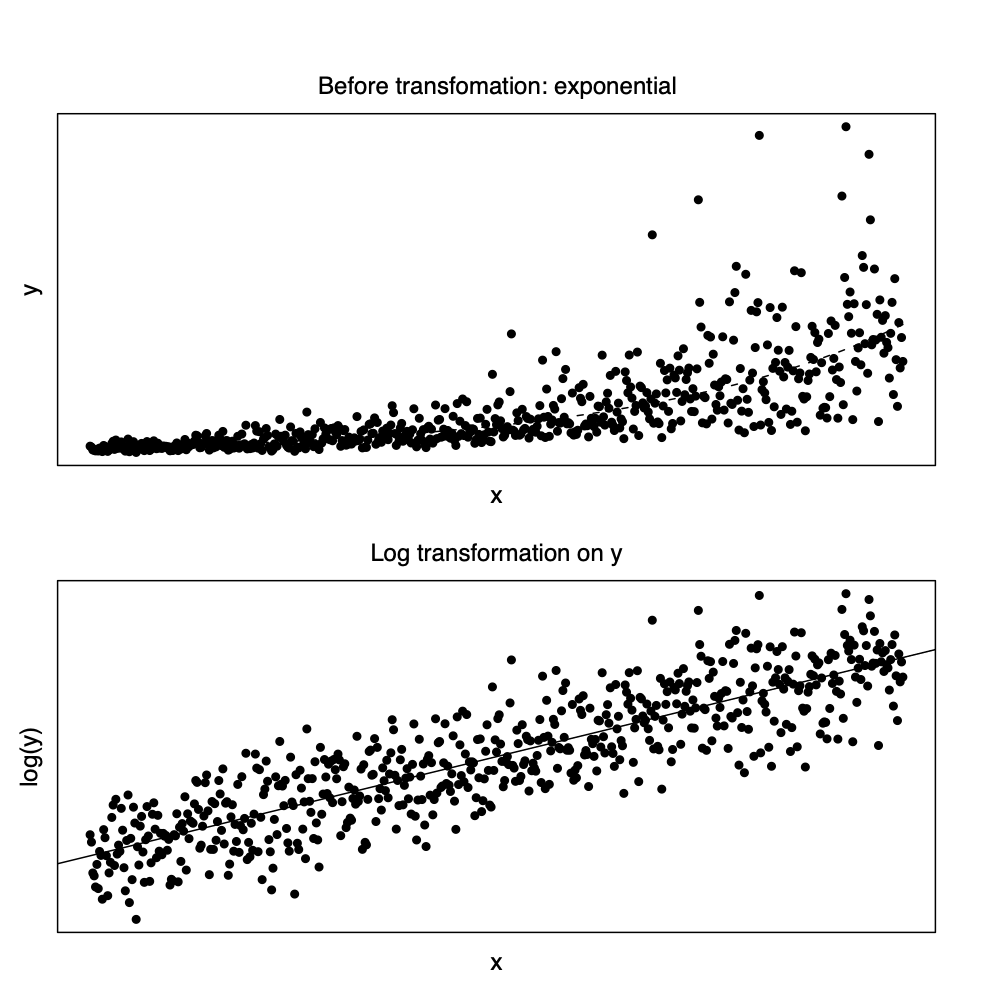
\includegraphics[width=0.8\linewidth]{logtrans} \caption{지수모형과 로그변환}\label{fig:logtrans}
\end{figure}

회귀식에 대한 모형이 멱함수모형인 경우, 즉 독립변수와 종속변수가 다음과 같은 경우
\[ y = \beta_0  x^\beta_1 \]
독립변수와 종속변수에 대한 로그 변환을 하면 선형관계에 매우 가깝게 된다.
\[ \log(y_i) = \beta,_0 + \beta_1 \log(x_i) + e_i \]
여기서 주의할 점도 원래의 멱함수모형에 오차항이 곱해지는 형태가 되어야 로그 변환후에 등분산성의 가정을 만족하게 된다. 즉
오차항 \(e_i\)를 서로 독립이고 평균이 0, 분산이 \(\sigma^2\)이라고 하면 다음과 같은 관계가 성립된다.
\[ y_i = \beta_0  x^\beta_1 \exp(e_i) \quad \Rightarrow \quad \log(y_i) = \beta'_0 + \beta_1 \log(x_i) + e_i \]

회귀식에 대한 모형이 역지수함수 모형인 경우, 즉 독립변수와 종속변수가 다음과 같은 경우
\[ y = \beta_0 \exp (\beta_1/ x) \]
종속변수에 대한 로그 변환과 독림변수에 대한 역변환을 하면 선형관계에 매우 가깝게 된다 (\ref{fig:invexp} ).
\[ \log(y_i) = \beta,_0 + \beta_1 \left ( \frac{1}{x_i} \right ) + e_i \]
여기서 주의할 점은 원래의 역지수모형에 오차항의 지수함수가 곱해지는 형태가 되어야 로그 변환후에 등분산성의 가정을 만족하게 된다.

\begin{figure}
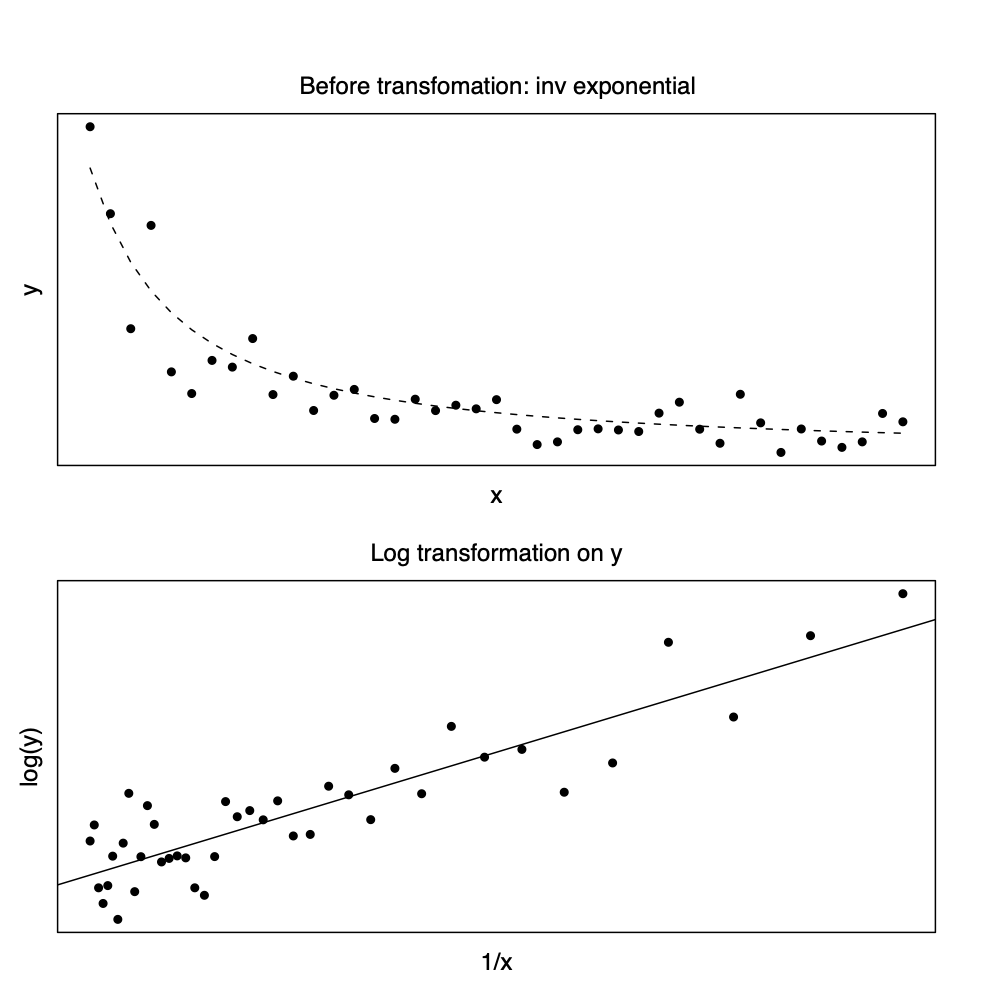
\includegraphics[width=0.8\linewidth]{invexp} \caption{역지수모형과 로그/역변환}\label{fig:invexpz}
\end{figure}

\hypertarget{uxc30duxace1uxc120uxacfc-uxc5eduxbcc0uxd658}{%
\subsection{쌍곡선과 역변환}\label{uxc30duxace1uxc120uxacfc-uxc5eduxbcc0uxd658}}

생물학, 경제학등의 문야에서 독립변수와 종속변수의 관계가 쌍곡선(Hyperbola) 형태인 경우가 많다. 독립변수가 증가함에 따라 종속변수의 값이 수렴하는 경우에 이러한 관계가 매우 유용하다.
\[ y = \frac{x}{\beta_0 + \beta_1 x} \]
이러한 경우에 독립변수와 종속변수에 모두 역변환(Inverse transformation)을 취하면 선형관계에 매우 가깝게 된다 (그림 \ref{fig:hyperbola}).
\[ \frac{1}{y_i} = \beta_0 + \beta_1 \left ( \frac{1}{x_i} \right ) + e_i \]

\begin{Shaded}
\begin{Highlighting}[]
\NormalTok{knitr}\SpecialCharTok{::}\FunctionTok{include\_graphics}\NormalTok{(}\StringTok{"hyperbola.png"}\NormalTok{)}
\end{Highlighting}
\end{Shaded}

\begin{figure}
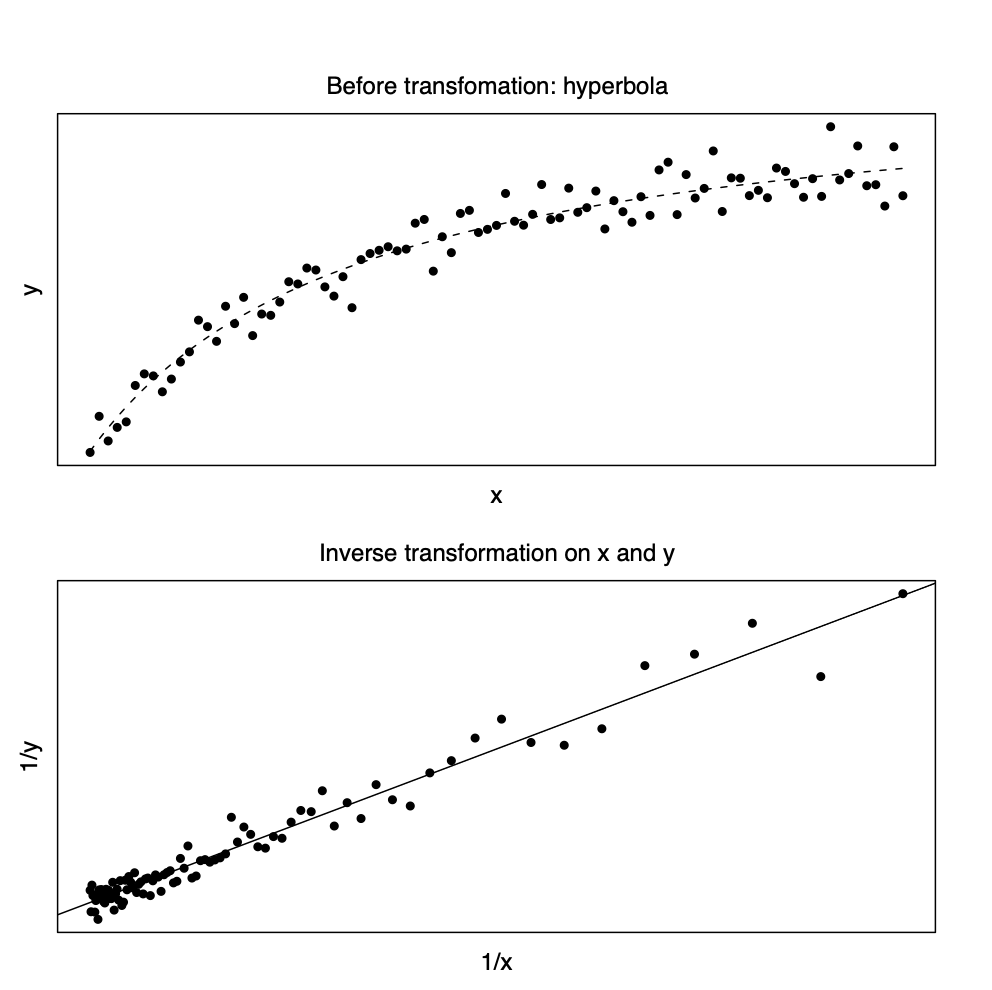
\includegraphics[width=0.8\linewidth]{hyperbola} \caption{쌍곡선과 역변환}\label{fig:hyperbola}
\end{figure}

위에서 살펴본 회귀모형들에서 변수변환후에 등분산성에 대한 가정을 만족하려면 대부분 변환전의 함수관계식에 오차항의 지수함수가 곱해지는 형태가 되어야 한다 (multiplicative error model). 이렇게 오차항이 함수관계식에 곱해지는 형태가 아니 다른 형태라면, 예를 들어 오차항이 원래의 함수관계식에 더해지는 형태 (additive error model), 등분산성의 가정이 상당히 위배될 수 있음을 주의해야 한다. 예를 들어 회귀식에 대한 모형이 지수함수 모형인 경우 서로 독립이고 평균이 0, 분산이 \(\sigma^2\)인 오차항 \(e_i\)를 함수 관계식에 더해졌다면 로그변환된 종속 변수와 독립변수는 선형관계를 보이지만 등분산성 가정은 만족하지 못하게된다 (그림 \ref{adderror}).
\[ y_i = \beta_0 \exp (\beta_1 x_i) +e_i \quad \Rightarrow \quad \log(y_i) \cong \beta'_0 + \beta_1 x_i + e^*_i \]

\begin{figure}
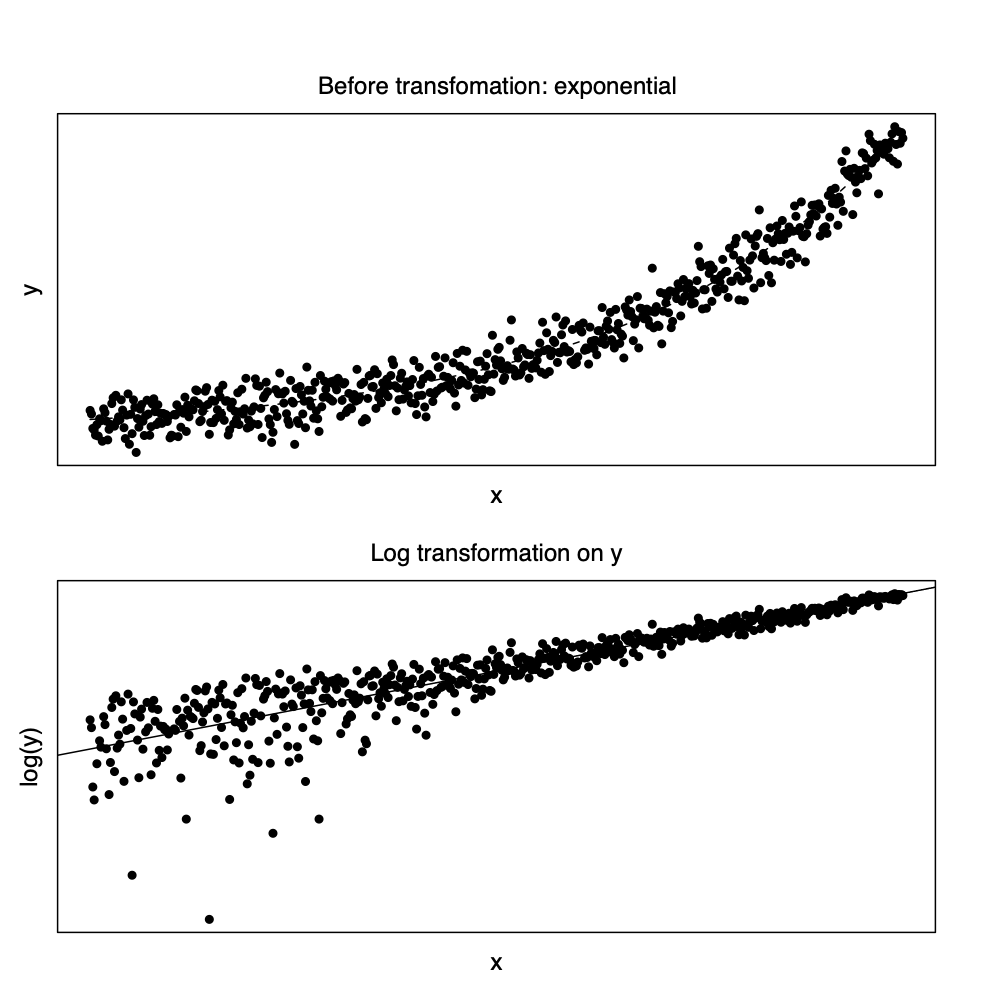
\includegraphics[width=0.8\linewidth]{adderror} \caption{Additive error model 과 로그변환}\label{fig:adderror}
\end{figure}

\hypertarget{box-cox-uxbcc0uxd658}{%
\subsection{Box-Cox 변환}\label{box-cox-uxbcc0uxd658}}

앞 절에서 보았듯이 종속변수에 로그변환 등을 적용하면 여러 가지 유용한 점이 많다. 위에서 살펴본 종속변수에 변환은 여러 가지 비선형모형을 선형모형에 가깝게 만들어 주며 Multiplicative error model과 같이 반응값이 분산이 독립변수의 크기에 영향을 받는 모형을 등분산성을 가진 형태의 모형으로 버꾸어 준다 (Variance stabilization). 이렇게 종속변수에 대한 여러 가지 변환을 하나의 체계적인 형태로 결합한것을 Box-Cox 변환으로 부르며 다음과 같아 정의한다.

\begin{equation} 
y^{(\lambda)} =
\begin{cases}
\log(y) & \text{ if } \lambda=0 \\
\frac{y^\lambda -1}{\lambda} & \text{ if } \lambda \ne 0
\end{cases}
\label{eq:boxcox}
\end{equation}

Box-Cox 변환은 로그변환과 멱변환을 모두 포함하고 있다. 또한 Box-Cox 변환된 \(y^{(\lambda)}\)가 정규분포를 따른다는 가정 하에 자료가 주어졌을때 \(\lambda\)에 대한 최대우도추정량을 구할 수 있다.

\hypertarget{uxb2e4uxc911uxacf5uxc120uxc131}{%
\section{다중공선성}\label{uxb2e4uxc911uxacf5uxc120uxc131}}

회귀분석에서 독립변수들간의 강한 선형 관계의 경향이 있을 때 이를 다중공선성(multicollinearity)라고
한다. 즉, \(p\)개의 독립변수 \(x_1,x_2,\dots,x_p\)의 관계가 다음과 같은 선형관계에 가깝다면 다중공선성이 존재한다고 한다.

\[ c_1 x_1 + c_2 x_2 + \dots + c_p x_p \cong 0 \]

다중공선성에 의해 발생하는 여러 가지 문제점들을 기술적으로 독립변수들의 강한 선형관계때문에 행렬 \(X^tX\)가 ill-conditioned 행렬이 되어 그 역행렬이 불안정하게 구해지는 결과 때문에 생기게 된다. 여기서 회귀계수의 공분산 행렬은 다음과 같이 주어짐에 유의하자.

\[ Var(\bm b) = \sigma^2 (X^t X)^{-1} \]

예를 들어서 두 개의 독립변수가 있는 회귀 모형을 생각해 보자.

\[ y = \beta_0 + \beta_1 x_1 + \beta_2 x_2 + e \]

그림 \ref{fig:multicol}에서 (a)의 경우는 두 개의 독립변수 \(x_1\)과 \(x_2\)의 관계가 독립적이어서 (linearly independent) 적합된 회귀식이(그림에서 2차원 평면) 안정적이다. 반면에 그림 \ref{fig:multicol} 에서 (b)의 경우는 두 개의 독립변수 \(x_1\)과 \(x_2\)가 완벽한 선형관계가 있기 떄문에 (linearly dependent)

\[ c_1 x_1 + c_2 x_2 = 0 \]
적합된 회귀식이 여러가지 존재한다. 이러한 경우는 매우 드물지만 \ref{fig:multicol}에서 (c)의 경우는 두 개의 독립변수 \(x_1\)과 \(x_2\)가 선형관계에 매우 가깝기 때문에 적합된 회귀식이 불안정하다.

\begin{figure}
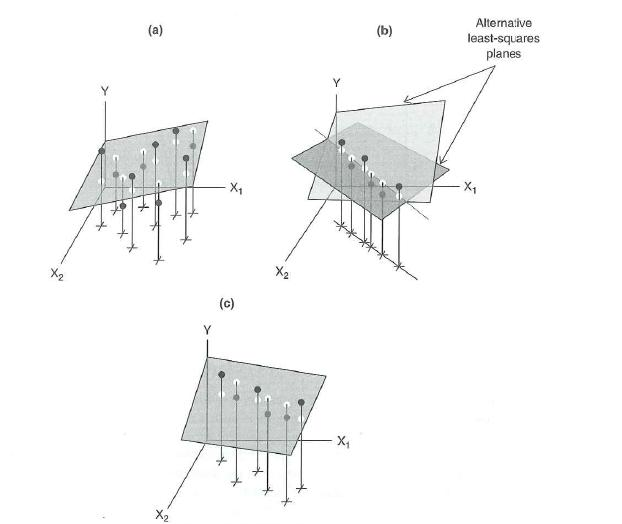
\includegraphics[width=0.8\linewidth]{multicol} \caption{회귀분석에서의 다중공선성의 정도(Fox 2008, p310)}\label{fig:multicol}
\end{figure}

회귀분석에서 다중공선성의 정도를 측정할 수 있는 통계량은 다음과 같은 것들이 있다.

\hypertarget{uxb3c5uxb9bduxbcc0uxc218uxac04uxc758-uxc0c1uxad00uxacc4uxc218}{%
\subsection{독립변수간의 상관계수}\label{uxb3c5uxb9bduxbcc0uxc218uxac04uxc758-uxc0c1uxad00uxacc4uxc218}}

독립변수간의 상관계수를 보아 강한 상관관계를 가지는 변수들이 있다면 다중공선성의 가능성이 크다.

\hypertarget{bm-xt-bm-x-uxc758-uxace0uxc720uxac12eigenvalues}{%
\subsection{\texorpdfstring{\(\bm X^t \bm X\) 의 고유값(Eigenvalues)}{\textbackslash bm X\^{}t \textbackslash bm X 의 고유값(Eigenvalues)}}\label{bm-xt-bm-x-uxc758-uxace0uxc720uxac12eigenvalues}}

행렬 \(\bm X^t \bm X\)의 고유값를 구하여 큰 순서대로 나열했을 때 가장 작은 값이 0에 매우 가까우면 다중공선성의 가능성이 크다. 만약에 독립변수들간의 선형 관계가 있다면 행렬 \(\bm X^t \bm X\)은 최대 계수(full rank) 행렬이 아니므로 하나 이상의 고유값이 0이 되게 된다.

이제 \(\lambda_1 \ge \lambda_2 \ge \dots \ge \lambda_p\)를 \(\bm X^t \bm X\)의 고유값라고 하자. 이런 가정 하에서 \(1/\lambda_i\)는 \((\bm X^t \bm X)^{-1}\)의 고유값이다. \(\bm X^t \bm X\)의 고유값에 대한 고유벡터를 \(\bm p_1, \bm p_2,\dots,\bm p_p\)라고 하고 행렬 \(\bm P=[\bm p_1, \bm p_2,\dots,\bm p_p]\)로 정의하자. 이때 다음과 같이 스펙트렇 분해를 이용하여 \(\bm X^t \bm X\)를 나타낼 수 있다.

\[ \bm P^t (\bm X^t \bm X) \bm P = \bm \Lambda = \text{diag}(\lambda_1 , \lambda_2 , \dots , \lambda_p) \]
또한

\[ (\bm X^t \bm X)^{-1} =  \bm P \bm \Lambda^{-1}\bm P^t  \]
따라서 가장 작은 고유값 \(\lambda_p\)가 매우 0에 가까우면 \((\bm X^t \bm X) \bm p_p =\lambda_p \bm p_p \approx 0\)이 성립하고 이는 \(\bm X \bm p_p \approx 0\)을 의미하여 독립변수간에 선형관계가 있다는 것을 암시한다.

일반적으로 최소제곱추정량의 공분산은 다음과 같아 나타내어지고

\[ Var(\hat {\bm \beta}) = \sigma^2 (\bm X^t \bm X)^{-1} = \sigma^2 \bm P \bm \Lambda^{-1}\bm P^t  =
\sigma^2  \sum_{i=1}^p \frac{1}{\lambda_i} \bm p_i \bm p^t_i \]

최소제곱추정량의 분산의 합(total variance)은 다음과 같다.

\[ \sum_{i=1}^p Var(\hat \beta_i) = tr[\sigma^2 (\bm X^t \bm X)^{-1}]= \sigma^2 tr[ (\bm X^t \bm X)^{-1}]=
\sigma^2 \sum_{i=1}^p \frac{1}{\lambda_i} \]

따라서 고유값의 값이 0에 가까와 지면 추정량의 분산의 합은 매우 크게 된다.

\hypertarget{uxc870uxac74uxc9c0uxc218-condition-number}{%
\subsection{조건지수 (condition number)}\label{uxc870uxac74uxc9c0uxc218-condition-number}}

다중공선성의 판별을 위하여 행렬 \(\bm X^t \bm X\)의 고유값이 중요한 측도라고 했다. 고유값을 상대적으로 비교하면 다중공선성을 더 명확하게 알 수 있다.
조건지수는 가장 튼 고유값과 다른 고유값의 비율의 제곱근으로 나타내어진다.

\[ \kappa_i = \sqrt{\frac {\lambda_1}{\lambda_i}}, \quad i=2,3,\cdots,p \]

중요한 역활을 하는 조건지수는 가장 작은 고유값에 의한 것이다.

\[ \kappa_p =\kappa(\bm X) = \sqrt{\frac {\lambda_1}{\lambda_p}} \]

\(\kappa(\bm X)\)의 값이 크면 ㅌ클수록 다중공선성의 가능성이 높다. 일반적으로 \(\kappa(\bm X)\) 가 30 이상이면 다중공선성의 가능성이 크다고 본다.

\hypertarget{uxbd84uxc0b0uxd33duxcc3duxacc4uxc218-variance-inflation-factor-vif}{%
\subsection{분산팽창계수 (Variance Inflation Factor ;VIF)}\label{uxbd84uxc0b0uxd33duxcc3duxacc4uxc218-variance-inflation-factor-vif}}

하나의 독립변수 \(x_i\)를 나머지 다른 \(p-1\)개의 독립변수 \(x_1,\dots, x_{i-1}, x_{i+1},\dots, x_p\)를 이용하여 회귀식을 적합시킬 수 있다. 이때 다중공선성이 존재한다면 적합된 회귀식의 결정계수 \(R^2_i\)는 1에 매우 가까울 것이다

\[ x_i = \beta_0 + \beta_1 x_1 + \dots + \beta_{i-1} x_{i-1} +\beta_{i+1} x_{i+1} + \dots + \beta_p x_p +e \]

이때 독립변수 \(x_i\)에 대한 VIF는 다음과 같이 정의되며 그 값이 5 또는 10보다 크면 다중공선성의 가능성이 크다.

\[ VIF_i = \frac{1}{1-R_i^2} \]

\hypertarget{compute}{%
\chapter{계산 방법}\label{compute}}

이제 선형모형에서 회귀게수를 구하는 계산 방법에 대하여 알아보자. 최소제곱법(동시에 최대 가능도 추정법)에 의한 회귀게수의 추정치를 구하려면 다음과 같은 최적화 문제를 풀어야한다.

\begin{equation}
\underset{\bm \beta}{\min} \norm{ \bm y - \bm X \bm \beta}^2 
\label{eq:comp-crit}
\end{equation}

위의 최적화 문제로 부터 유도된 회귀계수에 대항 정규 방정식(normal equation)은 다음과 같다.

\begin{equation}
 {\bm X}^t \bm X \bm \beta = \bm X^t \bm y
\label{eq:comp-lse}
\end{equation}

식 \eqref{eq:comp-lse} 에 대한 해를 구하는 경우 대수적으로는 \(\hat { \bm \beta} = ({\bm X}^t \bm X )^{-1} \bm X^t \bm y\)로 표시하지만
실제 계산에서 역행렬 \(({\bm X}^t \bm X )^{-1}\)을 실제로 구하지는 않는다. 식 \eqref{eq:comp-lse}에서 나타난 것과 같은 선형방정식을
푸는 계산적 방법은 가우스 소거법(Gauss elimination ), 교환 연산(sweep operator) 등에 의한 전통적인 방법들이 있다. 교환 연산(sweep operator) 방법은 SAS 프로그램에서 최소제곱법을 푸는 방법으로 사용된다. 이러한 전통적인 방법들은 가우스 소거법에 근거하여 핼과 열 연산에 의한 소거법을 기반으로 한다. 하지만 최근에 나온 통계 계산 패키지에서는 소거법을 사용하지 않는다.

이 장에서는 최근 통계 계산 프로그램이 사용하는 행렬 분해에 의한 방법을 살펴보고자 한다. 다음에 나오는 방법들은 계획행렬 \(\bm X\)가 최대 계수(full rank)가 아닌 경우에도 적용할 수 있지만 여기서는 최대 계수인 경우만 고려하겠다.

\hypertarget{uxcd10uxb808uxc2a4uxd0a4-uxbd84uxd574}{%
\section{촐레스키 분해}\label{uxcd10uxb808uxc2a4uxd0a4-uxbd84uxd574}}

방정식 \eqref{eq:comp-lse} 에서 외쪽 항에 있는 \(\bm A = {\bm X}^t \bm X\) 는 양정치 행렬이다. 양정치 행렬 A은 다음과 같이 유일하게 촐레스키 분해(CHolesky decomposition)가 가능하다.

\begin{equation}
\bm A = {\bm X}^t \bm X = \bm L \bm L^t 
\label{eq:comp-chol}
\end{equation}

위의 분해에서 행렬 \(\bm L\)은 양수의 대각원소를 가지는 하삼각 행렬(lower triangular matrix)이다.

이제 촐레스키 분해를 정규 방정식에 적용해보자.

\[   \bm L \bm L^t \bm \beta = \bm X^t \bm y \]

위의 식에서 \(\bm L^t \bm \beta = \bm \beta_*\)라고 하면 다음과 같은 방정식을 얻게 되고 이 방정식은 행렬 \(\bm L\)이 하삼각 행렬이기 때문에 대수적으로 축차식을 이용하여 쉽게 해 \(\hat {\bm \beta}_*\)를 얻을 수 있다.

\[ \bm L \bm \beta_* = \bm X^t \bm y \]

다음으로 관계식 \(\bm L^t \bm \beta = \bm \beta_*\) 이용하여 다음의 방정식을 풀면 회귀계수의 추정치 \(\hat { \bm \beta}\)를 얻게 된다. 아래의 방정식 또한 \(\bm L^t\)가 상삼각 행렬이기 때문에 축차적인 계산이 가능하다.

\[ \bm L^t \bm \beta = \hat {\bm \beta}_*\]

\hypertarget{qr-uxbd84uxd574}{%
\section{QR 분해}\label{qr-uxbd84uxd574}}

계획 행렬 \(\bm X\)의 QR 분해가 다음과 같이 주어졌다고 하자. \(rank(\bm X)=p< n\) 이라고 가정하자.

\[  \bm X =\bm Q_1 \bm R \]
위의 QR 분해에서 \(\bm Q_1\)는 \(p\) 개의 직교하는 열을 가진 \(n \times p\) 행렬이다 (\(\bm Q_1^t \bm Q_1= \bm I\)). 또한 행열 \(\bm R\)은 차원이 \(p \times p\)인 상삼각 행렬(upper diagonal matrix)이다.

그러면 행렬 \(\bm X\)는 다음과 같은 확장된 분해를 가진다.

\begin{equation*}
\bm  X = \bm Q \bm R =  
\begin{bmatrix} \bm Q_1 & \bm Q_2  \end{bmatrix} \begin{bmatrix} \bm R \\ \bm 0 
\end{bmatrix} 
\end{equation*}

위에서 \(\bm Q_2\) 는 행렬 \(\bm Q_1\)의 열들과 직교하는 \(n-p\) 개의 추가 정규직교 벡터들로 이루어진 행렬이다. \(\bm Q_1\)과 \(\bm Q_2\)는 각각 \(n \times p\), \(n \times (n-p)\)의 행렬이다. 따라서 행렬 \(\bm Q = [\bm Q_1 ~\bm Q_2]\)는 \(n \times n\) 직교행렬이다 (\(\bm Q^t \bm Q = \bm Q \bm Q^t = \bm I\)).

또한 \(\bm R\)는 \(p \times p\) 상삼각행렬고 \(\bm 0\)은 차원이 \((n-p) \times p\)인 영행렬이다.

이제 \(\bm Q^t \bm Q =\bm I\)를 이용하여 잔차제곱합 \(\norm{ \bm y-\bm X \bm \beta}^2\)를 다음과 같이 분해할 수 있다.

\begin{align*}
\norm{ \bm y-\bm X \bm \beta}^2 & = (\bm y-\bm X \bm \beta)^t (\bm y-\bm X\bm \beta) \notag \\
  & =(\bm y-\bm X \bm \beta)^t \bm Q \bm Q^t (\bm y-\bm X \bm \beta) \notag \\
  & = (\bm Q^t \bm y-\bm Q^t \bm X \bm \beta)^t  (\bm Q^t  \bm y-\bm Q^t  \bm X \bm \beta) \notag \\
  & =(\bm c -\bm R \bm \beta)^t  (\bm c -\bm R \bm \beta) \notag \\
  & =  
  \left ( 
  \begin{bmatrix}
  \bm c_1 \\
  \bm c_2
  \end{bmatrix}
  -
  \begin{bmatrix}
  \bm R \\
  \bm 0
  \end{bmatrix}
  \bm \beta
  \right )^t
   \left ( 
  \begin{bmatrix}
  \bm c_1 \\
  \bm c_2
  \end{bmatrix}
  -
  \begin{bmatrix}
  \bm R \\
  \bm 0
  \end{bmatrix}
  \bm \beta
  \right ) \notag \\
  & = (\bm c_1 -\bm R \bm \beta)^t  (\bm c_1 -\bm R \bm \beta) + \bm c_2^t \bm c_2 \notag \\
  & = \norm{ \bm c_1 - \bm R \bm \beta }^2 + \norm{\bm c_2}^2 
\end{align*}

결과를 요약하면 다음과 같은 분해를 얻는다.

\begin{equation}
\norm{ \bm y-\bm X \bm \beta}^2 = \norm{ \bm c_1 - \bm R \bm \beta }^2 + \norm{\bm c_2}^2 
\label{eq:decompres}
\end{equation}

여기서

\[
\bm c= \bm Q^t \bm y=
 \begin{bmatrix} 
   \bm Q_1^t \\ 
   \bm Q_2^t 
   \end{bmatrix} \bm y 
   =
   \begin{bmatrix} 
   \bm Q_1^t \bm y  \\ 
   \bm Q_2^t \bm y 
   \end{bmatrix}
   = \begin{bmatrix} 
   \bm c_1 \\ 
   \bm c_2 
\end{bmatrix}  
\]

위의 식 \eqref{eq:decompres}를 보면 벡터 \(\bm c_2= \bm Q_2^t \bm y\)는 \(\bm \beta\)와 관계가 없으므로 잔차제곱합 \(\norm{ \bm y-\bm X \bm \beta}^2\) 을 최소화하는
\(\bm \beta\)는 \(\norm{ \bm c_1 - \bm R \bm \beta }^2\)을 0으로 만드는 것이다. 즉 \(\bm R \bm \beta =\bm c_1\)를 만족하는 \(\bm \beta\)가 최소제곱 추정량이다.

\[
\min_{\bm \beta} \norm{ \bm y-\bm X \bm \beta}^2 = \min_{\bm \beta} \norm{ \bm c_1 - \bm R \bm \beta }^2 +  \norm{\bm c_2}^2 
\]

\(\bm X\)가 완전계수 행렬이므로 상삼각행렬인 \(\bm R\)도 완전계수이다. 따라서 방정식 \(\bm R \bm \beta = \bm c_1\)는 유일한 해는 상삼각행렬의 성질을 이용하여 축차식으로 쉽게 구할 수 있다.

\[ \hat {\bm \beta} =\bm R^{-1} \bm c_1 \]

위의 추정량은 실제 역행렬을 구하지 않고 QR 분해를 이용하여 회귀계수를 구하는 방법 중에 하나이다.

참고로 잔차제곱합 \(SSE\)는 다음과 같이 계산된다.

\[ SSE = \norm{ \bm y-\bm X \hat {\bm \beta}}^2 = \norm{\bm c_2}^2 = \bm y^t \bm Q_2 \bm Q_2^t \bm y \]

\begin{rmdnote}
QR 분해에 대한 자세한 내용은 \href{https://ilovedata.github.io/teaching/matrix1/qr.pdf}{여기}를 참조하시오
\end{rmdnote}

\hypertarget{svd}{%
\section{SVD}\label{svd}}

이제 최소제곱법을 SVD (Singular Value Decomposition) 으로 푸는 방법을 살펴보자. \(rank(\bm X)=p< n\) 이라고 가정하자.

이제 게획행렬은 SVD 를 이용하여 다음과 같이 분해할 수 있다.

\[  \bm X = \bm U \bm R  \bm V^t\]
위의 분해에서 각 행렬의 특성은 다음과 같다.

\begin{itemize}
\tightlist
\item
  \(\bm U\): \(n \times n\) 직교행렬
\item
  \(\bm V\): \(p \times p\) 직교행렬
\end{itemize}

\(\bm R\)은 \(n \times p\) 행렬이며 윗 부분 \(p \times p\) 행렬 \(R_1\)은 대각 행렬이다.
\(\bm R\)의 아래 부분 \((n-p) \times p\)는 영행렬이다.

\[ 
\bm R = 
\begin{bmatrix}
\bm R_1 \\
\bm 0
\end{bmatrix}
\quad 
\bm R_1 = diag(r_1, r_2, \dots, r_p)
\]

따라서 계획행렬의 분해는 다음과 같이 축소할 수 있다.

\begin{equation}
\bm X = \bm U \bm R  \bm V^t = 
\begin{bmatrix}
\bm U_1 & \bm U_2
\end{bmatrix}
\begin{bmatrix}
\bm R_1 \\
\bm 0
\end{bmatrix}
\bm V^t
= \bm U_1 \bm R_1  \bm V^t
\label{eq:svd}
\end{equation}

위의 식 \eqref{eq:svd} 에서 행렬 \(\bm U_1\)은 \(n \times p\), \(\bm U_2\)은 \(n \times (n-p)\) 행렬이며
\(\bm U_1^t \bm U_1 = \bm 0\), \(\bm U_2^t \bm U_2 = \bm I\) 이다.

이제 최소제곱법의 해를 SVD 로 구해보자.

\begin{align*}
\norm{ \bm y-\bm X \bm \beta}^2 & = (\bm y-\bm X \bm \beta)^t (\bm y-\bm X\bm \beta) \\
  & = (\bm y-\bm U  \bm R   \bm V^t \bm \beta)^t (\bm y-\bm U  \bm R   \bm V^t \bm \beta) \\
  & =  (\bm y-\bm U  \bm R   \bm V^t \bm \beta)^t \bm U   \bm U ^t (\bm y-\bm U  \bm R   \bm V^t \bm \beta) \\
  & =  (\bm U ^t \bm y- \bm U ^t \bm U  \bm R   \bm V^t \bm \beta)^t    (\bm U ^t \bm y-\bm U ^t \bm U  \bm R   \bm V^t \bm \beta) \\
  & =  (\bm U ^t \bm y-  \bm R   \bm V^t \bm \beta)^t    (\bm U ^t \bm y- \bm R   \bm V^t \bm \beta) \\
  & = \norm{ \bm U ^t \bm y-  \bm R   \bm V^t \bm \beta}^2 \\
  & = \norm{ \bm c -  \bm R   \bm \beta_*}^2  \\
    & =  
  \left ( 
  \begin{bmatrix}
  \bm c_1 \\
  \bm c_2
  \end{bmatrix}
  -
  \begin{bmatrix}
  \bm R_1 \\
  \bm 0
  \end{bmatrix}
  \bm \beta_*
  \right )^t
   \left ( 
  \begin{bmatrix}
  \bm c_1 \\
  \bm c_2
  \end{bmatrix}
  -
  \begin{bmatrix}
  \bm R_1 \\
  \bm 0
  \end{bmatrix}
  \bm \beta_*
  \right )  \\
& =  (\bm c_1 -\bm R_1 \bm \beta_*)^t  (\bm c_1 -\bm R_1 \bm \beta_*) + \bm c_2^t \bm c_2  \\
  & = \norm{ \bm c_1 - \bm R_1 \bm \beta_* }^2 + \norm{\bm c_2}^2 
\end{align*}

이제 위의 분해에서 다음과 같이 새로운 벡터를 정의한다.

\begin{equation}
\bm c = \bm U^t \bm y,  \quad \bm \beta_* = \bm V^t \bm \beta 
\label{eq:svdpara}
\end{equation}

그리고

\[
\bm c= \bm U^t \bm y=
 \begin{bmatrix} 
   \bm U_1^t \\ 
   \bm U_2^t 
   \end{bmatrix} \bm y 
   =
   \begin{bmatrix} 
   \bm U_1^t \bm y  \\ 
   \bm U_2^t \bm y 
   \end{bmatrix}
   = \begin{bmatrix} 
   \bm c_1 \\ 
   \bm c_2 
\end{bmatrix}  
\]

이제 QR 분해와 유사하게 최소제곱의 오차제곱합은 다음과 같이 분해된다.

\begin{equation}
\norm{ \bm y-\bm X \bm \beta}^2  = 
\norm{ \bm c_1 - \bm R_1 \bm \beta_* }^2 + \norm{\bm c_2}^2 
 =\sum_{i=1}^p (c_{1i} - r_i \beta_{*i})^2 + \norm{\bm c_2}^2 
\label{eq:svdlse}
\end{equation}

위의 분해 \eqref{eq:svdlse} 는 행렬 \(\bm R_1\)이 대각행렬임을 이용한 것이다. 이제 식 \eqref{eq:svdlse} 를 최소하하는 해
\(\hat {\bm \beta}_*\) 는 다음과 같이 구할 수 있고

\[ \hat \beta_{*i} =\frac{ c_{1i}}{r_i} \]

최종적으로 식 \eqref{eq:svdpara} 의 관계를 이용하면 최소제곱 추정량은 다음과 같이 주어진다.

\[ \hat {\bm \beta} = \bm V \hat {\bm \beta}_* \]
참고로 QR 분해 방법과 유사하게 잔차제곱합 \(SSE\)는 다음과 같이 계산된다.

\[ SSE = \norm{ \bm y-\bm X \hat {\bm \beta}}^2 = \norm{\bm c_2}^2 = \bm y^t \bm U_2 \bm U_2^t \bm y \]

\begin{rmdnote}
위에서 논의한 촐레스키, QR, SVD 를 이용한 최소제곱 추정량 \(\hat \beta\)를 구하는 방법은 계획행렬이
완전 계수가 아닌 경우에도 (\(rank(X)<p\)) 쉽게 적용할 수 있다.
\end{rmdnote}

\hypertarget{residual}{%
\chapter{관측값에 대한 진단}\label{residual}}

\hypertarget{uxc11cuxb860}{%
\section{서론}\label{uxc11cuxb860}}

회귀분석을 포함한 통계적 자료분석에서 흔하게 접하는 문제는 자료 중의
일부가 통계적 모형에 의해 추정된 평균적인 경향에서 매우 벗어나 있는 점을
발견하게 되는 경우이다.

이러한 경우 평균적인 경향에서 매우 벗어난 자료를 분석에서 제외시킬
것인지에 대한 논의도 필요할 수 있으며 이러한 자료들이 모형의 모수에 대한
추정에 어떤 영향을 미칠 것인자에 대한 검토도 필요할 수 있다.

평균적인 경향에서 매우 벗어난 자료를 흔히 이상점(outlier)라고 부른다.
회귀분석에서 이러한 이상점은 회귀계수 추정과 그에 따른 여러 가지 통계적
추론에 많은 영향을 미친다. 따라서 이상점들이 회귀분석의 계수 추정에 어떤
영향을 얼만큼 끼치는가에 대한 검토는 매우 중요하다.

\hypertarget{uxc774uxc0c1uxc810uxc758-uxc720uxd615}{%
\section{이상점의 유형}\label{uxc774uxc0c1uxc810uxc758-uxc720uxd615}}

일차원 자료에서는 평균적인 경향에서 매우 벗어난 자료의 식별이 단순하고
쉽다. 예를 들어 다음과 같이 일변량 자료 \(\bm x\)만 고려하면 이상점이 어떤
점인지는 쉽게 찾을 수 있다.

\[ \bm x^t = (1,2,3,4,5,10) \]

그러나 반응변수와 독립변수들을 고려해야 하는 회귀분석에서 이상점은
간단하게 파악하기 힘들고 상황에 따라 그 의미가 매우 다르다.

회귀분석에서 이상점의 다양한 종류와 그 영향을 알아보기 위하여
단순회귀분석을 고려하고 다음 그림을 보자.

\begin{figure}
\centering
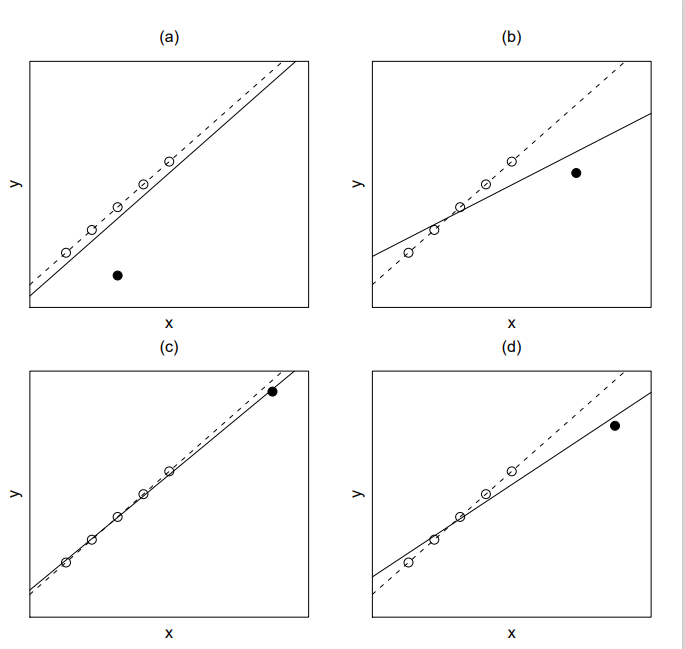
\includegraphics{outliers.png}
\caption{여러가지 종류의 이상점과 그 영향}
\end{figure}

위의 그림에서 실선은 검정색 점을 포함해서 적합한 회귀직선이고 점선은
검정색 점을 제외했을 때의 회귀직선이다

그림의 (a)에서 검정색 점은 설명변수 \(x\)에 대해서는 이상점이 아니지만
\(x\)가 주어진 경우 반응변수 \(y\)에 대해서는 평균적인 경향에서 많이 벗어나
있기 때문에 이상점이다. 이러한 이상점을 회귀이상점(regression
outlier)라고 부르기도 한다. (a)의 회귀이상점의 유무는 회귀계수의 추정에
크게 영향을 주지 않는다. 이렇게 어떤 관측점이 있고 없음에 따라
회귀계수의 값이 크게 변하지 않는다면 그 자료의 영향력(leverage)이 작다고
한다.

(b)에서의 검은 점은 설명변수 \(x\)에 대하여 이상점이며 또한
회귀이상점이다. 더 나아가 이 이상점을 제외하고 적합한 회귀계수는
이상점을 포함했을 때 적합한 회귀계수와 매우 다르다. 이 경우 이 이상점은
큰 영향력을 가졌다고 말한다.

(c)에서의 검은 점은 설명변수 \(x\)에 대해서 이상점이지만 회귀이상점은
아니다. 이러한 경우 이상점의 유무에 따라 회귀계수의 값이 크게 변하지
않으므로 이상점은 작은 영향력을 가졌다고 말한다. 하지만 (c)에서의 검은
점이 설명변수 \(x\)의 중심점으로부터 크게 멀어져있으므로 \(y\)의 값이 조그만
변해도 그림 (d)와 같이 큰 영향력을 가진다.

관측치 \(y_i\) 를 제외할 때와 포함할 때의 회귀계수 추정치가 매우 다르면 그
관측치를 영향점(influential point)라고 하며 그 영향의 크기는 그 점이
가진 영향력(leverage)의 크기와 평균에서 떨어진 정도에 비례한다.

\begin{rmdimportant}
자료가 선형모형의 계수 추정에 미치는 영향 \(\propto\) 영향력의 크기 \(\times\) 이상치의 특이한 정도
\end{rmdimportant}

위에서 살펴보았듯이 회귀분석에서 이상점의 종류와 그 영향은 매우 다양하며
복잡하다. 이러한 이상점의 종류와 회귀계수의 영향에 대하여 분석할 때
유용하게 쓰이는 통계량이 잔차(residual)이다.

\hypertarget{uxc9c0uxb81buxac12}{%
\section{지렛값}\label{uxc9c0uxb81buxac12}}

\(y\)가 반응변수이고 \(p-1\)개의 설명변수 \(x_1,x_2,\dots,x_{p-1}\)가 있을 때
회귀식은 다음과 같이 표현된다.

\[ \bm y = \bm X \bm \beta + \bm e \]

회귀계수 \(\bm \beta\)의 최소제곱 추정치 \(\hat{ \bm \beta}\)는 다음과 같이
주어지며

\[ \hat{ \bm \beta} = (\bm X^t \bm X)^{-1} \bm X^t \bm y \]

관측값 \(\bm y\) 의 추정치 \(\hat {\bm y}\)는 다음과 같다.

\[  \hat {\bm y} = \bm X \hat{ \bm \beta} =  \bm X (\bm X^t \bm X)^{-1} \bm X^t \bm y \equiv \bm H \bm y \]

여기서 \(\bm H= \bm X (\bm X^t \bm X)^{-1} \bm X^t\)를 사영행렬(hat matrix
또는 projection matrix)라고 부르며 사영행렬 \(\bm H\) 의 \(i\) 번째
대각원소를 \(h_{ii}\)라고 하며 이는 이상치 또는 영향치 분석에 중요한
역할을 한다.

\(i\)번째 관측치의 설명변수 벡터를 다음과 같이 표시하면

\[\bm x_{i}^t=(1, x_{i1},x_{i2},\dots, x_{i,p-1}) \]

\(\bm H\) 의 \(i\) 번째 대각원소를 \(h_{ii}\)는 다음과 같이 표현된다.

\begin{equation}
 h_{ii} = \bm x_{i}^t (\bm X^t \bm X)^{-1}  \bm x_{i} 
\label{eq:hii}
\end{equation}

\(h_{ii}\)는 \(i\) 번째 관측치의 설명변수 \((x_{i1},x_{i2},\dots, x_{i,p-1})\)
들이 모든 관측치의 평균 \((\bar x_1, \bar x_2,\dots, \bar x_{p-1})\) 에서
얼마나 멀리 떨어져 있는가에 대한 상대적인 양을 나타낸다. 따라서 \(h_{ii}\)
를 지렛점(leverage point)라고 부른다.

지렛점 값이 클수로 영향점일 가능성이 크며 큰 값을 높은 지렛값(high
leverage point)라고 부른다.

보통 \(h_{ii}\)값이 \(p/n\)보다 크면 영향력이 크다고 말한다. 참고로 단순
회귀식에서 \(h_{ii}\)는 다음과 같이 주어진다.

\[ h_{ii} = \frac{1}{n} + \frac{ ( x_i-\bar x)^2 }{\sum (x_i-\bar x)^2} \]

또한 \(h_{ii}\)값을 모두 더하면 설명변수의 개수와 같다.
\[ tr(\bm H)=\sum_{i=1}^k h_{ii} = p \]

\hypertarget{uxb0b4-uxd45cuxc900uxd654-uxc794uxcc28}{%
\section{내 표준화 잔차}\label{uxb0b4-uxd45cuxc900uxd654-uxc794uxcc28}}

잔차 \(r_i\)는 \(y\) 의 실제 관측값과 그 추정치의 차이이며

\begin{equation}
r_i = y_i -\hat y_i  = y_i - {\bm x}_i^t \hat {\bm \beta}
\label{eq:resid}
\end{equation}

잔차벡터에 대한 식은 다음과 같다.

\begin{equation}
\bm r = \bm y - \hat {\bm y} = \bm y - \bm H \bm y = (\bm I-\bm H)\bm y 
\label{eq:residvec}
\end{equation}

잔차의 공분산 행렬을 살펴보면 다음과 같이 주어진다. 따라서 \(i\) 번째
잔차의 분산은 \(Var(r_i) = (1-h_{ii})\sigma^2\) 이다.

\begin{equation}
Var(\bm r) = \sigma^2 (\bm I-\bm H) 
\label{eq:residvar}
\end{equation}

위에서 언급한 잔차 \(r_i\) 를 보통 잔차(ordinary residual)이라고 하며 그
크기가 단위에 따라 바뀌므로 잔차분석에서는 표준화 잔차(standardized
residual)을 더 많이 사용한다.

아래와 같이 잔차를 그 표준편차로 나눈 값을 \textbf{내 표준화 잔차(internally
studentized residual)} 이라고 부른다.

\begin{equation}
r^s_i = \frac{r_i}{s \sqrt{1-h_{ii}}} 
\label{eq:residinternal}
\end{equation}

위의 식에서 \(s\)는 오차항의 표준편차 \(\sigma\)의 추정량이며 \(h_{ii}\)는
사영행렬 \(\bm H\) 의 \(i\) 번째 대각원소(즉 지렛값)이다.

잔차분석에서는 척도(scale)에 영향이 없는 표준화 잔차를 이용하는 것이
좋다. 그 값이 클수로 이상치일 가능성이 크다. 보통 내표준화 잔차의
절대값이 2보다 크면 이상치일 가능성이 크다.

\hypertarget{uxad00uxce21uxac12uxc758-uxc601uxd5a5-uxacc4uxc218-uxcd94uxc815}{%
\section{관측값의 영향: 계수 추정}\label{uxad00uxce21uxac12uxc758-uxc601uxd5a5-uxacc4uxc218-uxcd94uxc815}}

회귀분석에서 하나의 관측치가 회귀계수의 추정에 영향을 미치는 정도를
알아볼 때 유용한 방법은 그 관측치를 제외했을 때의 최소제곱추정량과
포함했을 때의 추정량을 비교하는 것이다.

\(i\)번째 관측치에 대한 반응값과 설명변수들이 다음과 같은 때

\[ y_i, \quad \bm x_{i}^t=(1, x_{i1},x_{i2},\dots, x_{i,p-1}) \]

\(i\)번째 관측치를 제외한 자료에서 반응변수와 설명변수의 벡터식을 다음과
같이 표시한다.

\[ \bm y_{-i}, \quad \bm X_{-i} \]

\(i\)번째 관측치를 제외했을 때 회귀계수의 최소제곱추정량을
\(\hat{ \bm \beta}_{-i}\)라 하면 모든 관측치를 이용한 최소제곱추정량을
\(\hat{ \bm \beta}\)와의 관계는 다음과 같이 나타낼 수 있다. 아래 식 세번째
중의 결과는 \ref{matrixalgebra}의 우드베리 공식을 이용하였다.

\begin{align}
\hat{ \bm \beta}_{-i} & =  (\bm X_{-i}^t \bm X_{-i})^{-1} \bm X_{-i}^t \bm y_{-i}\\
& = (\bm X^t \bm X - \bm x_{i} \bm x_{i}^t)^{-1} (\bm X^t \bm y -  \bm x_{i} y_{i}) \\
& = \left [ (\bm X^t \bm X)^{-1} - \frac { (\bm X^t \bm X)^{-1}  \bm x_{i} \bm x_{i}^t
  (\bm X^t \bm X)^{-1}  }{ 1- \bm x_{i}^t (\bm X^t \bm X)^{-1}  \bm x_{i} } \right ]
(\bm X^t \bm y -  \bm x_{i} y_{i})  \\
& = \hat{ \bm \beta} + \frac{1}{1-h_{ii}} (\bm X^t \bm X)^{-1}  \bm x_i \left [ \bm x_i^t \hat{ \bm \beta} - (1-h_{ii}) y_i - h_{ii} y_i \right ] \\
& =  \hat{ \bm \beta} - \frac{1}{1-h_{ii}} (\bm X^t \bm X)^{-1}  \bm x_i ( y_i - \bm x_i^t \hat{ \bm \beta}) \\
& =  \hat{ \bm \beta} - \frac{r_i}{1-h_{ii}} (\bm X^t \bm X)^{-1}  \bm x_i 
\label{eq:betaminusi}
\end{align}

또한 \(i\)번째 관측치를 제외했을 때 오차항 분산의 추정량을 \(s^2_{-i}\)로
나타낸다.

\begin{equation}
 s^2_{-i} = \frac{1}{n-p-1} \sum_{j \ne i} (y_j - {\bm x}_j^t \hat{ \bm \beta}_{-i} )^2 
\label{eq:s2minusi}
\end{equation}

\hypertarget{uxc678-uxd45cuxc900uxd654-uxc794uxcc28uxc640-press-uxc794uxcc28}{%
\section{외 표준화 잔차와 PRESS 잔차}\label{uxc678-uxd45cuxc900uxd654-uxc794uxcc28uxc640-press-uxc794uxcc28}}

잔차를 표준화 할 떄 \(i\)번째 관측치를 제외했을 때 분산의 추정량을
\(s^2_{-i}\)을 이용하는 것이 합리적이다. 이는 반응값이 이상점인 경우
분산의 추정량이 커지게 된다. 식 \eqref{eq:residinternal}에서 정의된 내
표준화 잔차에서는 이상점이 분산의 추정량에 영향을 주어 잔차의 크기가
작아지게 된다. 따라서 내 표본화 잔차는 이상점을 구별할 수 있는 능력이
떨어진다. 이러한 점을 보완하기 위하여 이상점의 영향을 약화시킬 수 있도록
\(s^2_{-i}\)를 이용하여 표준화 한 양이 아래와 같이 정의된 표준화 잔차이다.

\begin{equation}
r^*_i = \frac{r_i}{s_{-i} \sqrt{1-h_{ii}}} 
\label{eq:residexternal}
\end{equation}

식 \eqref{eq:residexternal}에서 정의된 차를 표준화 잔차(studentized
residual) 또는 \textbf{외 표준화 잔차(externally studentized residual)}라고
부른다.

외 표준화 잔차는 \(i\)번째 관측치가 회귀식 적합에 미치는 영향을 내 표분화
잔차보다 더 민감하게 탐색할 수 있다. 보통 외 표준화 잔차의 절대값이
2보다 크면 이상치일 가능성이 크다.

\textbf{PRESS 잔차} \(r_{i,-i}\)는 \(i\) 번쨰 관측값을 빼고 적합한 회귀식으로
부터 얻은 \(E(y| \bm x_i)\)의 추정치 \(\hat y_{i,-i}\)를 이용하여 만든
잔차이다. PRESS 잔차는 다음과 같이 정의된다.

\begin{equation}
r_{i,-i}  =   y_i - \hat y_{i,-i} = y_i - \bm x^t_i \hat{ \bm \beta}_{-i} 
\label{eq:residpress}
\end{equation}

실제 PRESS 잔차를 구할 경우 관측값을 제외하지 않고도 원래의 회귀식을
이용하여 아래와 같이 쉽게 구할 수 있다. 그 값이 클수로 이상치 또는
영향점일 가능성이 크다.

\begin{align}
r_{i,-i} & =   y_i - \hat y_{i,-i} \\
 & =y_i - \bm x^t_i \hat{ \bm \beta}_{-i}  \\
& = y_i - \bm x^t_i  \left [ \hat{ \bm \beta} - \frac{1}{1-h_{ii}} (\bm X^t \bm X)^{-1}  \bm x_i r_i \right ] \\
&= (y_i - \bm x^t_i \hat{ \bm \beta}) +   r_i  \frac{\bm x^t_i (\bm X^t \bm X)^{-1}  \bm x_i}{1-h_{ii}} \\
&= \frac{r_i}{1-h_{ii}}
\label{eq:pressrelation}
\end{align}

\hypertarget{uxad00uxce21uxac12uxc758-uxc601uxd5a5-uxbd84uxc0b0-uxcd94uxc815}{%
\section{관측값의 영향: 분산 추정}\label{uxad00uxce21uxac12uxc758-uxc601uxd5a5-uxbd84uxc0b0-uxcd94uxc815}}

참고로 식 \eqref{eq:s2minusi} 에서 정의된 \(s^2_{-i}\) 과
\(s^2 = SSE/(n-p)\)의 관계를 살펴보자. 먼저 \(SSE\)의 정의와 식
\eqref{eq:betaminusi} 과 \eqref{eq:pressrelation} 를 이용하여 다음과 같은
분해가 가능하다.

\[ 
\bm y - {\bm X} \hat{ \bm \beta}_{-i}  = ( \bm y - {\bm X} \hat{ \bm \beta}) + 
\frac{r_i}{1-h_{ii}} \bm X (\bm X^t \bm X)^{-1}  \bm x_i 
\]

따라서

\begin{align}
& \sum_{j \ne i} (y_j - {\bm x}_j^t \hat{ \bm \beta}_{-i} )^2   + (y_i - \hat {y}_{i,-i} )^2 \\
 & = \sum_{j \ne i} (y_j - {\bm x}_j^t \hat{ \bm \beta}_{-i} )^2   + (y_i - {\bm x}_i^t \hat{ \bm \beta}_{-i} )^2  \\
  & = ( \bm y - \bm X \hat {\bm \beta}_{-i})^t ( \bm y - \bm X \hat {\bm \beta}_{-i}) \\
  & = ( \bm y - \bm X \hat {\bm \beta})^t ( \bm y - \bm X \hat {\bm \beta})
   -2 \frac{r_i}{1-h_{ii}} ( \bm y - \bm X \hat {\bm \beta})^t  \bm X (\bm X^t \bm X)^{-1}  \bm x_i  \\
   & \quad + \frac{r^2_i}{(1-h_{ii})^2} \bm x_i^t  (\bm X^t \bm X)^{-1} \bm X^t \bm X (\bm X^t \bm X)^{-1}  \bm x_i  \\
   & = ( \bm y - \bm X \hat {\bm \beta})^t ( \bm y - \bm X \hat {\bm \beta})
   -2 \frac{r_i}{1-h_{ii}}  \bm y^t(\bm I - \bm H)  \bm X (\bm X^t \bm X)^{-1}  \bm x_i  \\
   & \quad  + \frac{r^2_i}{(1-h_{ii})^2} \bm x_i^t (\bm X^t \bm X)^{-1}  \bm x_i  \\
    & = SSE + 0 + \frac{r^2_i}{(1-h_{ii})^2} h_{ii}  \\
    & = SSE  + \frac{r^2_i h_{ii}}{(1-h_{ii})^2}   
\label{eq:sseminusi}
\end{align}

이제 위의 식의 결과와 식 \eqref{eq:pressrelation} 를 이용하면 다음과 같은
결과를 얻는다.

\begin{align}
\sum_{j \ne i} (y_j - {\bm x}_j^t \hat{ \bm \beta}_{-i} )^2   
 & =  SSE  + \frac{r^2_i h_{ii}}{(1-h_{ii})^2}   -  (y_i - \hat {y}_{i,-i} )^2 \\
 & = SSE  + \frac{r^2_i h_{ii}}{(1-h_{ii})^2}   -  (y_i - \hat {y}_{i,-i} )^2 \\
  & = SSE  + \frac{r^2_i h_{ii}}{(1-h_{ii})^2}   -   \frac{r^2_i}{(1-h_{ii})^2} \\
  & = SSE  - \frac{r^2_i }{1-h_{ii}}    
\label{eq:sseminusi2}
\end{align}

따라서 다음 식을 이용하면 \(s^2_{-i}\)은 모든 관측값을 이용한
\(s^2\)으로부터 쉽게 유도할 수 있다.

\begin{equation}
(n-p-1) s^2_{-i} = (n-p)s^2 + - \frac{r^2_i }{1-h_{ii}}    
\label{eq:s2relation}
\end{equation}

\hypertarget{uxc601uxd5a5uxb825uxc758-uxce21uxb3c4}{%
\section{영향력의 측도}\label{uxc601uxd5a5uxb825uxc758-uxce21uxb3c4}}

하나의 관측값이 있는 경우 회귀계수 추정치와 없는 경우의 추정치의 차이가
크면 그 관측값이 큰 영향력을 가진다. 이러한 영향력을 측정할 수 있는
측조에 대하여 알아보자.

\textbf{쿡의 거리(COOK's distance)} \(C_i\)는 \(i\)번째 관측치가 회귀식 적합의
계수에 미치는 영향을 나타내는 양으로서 다음과 같이 정의된다.

\begin{equation}
C_i = \frac{  (\hat{ \bm \beta} -\hat{ \bm \beta}_{-i})^t [ \widehat {Cov}(\hat {\bm \beta}]^{-1} 
 (\hat{ \bm \beta} -\hat{ \bm \beta}_{-i}) } {p} = \frac{  (\hat{ \bm \beta} -\hat{ \bm \beta}_{-i})^t (\bm X^t \bm X) (\hat{ \bm \beta} -\hat{ \bm \beta}_{-i}) } {p s^2} 
\label{eq:cookdist}
\end{equation}

여기서 \(\hat{ \bm \beta}_{-i}\)는 \(i\)번째 관측치를 제외하고 적합한
회귀식에 의한 회귀계수이며 \(p\)는 설명변수의 개수이다. 그 값이 클수로
영향점일 가능성이 크다.

쿡의 거리 \(C_i\)과 내 표준화 잔차와의 관계는 다음과 같다.

\[ C_i = \frac{ (r^s_i)^2}{p} \left ( \frac{h_{ii} }{1-h_{ii}} \right ) \]

\textbf{DFFITS}는 \(n\)개의 모든 자료를 이용했을 때의 \(i\) 번째 관측값의 평균
\(E(y|\bm x_i)\)의 추정치 \(\hat y_i\)와 \(i\) 번쨰 관측값을 빼고 적합한
회귀식에 의한 추정치 \(\hat y_{i,-i}\)의 표준화된 차이을 말한다.

즉, \(\hat y_{i,-i}\)를 \(i\)번째 관측치를 제외하고 적합한 회귀식에 의한
예측치라고 한다면 두 예측치의 차이 \(\hat y_i - \hat y_{i,-i}\)를
표준화시키면 다음과 같다.

\begin{equation}
 DFFITS_i = \frac{\hat y_i - \hat y_{i,-i}}{s_{-i}\sqrt{h_{ii}}}  
\label{eq:dffits}
\end{equation}

DFFITS 는 그 값이 클수로 영향점일 가능성이 크다.

여기서 식 \eqref{eq:betaminusi}를 이용하면 다음 식를 얻고

\[ {\bm x}_i^t \hat{ \bm \beta}_{-i} =\bm x_i^t \hat{ \bm \beta} -\frac{r_i h_{ii}}{1-h_{ii}}\]

DFFITS과 잔차와의 관계를 알 수 있다.

\begin{align*}
DFFITS_i & = \frac{\hat y_i - \hat y_{i,-i}}{s_{-i}\sqrt{h_{ii}}}  \\
& =  \frac{ [h_{ii}/(1-h_{ii})]r_i } {s_{-i}\sqrt{h_{ii}}} \\
& =  \frac{ r_i } {s_{-i}\sqrt{1-h_{ii}}} [h_{ii}/(1-h_{ii})]^{1/2} \\
&= r^*_i \left [\frac{h_{ii}}{1-h_{ii}} \right ]^{1/2}
\end{align*}

\hypertarget{notfullrank}{%
\chapter{분산분석 모형}\label{notfullrank}}

\hypertarget{uxc11cuxb860-1}{%
\section{서론}\label{uxc11cuxb860-1}}

선형모형에서 설계행렬(design matrix) \(\bm X\)가 완전계수(full rank)행렬일 때 회귀계수의 추정치는 최소제곱법에서 구해진 정규방정식의 유일한 해로 구해진다.

\[
(\bm X^t \bm X ) \bm \beta = \bm X^t \bm y \quad \Rightarrow \quad \hat {\bm \beta} = (\bm X^t \bm X )^{-1} \bm X^t \bm y 
\]

그러나 여러 가지 실험이나 자료의 형태에서 설계행렬 \(\bm X\)의 계수가 완전하지 않을 때가 있으며(less than full rank)

\[
rank(\bm X) =r < p= \text{ number of columns in } \bm X 
\]

이러한 경우에는 정규방정식에서 유일한 해가 존재하지 않는다. 이 장에서는 이러한 경우의 해결 방법을 알아 보고 일원 배치법에 어떻게 적용되는 자를 알아본다.

\hypertarget{uxc77cuxc6d0uxbc30uxce58uxbc95}{%
\section{일원배치법}\label{uxc77cuxc6d0uxbc30uxce58uxbc95}}

이제 일원배치법에 대한 통계적 모형에서 모수에 대한 추정을 생각해 보자.

\begin{equation}
y_{ij} = \mu + \alpha_i + e_{ij} 
\label{eq:oneway}
\end{equation}

추정해야할 모수는 전체 평균 \(\mu\)와 각 그룹의 처리 효과 \(\alpha_i\) 그리고 분산 \(\sigma_E^2\)이다. 전체 평균과 그룹의 효과는 오차제곱합(Sum of Square Error; SSE)을 최소로 하는 모수를 추정하는 최소제곱법(Least Square method; LS)으로 구할 수 있다.

\begin{equation} 
 \min_{\mu, \alpha_1, \dots \alpha_a} \sum_{i=1}^a \sum_{j=1}^r 
(y_{ij} - \mu -\alpha_i)^2 =\min_{\mu, \alpha_1, \dots \alpha_a} SSE 
\label{eq:lsesse}
\end{equation}

위의 오차제곱합이 모든 모수에 대하여 미분가능한 이차식으므로 최소제곱 추정량은 제곱합을 모수에 대하여 미분하고 0 으로 놓아 방정식을 풀어서 얻을 수 있다.

오차제곱합을 모수 \(\mu\)와 \(\alpha_1,\alpha_2,\dots,\alpha_a\) 로 미분하여 0 으로 놓은 방정식은 다음과 같다.

\begin{align*}
& \pardiff{}{\mu} SSE = -2 \sum_{i=1}^a \sum_{j=1}^r (y_{ij} - \mu -\alpha_i) = 0 \\
& \pardiff{}{\alpha_i} SSE = -2 \sum_{j=1}^r (y_{ij} - \mu -\alpha_i) = 0 , \quad i=1,2,\dots, a 
\end{align*}

위의 방정식을 정리하면 다음과 같은 \(a+1\)개의 방정식을 얻는다.

\begin{align}
   \mu +\frac{ \sum_{i=1}^a \alpha_i}{a} & = \bar {\bar y}\\
   \mu + \alpha_1  & =  \bar {y}_{1.} \\
   \mu + \alpha_2  & =  \bar {y}_{2.} \\
         \cdots & \cdots \\
   \mu + \alpha_a  & =  \bar {y}_{a.} \\
\label{eq:normaleq1}   
\end{align}

위의 방정식에서 첫 번째 방정식은 다른 \(a\)개의 방정식을 모두 합한 방정식과 같다. 따라서 모수는 \(a+1\)개이지만 실제 방정식의 개수는 \(a\)개이므로
유일한 해가 얻어지지 않는다. 따라서 유일한 해를 구하려면 하나의 제약조건이 필요하며 일반적으로 다음과 같은 두 개의 조건 중 하나를 사용한다.

\hypertarget{set-to-zero-condition}{%
\subsection{set-to-zero condition}\label{set-to-zero-condition}}

첫 번째 효과 \(\alpha_1\)를 0으로 놓는 조건을 주는 것이다 (\(\alpha_1=0\)). set-to-zero 조건 하에서는 다음과 같은 추정량이 얻어진다.

\begin{equation}
\hat \mu = \bar {y}_{1.}, \quad \hat \alpha_1=0, ~~  \hat \alpha_i = \bar {y}_{i.} -\bar {y}_{1.},~~i=2,\dots,a
\label{eq:setzeroest}
\end{equation}

\hypertarget{sum-to-zero-condition}{%
\subsection{sum-to-zero condition}\label{sum-to-zero-condition}}

처리들의 효과의 합은 0이라는 조건을 주는 것이다 ( \(\sum_{i=1}^a \alpha_i=0\)). sum-to-zero 조건에서는 계수의 추정치가 다음과 같이 주어진다.

\begin{equation}
\hat \mu = \bar {\bar {y}}, \quad \hat \alpha_i = \bar {y}_{i.} -\bar {\bar {y}},~~i=1,2,\dots,a 
\label{eq:sumzeroest}
\end{equation}

여기서 유의할 점은 \textbf{개별 모수들의 추정량은 조건에 따라서 달라지지만 집단의 평균을 나타내는 모수 \(\mu+ \alpha_i\) 에 대한 추정량은 언제나 같다}.

\[ \widehat{\mu+ \alpha_i} = \hat \mu + \hat {\alpha}_i =  \bar {y}_{i.} \]

만약에 자료를 아래와 같은 평균 모형으로 나타낼 경우에는 각 평균 \(\mu_i\) 는 각 그룹의 표본 평균으로 추정된다.

\[ y_{ij} = \mu_i + e_{ij} \]

평균 모형에서 각 그룹의 모평균에 대한 최소제곱 추정량은 \(\hat \mu_i = \bar {y}_{i.}\) 이며 이는 주효과 모형에서의 추정량과 동일하다.

또한 모형에 관계없이 오차항의 분산 \(\sigma_E^2\) 에 대한 추정량은 다음과 같이 주어진다.

\begin{equation*} 
\hat \sigma_E^2 = \frac{ \sum_i \sum_j (y_{ij} - \hat \mu -\hat \alpha_i )^2}{a(r-1)}
\end{equation*}

\hypertarget{uxc120uxd615uxbaa8uxd615uxacfc-uxc81cuxc57d-uxc870uxac74}{%
\section{선형모형과 제약 조건}\label{uxc120uxd615uxbaa8uxd615uxacfc-uxc81cuxc57d-uxc870uxac74}}

일원배치 모형 \eqref{eq:oneway}를 다음과 같은 벡터를 이용한 선형모형(linear model, regression model) 형태로 나타내고자 한다.

\begin{equation}
\bm y = \bm X \bm \beta +\bm e
\label{eq:lm}
\end{equation}

위의 선형모형식의 요소 \(\bm y\), \(\bm X\), \(\bm \beta\), \(\bm e\)는 다음과 같은 벡터와 행렬로 표현된다.

\begin{equation}
\begin{bmatrix}
y_{11} \\
y_{12} \\
\vdots \\
y_{1r} \\
y_{21} \\
y_{22} \\
\vdots \\
y_{2r} \\
\vdots \\
y_{a1} \\
y_{a2} \\
\vdots \\
y_{ar} \\
\end{bmatrix} 
 =
\begin{bmatrix}
1 & 1 & 0 & . & . & 0 \\
1 & 1 & 0 & . & . & 0 \\
1 & \vdots & \vdots & \vdots & \vdots & \vdots \\
1 & 1 & 0 & . & . & 0 \\
1 & 0 & 1 & . & . & 0 \\
1 & 0 & 1 & . & . & 0 \\
1 & \vdots & \vdots & \vdots & \vdots & \vdots \\
1 & 0 & 1 & . & . & 0 \\
\vdots & \vdots & \vdots & \vdots & \vdots & \vdots \\
1 & 0 & 0 & . & . & 1 \\
1 & 0 & 0 & . & . & 1 \\
1 & \vdots & \vdots & \vdots & \vdots & \vdots \\
1 & 0 & 0 & . & . & 1 \\
\end{bmatrix}
\begin{bmatrix}
\mu \\
\alpha_{1} \\
\alpha_{2} \\
\vdots \\
\alpha_{a} \\
\end{bmatrix} +
\begin{bmatrix}
e_{11} \\
e_{12} \\
\vdots \\
e_{1r} \\
e_{21} \\
e_{22} \\
\vdots \\
e_{2r} \\
\vdots \\
e_{a1} \\
e_{a2} \\
\vdots \\
e_{ar} \\
\end{bmatrix}
\label{eq:lm2}
\end{equation}

이제 위에서 논의한 최소제곱법을 선형 모형 \eqref{eq:lm} 에 적용하면 다음과 같이 표현할 수 있다.

\begin{equation} 
 \min_{\mu, \alpha_1, \dots \alpha_a} \sum_{i=1}^a \sum_{j=1}^r 
(y_{ij} - \mu -\alpha_i)^2 = \min_{\bm \beta } ( \bm y -  \bm X \bm \beta )^t( \bm y -  \bm X \bm \beta ) 
 \label{eq:rsq2}
 \end{equation}

최소제곱법의 기준을 만족하는 계수 \(\bm \beta\)는 다음과 같은 정규방정식(normal equation)의 해(solution)이다.

\begin{equation}
\bm X^t \bm X \bm \beta = \bm X^t \bm y
\label{eq:normaleq2}
\end{equation}

정규방정식 \eqref{eq:normaleq2} 을 일워배치의 선형모형식 \eqref{eq:lm2} 에 나타난 \(\bm y\), \(\bm X\)로 이용하여 나타내면 다음과 같다.

\begin{equation}
\begin{bmatrix}
ar   & r & r & \cdot & \cdot & r \\
r & r &  0  & \cdot & \cdot & 0 \\
r & 0   & r  & \cdot & \cdot & 0 \\
\cdot & \cdot   & \cdot  & \cdot & \cdot & \cdot \\
\cdot & \cdot   & \cdot  & \cdot & \cdot & \cdot \\
r & 0   &  0   & \cdot & \cdot & r \\
\end{bmatrix}
\begin{bmatrix}
\mu \\
\alpha_{1} \\
\alpha_{2} \\
\cdot \\
\cdot \\
\alpha_{a} \\
\end{bmatrix}
=
\begin{bmatrix}
ar \bar {\bar y} \\
r {\bar y}_{1.}\\
r \bar y_{2.}\\
\cdot \\
\cdot \\
r \bar y_{a.}
\end{bmatrix}
\label{eq:normaleq3}
\end{equation}

정규방정식 \eqref{eq:normaleq3} 는 위에서 구한 최소제곱법에서 유도된 방정식 \eqref{eq:normaleq1} 과 같다.

여기서 유의할 점은 선형모형식 \eqref{eq:lm2} 의 계획행렬 \(\bm X\) 가 완전 계수(full rank) 행렬이 아니다.
계획행렬 \(\bm X\)의 첫 번째 열은 다른 열을 합한 것과 같다.
또한 정규 방정식 \eqref{eq:normaleq3}에서 \(\bm X^t \bm X\) 행렬도 완전계수 행렬이 아니다.
따라서 \(\bm X^t \bm X\) 행렬의 역행렬은 존재하지 않는다.

이러한 이유로 모수에 대한 유일한 추정량이 존재하지 않기 때문에 앞에서 언급한 제약 조건을 고려해야 정규방정식을 풀 수 있다.

\hypertarget{set-to-zero-uxc870uxac74uxc5d0uxc11cuxc758-uxbaa8uxd615uxacfc-uxcd5cuxc18cuxc81cuxacf1-uxcd94uxc815uxb7c9}{%
\subsection{Set-to-zero 조건에서의 모형과 최소제곱 추정량}\label{set-to-zero-uxc870uxac74uxc5d0uxc11cuxc758-uxbaa8uxd615uxacfc-uxcd5cuxc18cuxc81cuxacf1-uxcd94uxc815uxb7c9}}

만약 Set-to-zero 조건을 가정한다면 모수에서 \(\alpha_1\)을 제외하고 선형모형식 \eqref{eq:lm2}를 다음과 같이 다시 표현할 수 있다.\\
효과 \(\alpha_1\)을 0 으로 놓는다는 것은 \(\alpha_1\)을 추정할 필요가 없으므로 모수벡터 \(\bm \beta\) 에서 \(\alpha_1\)를 빼고
게획행렬에서도 대응하는 열을 제거하는 것이다.

\begin{equation}
\begin{bmatrix}
y_{11} \\
y_{12} \\
\vdots \\
y_{1r} \\
y_{21} \\
y_{22} \\
\vdots \\
y_{2r} \\
\vdots \\
y_{a1} \\
y_{a2} \\
\vdots \\
y_{ar} \\
\end{bmatrix} 
 =
\begin{bmatrix}
1 &  0 & . & . & 0 \\
1 &  0 & . & . & 0 \\
1 &  \vdots & \vdots & \vdots & \vdots \\
1 &  0 & . & . & 0 \\
1 &  1 & . & . & 0 \\
1 &  1 & . & . & 0 \\
1 &  \vdots & \vdots & \vdots & \vdots \\
1 &  1 & . & . & 0 \\
\vdots &  \vdots & \vdots & \vdots & \vdots \\
1 &  0 & . & . & 1 \\
1 &  0 & . & . & 1 \\
1 &  \vdots & \vdots & \vdots & \vdots \\
1 &  0 & . & . & 1 \\
\end{bmatrix}
\begin{bmatrix}
\mu \\
\alpha_{2} \\
\alpha_{3} \\
\vdots \\
\alpha_{a} \\
\end{bmatrix} +
\begin{bmatrix}
e_{11} \\
e_{12} \\
\vdots \\
e_{1r} \\
e_{21} \\
e_{22} \\
\vdots \\
e_{2r} \\
\vdots \\
e_{a1} \\
e_{a2} \\
\vdots \\
e_{ar} \\
\end{bmatrix}
\label{eq:lm-zero}
\end{equation}

이제 수정된 모형식 \eqref{eq:lm-zero} 에 최소제곱법을 적용하여 정규방정식을 구하면 다음과 같은 방정식을 얻는다.

\begin{equation}
\begin{bmatrix}
ar   & r & r & \cdot & \cdot & r \\
r & r &  0  & \cdot & \cdot & 0 \\
r & 0   & r  & \cdot & \cdot & 0 \\
\cdot & \cdot   & \cdot  & \cdot & \cdot & \cdot \\
\cdot & \cdot   & \cdot  & \cdot & \cdot & \cdot \\
r & 0   &  0   & \cdot & \cdot & r \\
\end{bmatrix}
\begin{bmatrix}
\mu \\
\alpha_{2} \\
\alpha_{3} \\
\cdot \\
\cdot \\
\alpha_{a} \\
\end{bmatrix}
=
\begin{bmatrix}
ar \bar {\bar y} \\
r {\bar y}_{2.}\\
r \bar y_{3.}\\
\cdot \\
\cdot \\
r \bar y_{a.}
\end{bmatrix}
\label{eq:normaleq-zero}
\end{equation}

위의 정규방정 \eqref{eq:normaleq-zero} 를 풀면 위에서 언급한 sum-to-zero 조건에서 구해지는 모수의 추정량 \eqref{eq:setzeroest}를 얻을 수 있다.

\hypertarget{sum-to-zero-uxc870uxac74uxc5d0uxc11cuxc758-uxbaa8uxd615uxacfc-uxcd5cuxc18cuxc81cuxacf1-uxcd94uxc815uxb7c9}{%
\subsection{Sum-to-zero 조건에서의 모형과 최소제곱 추정량}\label{sum-to-zero-uxc870uxac74uxc5d0uxc11cuxc758-uxbaa8uxd615uxacfc-uxcd5cuxc18cuxc81cuxacf1-uxcd94uxc815uxb7c9}}

이제 Sum-to-zero 조건에서 모수의 추정에 대해 알아보자. 조건 \(\sum_{i=1}^a \alpha_i =0\) 조건을 마지막 모수 \(\alpha_a\)에 대하여 표현하면 다음과 같다.

\[ \alpha_a = -\alpha_1 - \alpha_2 - \dots - \alpha_{a-1} \]

따라서 마지막 처리 \(\alpha_a\) 에 대한 관측값에 대한 모형은 다음과 같아 쓸 수 있다.

\[ y_{aj} = \mu + \alpha_a + e_{aj} = \mu +( -\alpha_1 - \alpha_2 - \dots - \alpha_{a-1}) + e_{ij} \]

이러한 결과를 모형방정식에 반영한다. 즉, 모수벡터 \(\bm \beta\) 에서 \(\alpha_a\)를 제거하고 게획행렬에 위의 마지막 처리에 대한 효과식을 반영하면 다음과 같은 선형모형식을 얻는다.

\begin{equation}
\begin{bmatrix}
y_{11} \\
y_{12} \\
\vdots \\
y_{1r} \\
y_{21} \\
y_{22} \\
\vdots \\
y_{2r} \\
\vdots \\
y_{a1} \\
y_{a2} \\
\vdots \\
y_{ar} \\
\end{bmatrix} 
 =
\begin{bmatrix}
1 & 1 & 0 & . & . & 0 \\
1 & 1 & 0 & . & . & 0 \\
1 & \vdots & \vdots & \vdots & \vdots & \vdots \\
1 & 1 & 0 & . & . & 0 \\
1 & 0 & 1 & . & . & 0 \\
1 & 0 & 1 & . & . & 0 \\
1 & \vdots & \vdots & \vdots & \vdots & \vdots \\
1 & 0 & 1 & . & . & 0 \\
\vdots & \vdots & \vdots & \vdots & \vdots & \vdots \\
1 & 0 & 0 & . & . & 1 \\
1 & 0 & 0 & . & . & 1 \\
1 & \vdots & \vdots & \vdots & \vdots & \vdots \\
1 & 0 & 0 & . & . & 1 \\
1 & 0 & 0 & . & . & 1 \\
1 & -1 & -1 & . & . & -1 \\
1 & -1 & -1 & . & . & -1 \\
1 & \vdots & \vdots & \vdots & \vdots & \vdots \\
1 & -1 & -1 & . & . & -1 \\
1 & -1 & -1 & . & . & -1 \\
\end{bmatrix}
\begin{bmatrix}
\mu \\
\alpha_{1} \\
\alpha_{2} \\
\vdots \\
\alpha_{a-1} \\
\end{bmatrix} +
\begin{bmatrix}
e_{11} \\
e_{12} \\
\vdots \\
e_{1r} \\
e_{21} \\
e_{22} \\
\vdots \\
e_{2r} \\
\vdots \\
e_{a1} \\
e_{a2} \\
\vdots \\
e_{ar} \\
\end{bmatrix}
\label{eq:lm-sum}
\end{equation}

이제 수정된 모형식 \eqref{eq:lm-sum} 에 최소제곱법을 적용하여 정규방정식을 구하면 다음과 같은 방정식을 얻는다.

\begin{equation}
\begin{bmatrix}
ar   & 0 & 0 & \cdot & \cdot & 0 \\
0 & 2r &  r  & \cdot & \cdot & r \\
0 & r   & 2r  & \cdot & \cdot & r \\
\cdot & \cdot   & \cdot  & \cdot & \cdot & \cdot \\
\cdot & \cdot   & \cdot  & \cdot & \cdot & \cdot \\
0 & r   &  r   & \cdot & \cdot & 2r \\
\end{bmatrix}
\begin{bmatrix}
\mu \\
\alpha_{2} \\
\alpha_{3} \\
\cdot \\
\cdot \\
\alpha_{a-1} \\
\end{bmatrix}
=
\begin{bmatrix}
ar \bar {\bar y} \\
r {\bar y}_{2.}-r {\bar y}_{a.} \\
r \bar y_{3.}-r {\bar y}_{a.}\\
\cdot \\
\cdot \\
r \bar y_{a-1,.} -r {\bar y}_{a.}
\end{bmatrix}
\label{eq:normaleq-sum}
\end{equation}

위의 정규방정 \eqref{eq:normaleq-sum} 를 풀면 위에서 언급한 sum-to-zero 조건에서 구해지는 모수의 추정량 \eqref{eq:sumzeroest}를 얻을 수 있다.

\hypertarget{uxbd88uxc644uxc804-uxacc4uxc218uxd589uxb82cuxc5d0uxc11cuxc758-uxcd94uxc815}{%
\section{불완전 계수행렬에서의 추정}\label{uxbd88uxc644uxc804-uxacc4uxc218uxd589uxb82cuxc5d0uxc11cuxc758-uxcd94uxc815}}

설계행렬 \(\bm X\)의 계수가 완전하지 않을 때 회귀 계수를 추정하기 위한 방법으로서 다음과 같은 세 가지 방법이 있다.

\hypertarget{uxbaa8uxc218uxc758-uxc7acuxc870uxc815-reparameterization}{%
\subsection{모수의 재조정 (reparameterization)}\label{uxbaa8uxc218uxc758-uxc7acuxc870uxc815-reparameterization}}

\(\bm X\)의 계수가 완전하지 않을 때 설계행렬의 열을 다시 구성하여 계수를 완전하게 하는 방법이 있다. 즉 \(\bm X = (\bm X_1, \bm X_2)\)으로 표시하고 \(\bm X_1\)을 \(n \times r~ (r < p)\)라고 하며 어떤 행렬 \(\bm F\)가 존재하여 \(\bm X_2 = \bm X_1 \bm F\)의 관계를 가진다고 가정하자. 이러한 관계는 \(\bm X_2\)의 열들이 \(\bm X_1\)의 열들의 선형결합으로 표현될 수 있다는 것을 의미한다. 이러한 경우에 선형모형은 다음과 같이 표현될 수 있다.

\[
\bm y= \bm X \bm \beta + \bm e = \bm X_1 (\bm I, \bm F)\bm \beta  + \bm e = \bm X_1 \bm \alpha +\bm e
\]
여기서 새롭게 조정된 계수 \(\bm \alpha\)와 처음의 계수 \(\bm \beta\)는 다음과 같은 관계가 있다.

\[
\bm \alpha =   (\bm I, \bm F)\bm \beta = (\bm \beta_1,  \bm \beta_2)
\]

따라서 새롭게 구성된 선형모형 \(\bm y=\bm X_1 \bm \alpha +\bm e\)에서 새로운 계수의 추정치는 \(\hat {\bm \alpha} = (\bm X_1^t \bm X_1 )^{-1} \bm X_1^t \bm y\) 이다.

\hypertarget{uxbd80uxac00-uxc870uxac74uxc758-uxc774uxc6a9}{%
\subsection{부가 조건의 이용}\label{uxbd80uxac00-uxc870uxac74uxc758-uxc774uxc6a9}}

회귀게수에 부가 조건(side condition)을 주면 유일한 계수의 추정치를 구할 수 있다. 즉 \((p-r) \times p\) 행렬 \(\bm H\)를 고려하고 \(\bm H \bm \beta =0\)이라는 부가조건을 가정하자. 즉 모든 \(\bm \eta = R(\bm X)\)에 대하여 \(\bm \eta=\bm X \bm \beta\)와 \(\bm H \bm \beta =0\)를 만족하는 \(\bm \beta\)는 유일하게 존재한다.

\begin{equation*}
\begin{bmatrix}
\bm \eta \\
\bm 0
\end{bmatrix}
=
\begin{bmatrix}
\bm X \\
\bm H \\
\end{bmatrix}
\bm \beta
\equiv
\bm G \bm \beta,
\quad \text{with} \quad
\bm G =
\begin{bmatrix}
\bm X \\
\bm H \\
\end{bmatrix}
\end{equation*}

이러한 부가 조건 \(\bm H \bm \beta =0\)과 정규방정식 \((\bm X^t \bm X ) \bm \beta = \bm X^t \bm y\)를 동시에 만족하는 유일한 해를 구하고 이를 최소제곱추정량으로 한다. 이러한 부가 조건을 주는 방법은 분산분석을 이용하는 여러 가지 선형 모형 (예: 일원 배치법)에 자주 사용된다.

\hypertarget{uxc77cuxbc18uxd654-uxc5eduxd589uxb82cuxc758-uxc774uxc6a9}{%
\subsection{일반화 역행렬의 이용}\label{uxc77cuxbc18uxd654-uxc5eduxd589uxb82cuxc758-uxc774uxc6a9}}

\(\bm X\)의 계수가 완전하지 않을 때 일반화 역행렬(generalized inverse matrix)를 이용하면 회귀계수의 추정치를 구할 수 있다.

여기서 \(m \times n\) 행렬 \(\bm A\)의 일반화 역행렬 \(\bm A^{-}\)는 다음을 만족하는 행렬이다.

\[
\bm A = \bm A \bm A^{-} \bm A
\]

일반화 역행렬은 일반적으로 유일하지 않다. \(\bm A\)가 정방행렬이고 정칙행렬일 때 유일하게 존재하며 \(\bm A^- = \bm A^{-1}\)이다.
정규방정식 \(\bm X^t \bm y=\bm X^t \bm X \hat {\bm \beta}\)의 양변에 \(\bm X^t \bm X (\bm X^t \bm X )^-\)를 곱하면

\[\bm X^t \bm X  (\bm X^t \bm X )^- \bm X \bm y = 
\bm X^t \bm X  (\bm X^t \bm X )^- \bm X^t \bm X \hat {\bm \beta} = 
\bm X^t \bm X  \hat {\bm \beta} = \bm X^t \bm y 
\]

이므로 \(\hat {\bm \beta} = (\bm X^t \bm X )^- \bm X^t \bm y\)는 정규방정식의 해가 된다. 앞에서 언급하였듯이 일반화 역함수를 이용한 계수의 추정량은 유일하지 않다. 그러나 반응변수의 추정량 \(\hat {\bm y} = \bm X \hat {\bm \beta}\)는 추정된 계수에 관계없이 유일하다.

\hypertarget{uxcd94uxc815-uxac00uxb2a5uxd55c-uxd568uxc218}{%
\section{추정 가능한 함수}\label{uxcd94uxc815-uxac00uxb2a5uxd55c-uxd568uxc218}}

\hypertarget{uxc77cuxc6d0uxbc30uxce58uxbc95uxc5d0-uxcd94uxc815uxac00uxb2a5uxd55c-uxbaa8uxc218}{%
\subsection{일원배치법에 추정가능한 모수}\label{uxc77cuxc6d0uxbc30uxce58uxbc95uxc5d0-uxcd94uxc815uxac00uxb2a5uxd55c-uxbaa8uxc218}}

앞 절에서 보았듯이 일원배치법을 선형 모형식으로 표현하는 경우 평균에 대한 모수는 모두 \(a+1\) 개가 있다.

\[ \mu, \alpha_1, \alpha_2, \cdots, \alpha_a \]

하지만 모형식에서 계획행렬 \(\bm X\)가 완전 계수 행렬이 아니기 때문에 1개의 제약 조건을 가정하고 모수를 추정하였다.
하지만 제약 조건이 달라지면 각 모수의 추정량이 달라지기 때문에 각 모수는 유일한 값으로 추정이 불가능하다.

이렇게 각 모수들은 제약 조건에 따라서 유일하게 추정이 불가능하지만 앞 절에서 보았듯이 \(\mu + \alpha_i\) 에 대한 추정량은 제약조건에 관계없이
표본 평균 \(\bar y_{i.}\)으로 동일하게 추정되어 진다.

그러면 어떤 모수들은 유일하게 추정이 불가능하고 어떤 모수들이 유일하게 추정이 가능할까?

이제 제약조건이 달라도 유일하게 추정이 가능한 모수들의 형태를 살펴보자.

\hypertarget{uxcd94uxc815uxac00uxb2a5uxd55c-uxbaa8uxc218uxc758-uxd568uxc218}{%
\subsection{추정가능한 모수의 함수}\label{uxcd94uxc815uxac00uxb2a5uxd55c-uxbaa8uxc218uxc758-uxd568uxc218}}

선형모형 \(\bm y =\bm X \bm \beta + \bm e\) 에서 계획행렬 \(\bm X\)의 계수가 완전하지 않으면 모수 벡터 \(\bm \beta\)는 유일한 값으로 추정할 수 없다.

이제 임의의 벡터 \(\bm c\)가 있을 때 모수들의 선형결합 \(\psi = \bm c^t \bm \beta\)를 고려하자.

예를 들어 일원배치 모형에서는 다음과 같은 모수들의 선형결합을 고려하는 것이다.

\[ \psi = \bm c^t \bm \beta = 
[ c_0~ c_1~ c_2~ \cdots~~c_a] 
\begin{bmatrix}
\mu \\
\alpha_1 \\
\alpha_2 \\
\vdots \\
\alpha_a
\end{bmatrix}
=c_0 \mu + c_1 \alpha_1 + c_2 \alpha_2 + \cdots + c_a \alpha_a \]

위에서 본 것처럼 하나의 모수 \(\alpha_1\)에 대한 유일한 추정은 불가능하다.

\[  \alpha_1 = (0) \mu + (1) \alpha_1 + (0) \alpha_2 + \cdots + (0) \alpha_a \]

하지만 모수의 조합 \(\mu+ \alpha_2\) 은 유일한 추정이 가능하다.

\[  \mu + \alpha_1 = (1) \mu + (1) \alpha_1 + (0) \alpha_2 + \cdots + (0) \alpha_a \]

이제 문제는 선형조합 \(\psi= \bm c^t \bm \beta\) 에서 계수들 \(c_0, c_1, \dots, c_a\)가 어떤 값을 가지는 경우 유일한 추정이 가능한 지 알아내는 것이다.

이제 \(\psi = \bm c^t \bm \beta\) 에 대한 유일한 추정량 \(\hat \psi\) 이 있다고 가정하자. 선형 모형에서 추정량 \(\hat \psi\)의 형태는 관측값에 대한 선형함수가 되어야 한다. 따라서 추정량을 \(\hat \psi = \bm a^t \bm y\) 로 나타낼 수 있다. 이제 추정량 \(\hat \psi\)의 기대값은 \(\psi=\bm c^t \bm \beta\)이어야 하므로 다음이 성립해야 한다.

\[ E(\hat \psi| \bm X) = E(\bm a^t \bm y| \bm X) = \bm a^t E(\bm y| \bm X) = \bm a^t \bm X \bm \beta = \bm c^t \bm \beta \]

위의 식에서 가장 마지막 두 항의 관계를 보면 다음이 성립해야 한다.

\begin{equation}
\bm a^t \bm X = \bm c^t  \quad \text{ equivalently }\quad \bm c = \bm X^t \bm a
\label{eq:estimable}
\end{equation}

즉 추정가능한 모수의 조합 \(\psi = \bm c^t \bm \beta\)에서 \textbf{계수 벡터 \(\bm c\) 는 계획행렬에 있는 행들의 선형 조합}으로 표시되어야 한다는 것이다. 이렇게 유일하게 추정이 가능한
모수의 조합을 \textbf{추정가능한 함수(estimable function)}이라고 한다.

\hypertarget{uxc608uxc81c}{%
\subsection{예제}\label{uxc608uxc81c}}

2개의 수준이 있고 반복이 2번 있는 일원배치 \((a=2,r=2)\) 에 대한 선형모형 \eqref{eq:lm2}을 생각해보자. 이 경우 계획행렬 \(\bm X\) 과 모수벡터 \(\bm \beta\) 는 다음과 같다.

\begin{equation}
\bm X = 
\begin{bmatrix}
1 & 1 & 0  \\
1 & 1 & 0  \\
1 & 0 & 1  \\
1 & 0 & 1  
\end{bmatrix}
\quad 
\bm \beta = 
\begin{bmatrix}
\mu \\
\alpha_1 \\
\alpha_2 
\end{bmatrix}
\end{equation}

이제 유일하게 추정 가능한 모수 조합 \(\psi\) 은 어떤 형태일까?

\[ \psi = \bm c^t \bm \beta = c_0 \mu + c_1 \alpha_1 + c_2 \alpha_2 \]

위의 식 \eqref{eq:estimable}에서 추정가능한 모수의 조합에 대한 계수 벡터 \(\bm c\)
는 다음과 같은 조건을 만족해야 한다.

\[ \bm c = {\bm X}^t \bm a \]

이제 임의의 벡터 \(\bm a\) 에 대하여 \(\bm c= \bm X^t \bm a\)의 형태를 보자.

\begin{align}
\bm c &= 
\bm X^t \bm a \\ & = 
\begin{bmatrix}
1 & 1 & 1 & 1  \\
1 & 1 & 0 & 0  \\
0 & 0 & 1 & 1  
\end{bmatrix}
\begin{bmatrix}
a_1 \\
a_2 \\
a_3 \\
a_4 
\end{bmatrix} \\
& = 
a_1 
\begin{bmatrix}
1 \\
1 \\
0 
\end{bmatrix}
+
a_2
\begin{bmatrix}
1 \\
1 \\
0 
\end{bmatrix}
+ 
a_3 
\begin{bmatrix}
1 \\
0 \\
1 
\end{bmatrix}
+
 a_4
\begin{bmatrix}
1 \\
0 \\
1 
\end{bmatrix} \\
& = 
(a_1 + a_2)
\begin{bmatrix}
1 \\
1 \\
0 
\end{bmatrix}
+ 
(a_3 + a_4)
\begin{bmatrix}
1 \\
0 \\
1 
\end{bmatrix} \\
&= 
b_1
\begin{bmatrix}
1 \\
1 \\
0 
\end{bmatrix}
+ 
b_2
\begin{bmatrix}
1 \\
0 \\
1 
\end{bmatrix} 
\label{eq:esticond}
\end{align}

이제 \textbf{\(\bm X^t \bm a\) 는 계획행렬 \(\bm X\)에 있는 유일한 행들의 선형조합}임을 알 수 있다.

\begin{rmdnote}
위의 식 \eqref{eq:esticond} 에서 유의할 점은 벡터 \(\bm a=[a_1 ~a_2~a_3~a_4]^t\)는 임의로 주어진 벡터이다.

식 \eqref{eq:esticond} 에서 \(a_1=1\), \(a_2=1\) 인 경우는 \(a_1=2\), \(a_2=0\) 인 경우와 동일하다.
\end{rmdnote}

따라서 유일하게 추정 가능한 모수의 선형조합 \(\psi = \bm c^t \bm \beta\) 에 대한 계수 벡터 \(\bm c =[ c_0 ~ c_1 ~ c_2]^t\) 는 계획행렬 \(\bm X\)의 유일한 행들의 선형 조합으로 구성되어야 한다.

\begin{equation}
\bm c =
\begin{bmatrix}
c_0 \\
c_1 \\
c_2 
\end{bmatrix}
= 
b_1
\begin{bmatrix}
1 \\
1 \\
0 
\end{bmatrix}
+ 
b_2
\begin{bmatrix}
1 \\
0 \\
1 
\end{bmatrix}
\label{eq:esticond2}
\end{equation}

\begin{itemize}
\tightlist
\item
  처리의 효과를 나타내는 모수 \(\alpha_i\)는 추정이 불가능하다.
\end{itemize}

첫 번째 처리에 대한 효과 모수 \(\alpha_1\) 를 선형조합으로 나타내면

\[ \alpha_1 = c_0 \mu + c_1 \alpha_1 + c_2 \alpha_2 = (0) \mu + (1) \alpha_1 + (0) \alpha_2 \]

따라서 조건 \eqref{eq:esticond2} 에서 \(\bm c^t = [0~1~0]\)을 만들수 있는 계수 \(b_1\)과 \(b_2\)를 찾아야 하는데 이는 불가능하다. 따라서 모수 \(\alpha_1\) 은 추정 불가능하다.

\begin{equation*}
\bm c =
\begin{bmatrix}
0 \\
1 \\
0 
\end{bmatrix}
= 
b_1
\begin{bmatrix}
1 \\
1 \\
0 
\end{bmatrix}
+ 
b_2
\begin{bmatrix}
1 \\
0 \\
1 
\end{bmatrix}
\end{equation*}

\begin{itemize}
\tightlist
\item
  처리의 평균을 나타내는 모수의 조합 \(\mu + \alpha_i\)는 추정이 가능하다.
\end{itemize}

모수 조합 \(\mu + \alpha_1\) 를 선형조합으로 나타내면

\[ \mu + \alpha_1 = c_0 \mu + c_1 \alpha_1 + c_2 \alpha_2 = (1) \mu + (1) \alpha_1 + (0) \alpha_2 \]

따라서 조건 \eqref{eq:esticond2} 에서 \(\bm c^t = [1~1~0]\)을 만들수 있는 계수는 \(b_1=1\)과 \(b_2=0\) 이므로 추정이 가능하다.

\begin{equation*}
\bm c =
\begin{bmatrix}
1 \\
1 \\
0 
\end{bmatrix}
= 
(1)
\begin{bmatrix}
1 \\
1 \\
0 
\end{bmatrix}
+ 
(0)
\begin{bmatrix}
1 \\
0 \\
1 
\end{bmatrix}
\end{equation*}

\begin{itemize}
\tightlist
\item
  처리 효과의 차이를 나타내는 모수의 조합 \(\alpha_1-\alpha_2\)는 추정이 가능하다.
\end{itemize}

\[ \alpha_1 -\alpha_2= c_0 \mu + c_1 \alpha_1 + c_2 \alpha_2 = (0) \mu + (1) \alpha_1 + (-1) \alpha_2 \]

따라서 조건 \eqref{eq:esticond2} 에서 \(\bm c^t = [0~1~-1]\)을 만들수 있는 계수는 \(b_1=1\)과 \(b_2=-1\) 이므로 추정이 가능하다.

\begin{equation*}
\bm c =
\begin{bmatrix}
0 \\
1 \\
-1 
\end{bmatrix}
= 
(1)
\begin{bmatrix}
1 \\
1 \\
0 
\end{bmatrix}
+ 
(-1)
\begin{bmatrix}
1 \\
0 \\
1 
\end{bmatrix}
\end{equation*}

\hypertarget{uxb2e4uxc911uxbe44uxad50}{%
\section{다중비교}\label{uxb2e4uxc911uxbe44uxad50}}

\hypertarget{uxc77cuxc6d0uxbc30uxce58uxc5d0uxc11c-uxd3c9uxade0uxc758-uxbe44uxad50}{%
\subsection{일원배치에서 평균의 비교}\label{uxc77cuxc6d0uxbc30uxce58uxc5d0uxc11c-uxd3c9uxade0uxc758-uxbe44uxad50}}

분산분석표를 이용한 F-검정으로 귀무가설을 기각하면 모든 처리 수준의
평균이 같지 않다는 결론을 내리고\\
어떤 집단 간에 평균의 차이가 유의한지 더 분석해야 한다. 평균 차이에 대한
신뢰구간과 가설 검정은 아래와 같이 주어진다.

두 수준 평균의 차이 \(\delta_{ij} = \mu_i - \mu_j\) 에 대한
\(100(1-\alpha)\) \% 신뢰구간은 다음과 같이 주어진다.

\begin{equation}
( \bar {x}_{i.} - \bar {x}_{j.})   \pm t(1-\alpha/2, \phi_E) \sqrt{ \frac{2MS_E}{r}} 
\label{eq:twomeanci}
\end{equation}

두 평균의 차이 \(\delta_{ij}\) 에 대한 가설을 검정은 유의 수준
\(\alpha\)에서 다음과 같은 조건을 만족하면 위의 귀무가설을 기각한다.

\begin{equation}
 \left | \bar {x}_{i.} - \bar {x}_{j.} \right | > t(1-\alpha/2, \phi_E) \sqrt{ \frac{2MS_E}{r}} 
\label{eq:lsd}
\end{equation}

식 \eqref{eq:lsd} 에서 검정을 위한 조건의 우변을 최소유의차(least
significant difference; LSD) 라고 부른다. 두 수준의 차이가 유의하려면 두
평균 차이의 절대값이 최소한 최소유의차의 값보다 커야한다.

\[  \text{LSD} =t(1-\alpha/2, \phi_E) \sqrt{ \frac{2MS_E}{r}}  \]

\hypertarget{uxb450-uxac1c-uxc774uxc0c1uxc758-uxac00uxc124} 라는 말을
사용해 왔는데 이것이 무슨 의미를 가지는지 알아보자.

유의수준 5\%라는 것은 수행하는 가설검정에서 귀무가설이 옳은 경우에
기각하는 확률을 말한다. 예를 들어 \eqref{eq:multihypo}의 3개의 검정에
대하여 각각 t-검정을 수행하는 경우 귀무가설이 옳은데 우연하게 자료가
극단적으로 나와서 귀무가설을 기각하고 대립가설을 채택하는 확률이
유의수준이며 보통 5\%를 사용한다. 이러한 오류를 제 1종의 오류(Type I
error; false discovery error;false positve error)라고 한다.

위 \eqref{eq:multihypo}에서 처럼 3개의 가설 검정을 동시에 실시한다면
각각의 가설검정에서 제 1 종의 오류를 범할 확률은 5\%이다. 그런데 3개의
가설 검정을 동시에 실행하므로 다음과 같이 3개의 검정을 합쳐서 다음과
같은 확률에 관심이 있을 수 있다.

\textbf{3개의 가설검정을 동시에 수행할 때 제 1종의 오류가 최소한 1번 발생할
확률은 얼마인가?}

세 개의 가설검정을 동시에 수행하는 경우 세 검정 모두 제 1 종의 오류를
범하거나 두 개 또는 하나의 검정에서 제 1 종의 오류를 범할 사건의 확률은
얼마나 될까? 5\%보다 작을까 아니면 클까? 또는 5\%인가? 간단한 확률 공식을
이용하여 알아보자.

\hypertarget{uxc2e4uxd5d8uxb2e8uxc704-uxc624uxb958}{%
\subsection{실험단위 오류}\label{uxc2e4uxd5d8uxb2e8uxc704-uxc624uxb958}}

일단 두 개의 검정 \(H_{01}\) 과 \(H_{02}\)을 각각 유의수준 \(\alpha=0.05\)로서
동시에 수행 한다고 가정하고 다음과 같은 사건을 정의한다.

\begin{itemize}
\tightlist
\item
  \(A_1\): \(H_{01}\) 검정에서 제 1 종의 오류를 범하는 사건
\item
  \(A_2\): \(H_{02}\) 검정에서 제 1 종의 오류를 범하는 사건
\end{itemize}

각 검정에서 제 1 종의 오류를 범할 확률을 \(\alpha\)라고 가정하자.

\[ P( A_1 ) =  P(A_2) = \alpha =0.05 \]

이제 두개의 가설검정을 동시에 수행하는 경우 \textbf{제 1 종의 오류를 최소한
1번 범하는 사건}은 \(P(A_1 \cup A_2)\) 이며 여사건의 확률공식을 이용하면
다음과 같이 나타낼 수 있다.

\[ P( A_1 \cup A_2 ) = 1- P(A_1^c \cap A^c_2 ) \]

여기서 우리는 \(P(A_1^c)=P(A_2^c)=1-0.05=0.95\)를 알 수 있지만 두 사건의
교집합에 대한 확률은 계산하기 쉽지 않다. 왜냐하면 두 사건 \(A_1\)과
\(A_2\)가 일반적으로 독립이 아니어서 두 확률의 곱으로 쉽게 나타낼 수 없다.

만약에 두 사건이 독립이라면 다음과 같은 결과가 나온다. 즉 두 개의 독립인
가설검정을 동시에 수행하는 경우 최소한 1번의 제 1 종의 오류를 범하는
사건의 학률은 0.0975로 5\%의 두 배 정도가 된다.

\[ P( A_1 \cup A_2 ) = 1- P(A_1^c \cap A^c_2 ) =1-P(A_1^c)P(A^c_2 ) = 1-(1-0.05)^2 = 0.0975 > 0.05 \]

만약 \(k\) 개의 독립인 가설검정을 동시에 수행하는 경우 제 1 종의 오류를
최소한 1번 이라도 범하는 사건의 학률은 \(1-(1-0.05)^k\)으로 급격하게
증가한다. 예를 들어 \(k=6\)인 경우 26.5\% 로 5\%의 5 배가 된다. 여기서
유의할 점은 이러한 결과는 모든 가설검정이 독립이고 여러 개의
가설검정들을 동시에 고려하는 경우이다.

즉, 두 개 이상의 가설검정을 동시에 고려해서 \textbf{제 1 종의 오류를 최소한
1번 범할 경우}를 오류라고 한다면 그 확률은 고려하는 검정의 개수가
증가함에 따라 빠르게 커진다.

이렇게 두 개 이상의 가설검정을 동시에 고려해서 계산하는 오류의 확률을
\textbf{실험단위 오류(Experiment-wise error 또는 Family-wise error)}라고 하며 반대로 가설검정을
동시에 고려하지 않고 개별적로 생각하는 오류를 \textbf{개별단위 오류(Individual-wise error)}라고 한다.

\hypertarget{uxc608uxc81c-2uxac1cuxc758-uxac00uxc124uxc744-uxac00uxc9c4-uxc784uxc0c1uxc2e4uxd5d8}{%
\subsection{예제: 2개의 가설을 가진 임상실험}\label{uxc608uxc81c-2uxac1cuxc758-uxac00uxc124uxc744-uxac00uxc9c4-uxc784uxc0c1uxc2e4uxd5d8}}

임상실험에서 신약(처리 1)의 효과가 위약(처리 2)보다는 우월하다는 사실을
입증하는 것이 일반적이다. 그런데 기존의 약(처리 3)보다 우월하다는 사실을
동시에 입증하려고 하는 경우도 있다. 이러한 경우 다음과 같은 두 개의
가설을 동시에 수행해야 한다.

\[ H_{01}: \mu_1 = \mu_2, \quad H_{02}: \mu_1 = \mu_3 \]

3개의 수준(신약, 위약, 기본의 약)을 가진 일원배치법으로 실험을 수행한
경우 첫 번쨰 가설 \(H_{01}\)은 \({\bar x}_{1.} - {\bar x}_{2.}\)를 이용하고
두 번쨰 가설 \(H_{02}\)은 \({\bar x}_{1.} - {\bar x}_{3.}\)을 이용하여
가설검정을 한다.

이러한 경우 각 검정에 대하여 유의 수준을 5\% (개별단위 오류를 범할 확률이
5\%) 라고 해도 실험단위 오류를 범할 확률은 5\% 보다 크다.

여기서 유의할 점은 두 개의 가설에 대한 검정 통계량
\({\bar x}_{1.} - {\bar x}_{2.}\)과 \({\bar x}_{1.} - {\bar x}_{3.}\) 는
독립이 아니므로(why?) 실험단위 오류를 범할 확률은 5\% 보다 크고 9.75\%
보다는 작다.

\hypertarget{uxb2e4uxc911uxbe44uxad50-1}{%
\subsection{다중비교}\label{uxb2e4uxc911uxbe44uxad50-1}}

다시 실험 단위 오류의 계산으로 돌아가서 만약에 두 사건이 독립이 아닌
경우에 실험적 오류를 통제할 수 있는, 즉 5\%보다 작거나 같게 하는 방법에
대해서 알아보자 두 사건이 독립이 아닌 일반적인 경우에 확률 공식을
이용하여 다음과 같은 부등식을 얻을 수 있다.

\[ P( A_1 \cup A_2 )  \le  P( A_1 ) + P( A_2 ) = (2)(0.05) = 0.1 \]

위의 결과를 보면 만약에 두 개의 가설검정을 동시에 수행하는 경우 각
가설검정에 대한 개별단위의 제 1 종 오류에 대한 확률을 반으로
줄이면(0.05/2=0.025) 실험적 오류가 5\%보다 작거나 같게 된다.

\[ P( A_1 \cup A_2 )  \le  P( A_1 ) + P( A_2 ) = (2)(0.05/2) = 0.05 \]

위에서 보인 같은 논리로서 \(k\) 개의 가설검정을 동시에 수행하는 경우 각
가설검정에 대한 개별적 1종 오류의 확률을 \(k\)배 줄이면(\(0.05/k\)) 실험단위
오류가 5\%보다 작거나 같게 된다.

\[ P( A_1 \cup A_2 \cup ... \cup A_k )  \le   (k)(0.05/k) = 0.05 \]

여기서 한 가지 유의할 점은 만약 두 개의 가설이 완전히
종속이거나(\(A_1 = A_2\)) 거의 종속이면 실험적 오류는 거의 변하지 않는다.
따라서 개별단위 1종 오류에 대한 수정은 거의 필요하지 않다.

\[ P( A_1 \cup A_2 ) = 1- P(A_1^c \cap A^c_2 ) \approx 1-P(A_1^c) = 0.05 \]

이렇게 실험단위 오류를 통제하기 위하여(5\%보다 작거나 같게) 각 가설에
대한 개별단위 1 종 오류의 확률(유의수준)를 보정하는 방법을
\textbf{다중비교(mutiple comparison)} 라고 한다.

위에서 제시한 개별단위 1종 오류를 \(k\)배로 줄이는(0.05/k) 방법을 특별하게
본페로니 수정(Bonferroni correction)이라고 부른다. 본페로니 수정은 가장
보수적인 수정(most conservative correction)이라고 불리는데 그 이유는
실험적 오류가 가질 수 있는 가장 큰 값을 가정하고 보정하기 때문에 각각
수정한 개별단위 오류에 대한 유의수준이 너무 작게 되어(\(0.05/k\))
귀무가설의 기각이 매우 힘들기 떄문이다.

만약 \(k\)개의 가설 검정에 본페로니 수정을 적용한다면 신뢰구간과
가설검정은 다음과 같이 수정된다.

두 수준 평균의 차이 \(\delta_{ij} = \mu_i - \mu_j\) 에 대한 본페로니 수정
신뢰구간은 다음과 같이 주어진다.

\begin{equation}
( \bar {x}_{i.} - \bar {x}_{j.})   \pm t(1-\alpha/(2k), \phi_E) \sqrt{ \frac{2MS_E}{r}} 
\label{eq:twomeancibon}
\end{equation}

두 평균의 차이 \(\delta_{ij}\) 에 대한 가설을 본페로니 수정 검정은 다음과
같은 조건을 만족하면 귀무가설을 기각한다.

\begin{equation}
 \left | \bar {x}_{i.} - \bar {x}_{j.} \right | > t(1-\alpha/(2k), \phi_E) \sqrt{ \frac{2MS_E}{r}} 
\label{eq:lsdbon}
\end{equation}

기각역에 본페로니 수정을 하는 것은 윈래의 p-값에 가설의 개수 \(k\) 를
곱하여 수정 p-값을 사용하는 것과 같다.

\begin{equation}
   \text{Bonferoni adjusted p-value } = k 
   \times \text{ unadjusted p-value } 
\label{eq:pbon}
\end{equation}

일반적으로 각 가설검정들은 완전히 독립도 아니고 또한
완전한 종속도 아니다. 따라서 실험단위 오류는 각 가설 검정들이 어떻게
확률적으로 관련되어 있느냐에 따라 매우 달라진다. 이러한 이유로 인하여
다중비교의 방법은 매우 다양하며, 선택한 방법에 따라서 검정의 결과도 매우
달라질 수있는 사실에 유의해야 한다. 다중비교의 방법을 선택하는 것은 매우
어려운 일이다.

\begin{rmdnote}
가설이 2개 이상 있는 경우 실험단위의 오류의 확률을 제어해야 하는지에 대한 판단은
상황에 따라서 달라진다.

앞에서 살펴본 임상실험의 예와 같이 \textbf{중요한 의사 결정}을 동시에 수행하는 2개 이상의
검정 결과에 따라서 해야할 경우 주로 다중 비교를 적용한다.

또한 다중 비교 방법은 실험의 설계와 목적에 따라서 많은 방법들이 존재한다. 주어진 실험 계획과 목적에 부합하는 다중 비교법을 선택해야 한다.

반면 \textbf{탐색적인 목적}으로 여러 개의 가설 검정을 동시에 수행하는 경우에는 다중비교를 적용하지 않거나
다중 비교보다 더 유연한 False Discovery Rate 방법(\href{https://en.wikipedia.org/wiki/False_discovery_rate}{참조})
을 사용한다.
\end{rmdnote}

\hypertarget{appendix-appendix}{%
\appendix \addcontentsline{toc}{chapter}{\appendixname}}


\hypertarget{matrixalgebra}{%
\chapter{행렬 기초 이론}\label{matrixalgebra}}

이 장에서는 회귀분석의 이론 전개에 필요한 행렬과 선형 대수의 기초에 대하여 알아볼 것이다.

\(\bm A = \{ a_{ij} \}\)를 \(n \times n\) 정방행렬 이라고 하자. \(\bm A^t\)는 행렬의 전치(transpose)를 나타낸다. \(\bm A\)의 행렬식(determinant)을 \(det(\bm A)=|\bm A|\)로 표기한다. 만약 행렬 \(\bm A\)가 대각행렬(diagonal metrix)이면 \(|\bm A|\)는 행렬의 대각원소의 곱이다 (\(| \bm A| =\prod a_{ii}\)). 두 행렬의 곱의 행렬식은 각 행렬의 행렬식의 곱이다.

\[ |\bm A \bm B | = | \bm A| |\bm B| \]

행렬의 대각합을 \(tr(\bm A)\)로 표시한다. 행렬의 곱셈은 일반적으로 교환법칙이 성립하지 않지만 대각합의 연산은 교환법칙이 성립한다.

\[  tr(\bm A \bm B)  = tr( \bm B \bm A) \]

만약 행렬 \(\bm A\)의 역행렬(inverse metrix)가 존재하면 \(\bm A^{-1}\)로 표시하며 다음을 만족하는 행렬이다.
\[ \bm A \bm A^{-1} = \bm A^{-1} = \bm I \]

정방행렬의 역행렬 \(\bm A^{-1}\) 이 존재할 다음 조건들은 모두 동치이다(equivalent conditions).

\begin{itemize}
\tightlist
\item
  \(|\bm A| \ne 0\)
\item
  \(rank(\bm A) = n\)
\end{itemize}

\(i\)번째 단위벡터 \(\bm e_i\)를 정의하자. 단위벡터 \(\bm e_i\)는 \(n\)- 차원 벡터로서 \(i\)번째 원소만 1이고 나머지는 0인 벡터이다.

\[ \bm e_i = [0 ~~0 ~~\dots~~ 0 ~~ 1 ~~ 0 ~~ \dots ~~ 0 ]^t \]

즉 \(n\)-차원 항등행렬 \(\bm I\)는 n개의 단위벡터들을 모아놓은 것이다.

\[  \bm I = [ \bm e_1 ~~ \bm e_2 ~~ \dots ~~ \bm e_n ] \]

\hypertarget{uxc9c1uxad50uxd589uxb82c}{%
\section{직교행렬}\label{uxc9c1uxad50uxd589uxb82c}}

만약 정방행렬 \(\bm P\)가 다음과 같은 조건을 만족하면 직교행렬(orthogonal matrix)라고 부른다.

\[  \bm P \bm P^t = \bm P^t \bm P = \bm I \]

따라서 \(\bm P^{-1} = \bm P^t\)이다. 만약 \(\bm P\)가 직교행렬이면 다음과 같은 성질을 가진다.

\begin{itemize}
\item
  \(| \bm P | = \pm 1\) , 왜냐하면
  \[  | \bm P \bm P^t | = | \bm P | |\bm P^t |  = | \bm P|^2 = |\bm I| =1 \]
\item
  임의의 정방행렬 \(\bm A\)에 대하여 다음이 성립한다.
  \[ tr(\bm P \bm A \bm P^t) = tr(\bm A \bm P^t \bm P) = tr(\bm A) \]
\end{itemize}

\hypertarget{uxace0uxc720uxce58uxc640-uxace0uxc720uxbca1uxd130}{%
\section{고유치와 고유벡터}\label{uxace0uxc720uxce58uxc640-uxace0uxc720uxbca1uxd130}}

\(n\)차원의 정방행렬 \(\bm A\)에 대하여 다음 \(\lambda\)에 대한 \(n\)차 다항 방정식을 만족하는 해들을 고유치(eigen values)라고 하고 \(\lambda_1, \lambda_2, \dots , \lambda_n\)이라고 표기한다.

\[ | \lambda \bm I - \bm A | = 0 \]

각 고유치 \(\lambda_i\)에 대하여 다음과 같은 방정식을 만족하는 0이 아닌 벡터 \(\bm x_i\) 를 \(\lambda_i\) 에 대응하는 고유벡터(eigen vector) 라고 한다.

\[ \bm A \bm x_i = \lambda_i \bm x_i \]

행렬 \(\bm A\)의 고유치가 모두 0이 아닌 조건은 역행렬이 존재하는, 즉 행렬 \(\bm A\)가 정칙행렬(nonsungular metrix)이라는 조건과 동치이다.

대각행렬 \(\bm D = \{ d_{ii} \}\) 의 고유치는 대각원소가 된다. 즉

\[ | \lambda \bm I - \bm D | = \prod_{i=1}^n (\lambda - d_{ii}) =0 \]

행렬 \(\bm P\)가 직교행렬이라면 \(\bm P \bm A \bm P^t|\)와 \(\bm A\)는 동일한 고유치를 가진다. 왜냐하면

\[ | \lambda \bm I - \bm P \bm A \bm P | = |\lambda \bm P \bm P^t - \bm P \bm A \bm P^t| = |\bm P|^2 | \lambda \bm I - \bm A | \]

\hypertarget{uxb300uxce6duxd589uxb82cuxc758-uxb300uxac01uxd654}{%
\section{대칭행렬의 대각화}\label{uxb300uxce6duxd589uxb82cuxc758-uxb300uxac01uxd654}}

\(n\)차원 대칭행렬 \(\bm A\) 에 대하여 직교행렬 \(\bm P\)가 존재하여 다음과 같은 분해가 가능하다.

\begin{equation}
 \bm P^t \bm A \bm P = \bm \Lambda = diag(\lambda_1, \lambda_2, \dots, \lambda_n) 
 \label{eq:symmdecomp1}
\end{equation}

식 \eqref{eq:symmdecomp1}의 분해에서 \(\lambda_i\)는 행렬 \(\bm A\)의 고유치이며 행렬 \(\bm P\)의 \(i\) 번째 열은 대응하는 고유벡터 \(\bm p_i\) 로 구성되어 있다.

\[ \bm P = [ \bm p_1~~ \bm p_2 ~~ \dots ~~ \bm p_n ] \]
이제 위의 분해를 증명해 보자. 고유치 \(\lambda_i\) 와 대응하는 고유벡터 \(\bm p_i\)의 정의에 따라서 다음과 같은 \(n\)개의 식을 얻을 수 있고

\[ \bm A \bm p_i = \lambda_i \bm p_i , \quad i=1,2,3\dots, n \]

위의 식을을 합쳐서 표기하면 다음과 같은 식을 얻으며 이는 식 \eqref{eq:symmdecomp1}를 의미한다.

\[ \bm A \bm P = \bm P \bm \Lambda \]

식 \eqref{eq:symmdecomp1}를 다시 쓰면 다음과 같은 스펙트럴 분해(spectral decomposition)를 얻는다.

\begin{equation}
 \bm A  = \bm P \bm \Lambda \bm P^t  = \sum_{i=1}^n \lambda_i \bm p_i \bm {p}_i^t 
 \label{eq:spectral}
\end{equation}

참고로 다음의 유용한 두 식을 기억하자.

\[ tr(\bm A) = \sum_i \lambda_i ,\quad |\bm A| = \prod_i \lambda_i \]

\hypertarget{uxc774uxcc28uxd615uxc2dd}{%
\section{이차형식}\label{uxc774uxcc28uxd615uxc2dd}}

\(n\)-차원 벡터 \(\bm x^t=[x_1,x_2,\dots,x_n]\)과 대칭행렬 \(\bm A\)에 대하여 이차형식(quadratic form)은 다음과 같이 정의된다.

\begin{equation}
Q_A(\bm x) = \bm x^t \bm A \bm x =\sum_{i=1}^n \sum_{j=1}^n a_{ij} x_i x_j 
\label{eq:quadratic}
\end{equation}

이차형식의 정의에서 반드시 행렬 \(\bm A\)를 대칭행렬로 정의하지 않아도 되지만 임의의 행렬에 대하여 이차형식의 값이 동일한 대칭행렬이 존재하기 때문에 정의에서 이차형식으로 국한하는 것이 일반적이다.

\begin{definition}[양정치행렬]
\protect\hypertarget{def:unnamed-chunk-27}{}{\label{def:unnamed-chunk-27} \iffalse (양정치행렬) \fi{} }
이차형식 \(Q_A(\bm x) = \bm x^t \bm A \bm x\)가 영벡터가 아닌 모든 벡터 \(\bm x\)에 대하여 0 보다 크면

\[ \bm x^t \bm A \bm x  >0 \]

\(\bm A\)를 양정치(positive definite)라고 부른다.

만약 이차형식 \(Q_A(\bm x) = \bm x^t \bm A \bm x\)가 영벡터가 아닌 모든 벡터 \(\bm x\)에 대하여 0 보다 크거나 같다면

\[ \bm x^t \bm A \bm x  \ge 0 \]

\(\bm A\)를 양반정치(positive semi-definite)라고 부른다.
\end{definition}

정칙행렬 \(\bm B\)에 대하여 다음과 같은 선형변환을 고려하자.

\[   \bm x = \bm B \bm y \text{ or } \bm y = \bm {B}^{-1} \bm x \]

벡터 \(\bm x\)로 정의된 이차형식은 벡터 \(\bm y\)의 형태로 다음과 같이 변환할 수 있다.

\[ Q(\bm x) = \bm x^t \bm A \bm x = \bm y^t \bm B^t \bm A \bm B \bm y =Q^*(\bm y) \]

이차형식의 성질은 정칙 선형변환에서 유지된다. 즉 행렬 \(\bm A\)가 양(반)정치 행렬이고 행렬 \(\bm B\)가 정칙행렬이면 행렬 \(\bm B^t \bm A \bm B\)도 양(반)정치 행렬이다.

대칭행렬의 분해 \eqref{eq:symmdecomp1}를 이용하면 다음과 같은 이차형식의 분해를 얻을 수 있다.

\begin{equation}
Q(\bm x) = \bm x^t \bm A \bm x = \bm x^t \bm P \bm \Lambda \bm P^t \bm x = \bm y^t \bm \Lambda \bm y= \sum_{i=1}^n \lambda_i y_i^2 
\label{eq:quaddecomp}
\end{equation}

이차형식의 분해식 \eqref{eq:quaddecomp} 를 보면 행렬 \(\bm A\)의 모든 고유치가 0보다 크면 양정치 임을 알 수 있다. 또한 모든 고유치가 0보다 크거나 같으면 양반정치 임을 알 수 있다.

또한 \(rank(\bm A) = rank(\bm \Lambda)\)이며 이는 0이 아닌 고유치의 개수가 행렬 \(\bm A\)의 계수(rank)임을 알 수 있다.

\hypertarget{uxba71uxb4f1uxd589uxb82c}{%
\section{멱등행렬}\label{uxba71uxb4f1uxd589uxb82c}}

\(n\)-차원 행렬 \(\bm A\) 가 다음과 같은 성질을 가지면 멱등행렬(idenpotent matrix)라고 부른다.

\[ \bm A^2 = \bm A \bm A = \bm A \]

멱등행렬은 다음과 같은 성질을 가지고 있다.

\begin{itemize}
\tightlist
\item
  멱등행렬의 고유치는 0 또는 1이다.
\item
  \(tr(\bm A) =rank(\bm A)\)
\item
  멱등행렬은 양반정치 행렬이다.
\item
  \(\bm A\) 멱등행렬이면 \(\bm I - \bm A\)도 멱등행렬이다.
\end{itemize}

특별히 대칭인 멱등행렬을 \textbf{사영행렬}(또는 투영행렬, projection matrix)라고 부른다.

\hypertarget{uxc0acuxc601}{%
\section{사영}\label{uxc0acuxc601}}

\hypertarget{uxbca1uxd130uxc758-uxc120uxd615uxb3c5uxb9bd}{%
\subsection{벡터의 선형독립}\label{uxbca1uxd130uxc758-uxc120uxd615uxb3c5uxb9bd}}

\(n\)-차원의 벡터들이 \(p\)개 \(\bm a_1, ~~ \bm a_2, ~~\dots ~~, \bm a_p\) 가 있다고 하자.
만약 모두 \(0\)이 아닌 \(p\)개의 스칼라 \(w_1,w_2,\dots,w_p\)에 대하여 다음이 성립하면 \(p\)개 벡터 \(\bm a_1, ~~ \bm a_2, ~~\dots ~~, \bm a_p\) 들은 선형종속(linearly dependent)라고 한다.

\begin{equation}
w_1 \bm a_1 + w_2 \bm a_2 + \dots + w_p \bm a_p = \bm 0 
\label{eq:lineardep}
\end{equation}

만약 식 \eqref{eq:lineardep}이 모든 스칼라가 0 인 경우(\(w_1=w_2=\dots=w_p=0\))만 만족 한다면 \(p\)개 벡터 \(\bm a_1, ~~ \bm a_2, ~~\dots ~~, \bm a_p\) 들은 선형독립(linearly independent)라고 한다.

\hypertarget{uxb450-uxbca1uxd130uxc758-uxc0acuxc601}{%
\subsection{두 벡터의 사영}\label{uxb450-uxbca1uxd130uxc758-uxc0acuxc601}}

선형독립인 두 벡터 \(\bm a_1\)과 \(\bm a_2\) 가 있다고 하자. 벡터 \(\bm a_1\)과 같은 방향을 가지면서 벡터 \(\bm a_2\)에 가장 가까운 벡터를 \(proj_{\bm a_1} (\bm a_2)\) 라고 정의하고 이를 벡터 \(\bm a_1\) 방향으로 벡터 \(\bm a_2\) 의 사영(projection)이라고 부른다.

그러면 이러한 사영은 어떻게 구할 수 있나? 벡터 \(\bm a_2\) 의 사영은 벡터 \(\bm a_1\) 방향에 있으므로 어떤 실수 \(c\) 가 있어서 다음과 같이 표시할 수 있다.

\[ proj_{\bm a_1} (\bm a_2) =  c \bm a_1 \]

이제 사영 \(c \bm a_1\)과 벡터 \(\bm a_2\)의 거리 \(d(c)\) 를 생각하면 다음과 같다.
\begin{align*}
d^2(c) & = \norm{\bm a_2 - c \bm a1}^2 \\
   & = (\bm a_2 - c \bm a_1)^t(\bm a_2 - c \bm a_1) \\
   & = \bm a^t_2 \bm a^t_2 -2 c \bm a_2^t \bm a_1 + c^2 \bm a^t_1 \bm a^t_1
\end{align*}

위에서 \(\norm{\bm a}\) 는 벡터 \(\bm a\)의 길이를 나타낸다.

\[ d(\bm a) = \norm{\bm a} = \sqrt{\bm a^t \bm a} \]

상수 \(c\) 는 거리 \(d(c)\)를 최소로 만드는 수이다. \(d^2(c)\)은 \(c\) 에 대하여 미분 가능한 2차 함수이며 아래로 볼록한 함수이므로 이를 미분하여 \(c\) 를 구할 수 있다.

\[ \pardiff{d^2(c)}{c} = - 2\bm a_2^t \bm a_1 + 2c \bm a^t_1 \bm a^t_1 =0 \]

위의 방적식으로 부터 \(c\)를 얻고
\[ c= \frac{\bm a_2^t \bm a_1  }{\bm a^t_1 \bm a^t_1} \]

다음과 같이 벡터 \(\bm a_1\) 방향으로 벡터 \(\bm a_2\) 의 사영을 나타낼 수 있다.

\begin{equation} 
proj_{\bm a_1} (\bm a_2) = \frac{ \bm a_2^t \bm a_1} {\bm a_1^t \bm a_1} \bm a_1
\label{eq:proj1}
\end{equation}

이제 위의 두 벡터의 사영을 이용하면 벡터 \(\bm a_1\) 과 직교하는 벡터 \(\tilde {\bm q}_2\)를 다음과 같이 찾을 수 있다.
\[ \tilde {\bm q}_2 = \bm a_2 - proj_{\bm a_1} (\bm a_2) = \bm a_2 -  \frac{\bm a_2^t \bm a_1} {\bm a_1^t \bm a_1} \bm a_1 \]

\begin{figure}
\centering
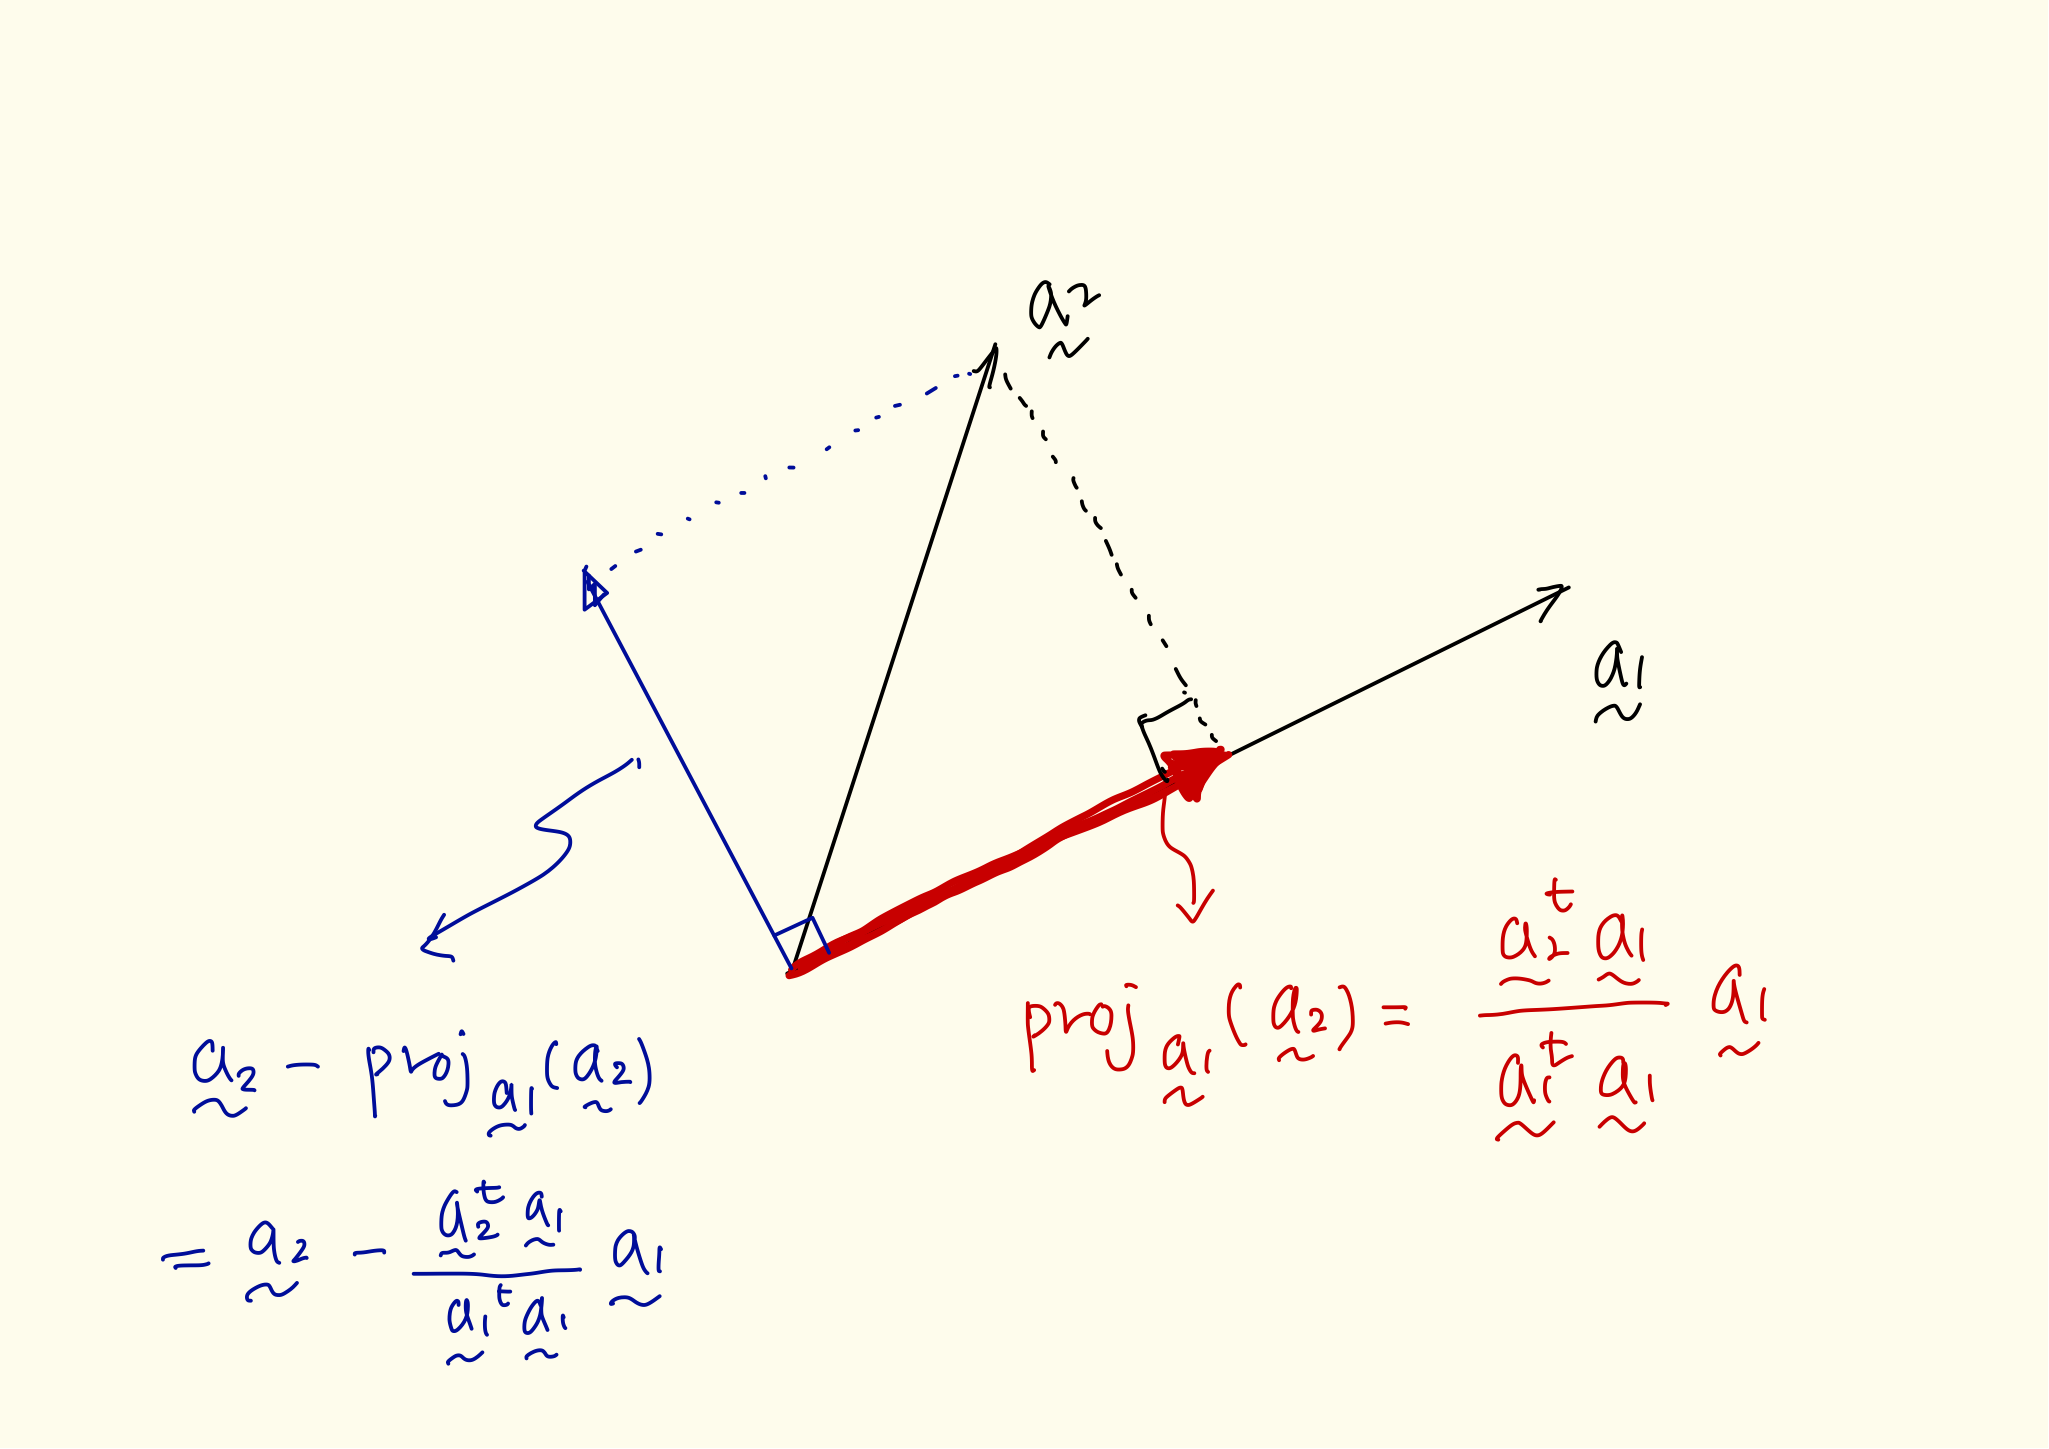
\includegraphics{proj1.png}
\caption{벡터의 사영}
\end{figure}

두 벡터 \(\bm a_1\)와 \(\tilde {\bm q}_2\)의 직교성은 다음과 같이 보일 수 있다.

\begin{align}
\bm a_1^t  \tilde {\bm q}_2 & =
 \bm a_1^t  \left ( \bm a_2 -  \frac{ \bm a_2^t \bm a_1} {\bm a_1^t \bm a_1} \bm a_1 \right ) \notag \\
 & = \bm a_1^t \bm a_2 - \frac{ \bm a_2^t \bm a_1} {\bm a_1^t \bm a_1}  \bm a_1^t \bm a_1 \notag \\
 & = \bm a_1^t \bm a_2 - \bm a_2^t \bm a_1 \notag \\
 & = 0 
 \label{eq:proofortho}
\end{align}

이제 두 벡터 \(\bm q_1\)과 \(\bm q_2\) 를 다음과 같이 정규직교벡터로 만들 수 있다.
\begin{align*}
\bm q_1 & =  \bm a_1 / \norm{\bm a_1 } \\
\bm q_2 & =  \tilde {\bm q}_2 / \norm{\tilde {\bm q}_2}
\end{align*}

\hypertarget{uxcd5cuxc18cuxc81cuxacf1uxbc95uxacfc-uxc0acuxc601}{%
\subsection{최소제곱법과 사영}\label{uxcd5cuxc18cuxc81cuxacf1uxbc95uxacfc-uxc0acuxc601}}

회귀계수벡터의 값을 구하는 최소제곱법의 기준을 다시 살펴보자.

\[   \min_{\bm \beta } \norm{\bm y -  \bm X \bm \beta }^2= \min_{\bm \beta } ( \bm y -  \bm X \bm \beta )^t( \bm y -  \bm X \bm \beta )  \]

위에서 \(\bm X \bm \beta\)는 행렬 \(\bm X\)의 열벡터 \(\bm x_0, \bm x_1, \dots, \bm x_p\) 로 이루어진 선형조합이다.

\[ \bm X \bm \beta = [\bm x_0~\bm x_1~ \cdots \bm x_p]\bm \beta
 = \beta_0 \bm x_0  + \beta_1 \bm x_1 + \cdots + \beta_p \bm x_p \]

따라서 최소제곱법으로 구한 회귀계수 벡터 \(\hat {\bm \beta}\)는 반응값 벡터 \(\bm y\) 와 \(\bm X {\bm \beta}\)의 거리가 최소가 되도록 만들어 준다.

\[ \hat {\bm \beta} = (\bm X^t \bm X)^{-1} \bm X^t \bm y, \quad 
 \min_{\bm \beta } \norm{\bm y -  \bm X \bm \beta }^2 = \norm{\bm y -  \bm X \hat {\bm \beta} }^2
 \]

따라서 예측값 벡터 \(\hat {\bm y}\) 는 행렬 \(\bm X\)의 열벡터로 생성한 열공간 방향으로 반응값 벡터 \(\bm y\)를 사영한 벡터이다.

\[ \hat {\bm y} = \bm X \hat {\bm \beta} = \bm  X(\bm X^t \bm X)^{-1} \bm X^t \bm y \]

위에서 행렬 \(\bm P = \bm X(\bm X^t \bm X)^{-1} \bm X^t\)를 열공간 \(C(\bm X)\)의 사영행렬(projection matrix)라고 부른다.

\begin{figure}
\centering
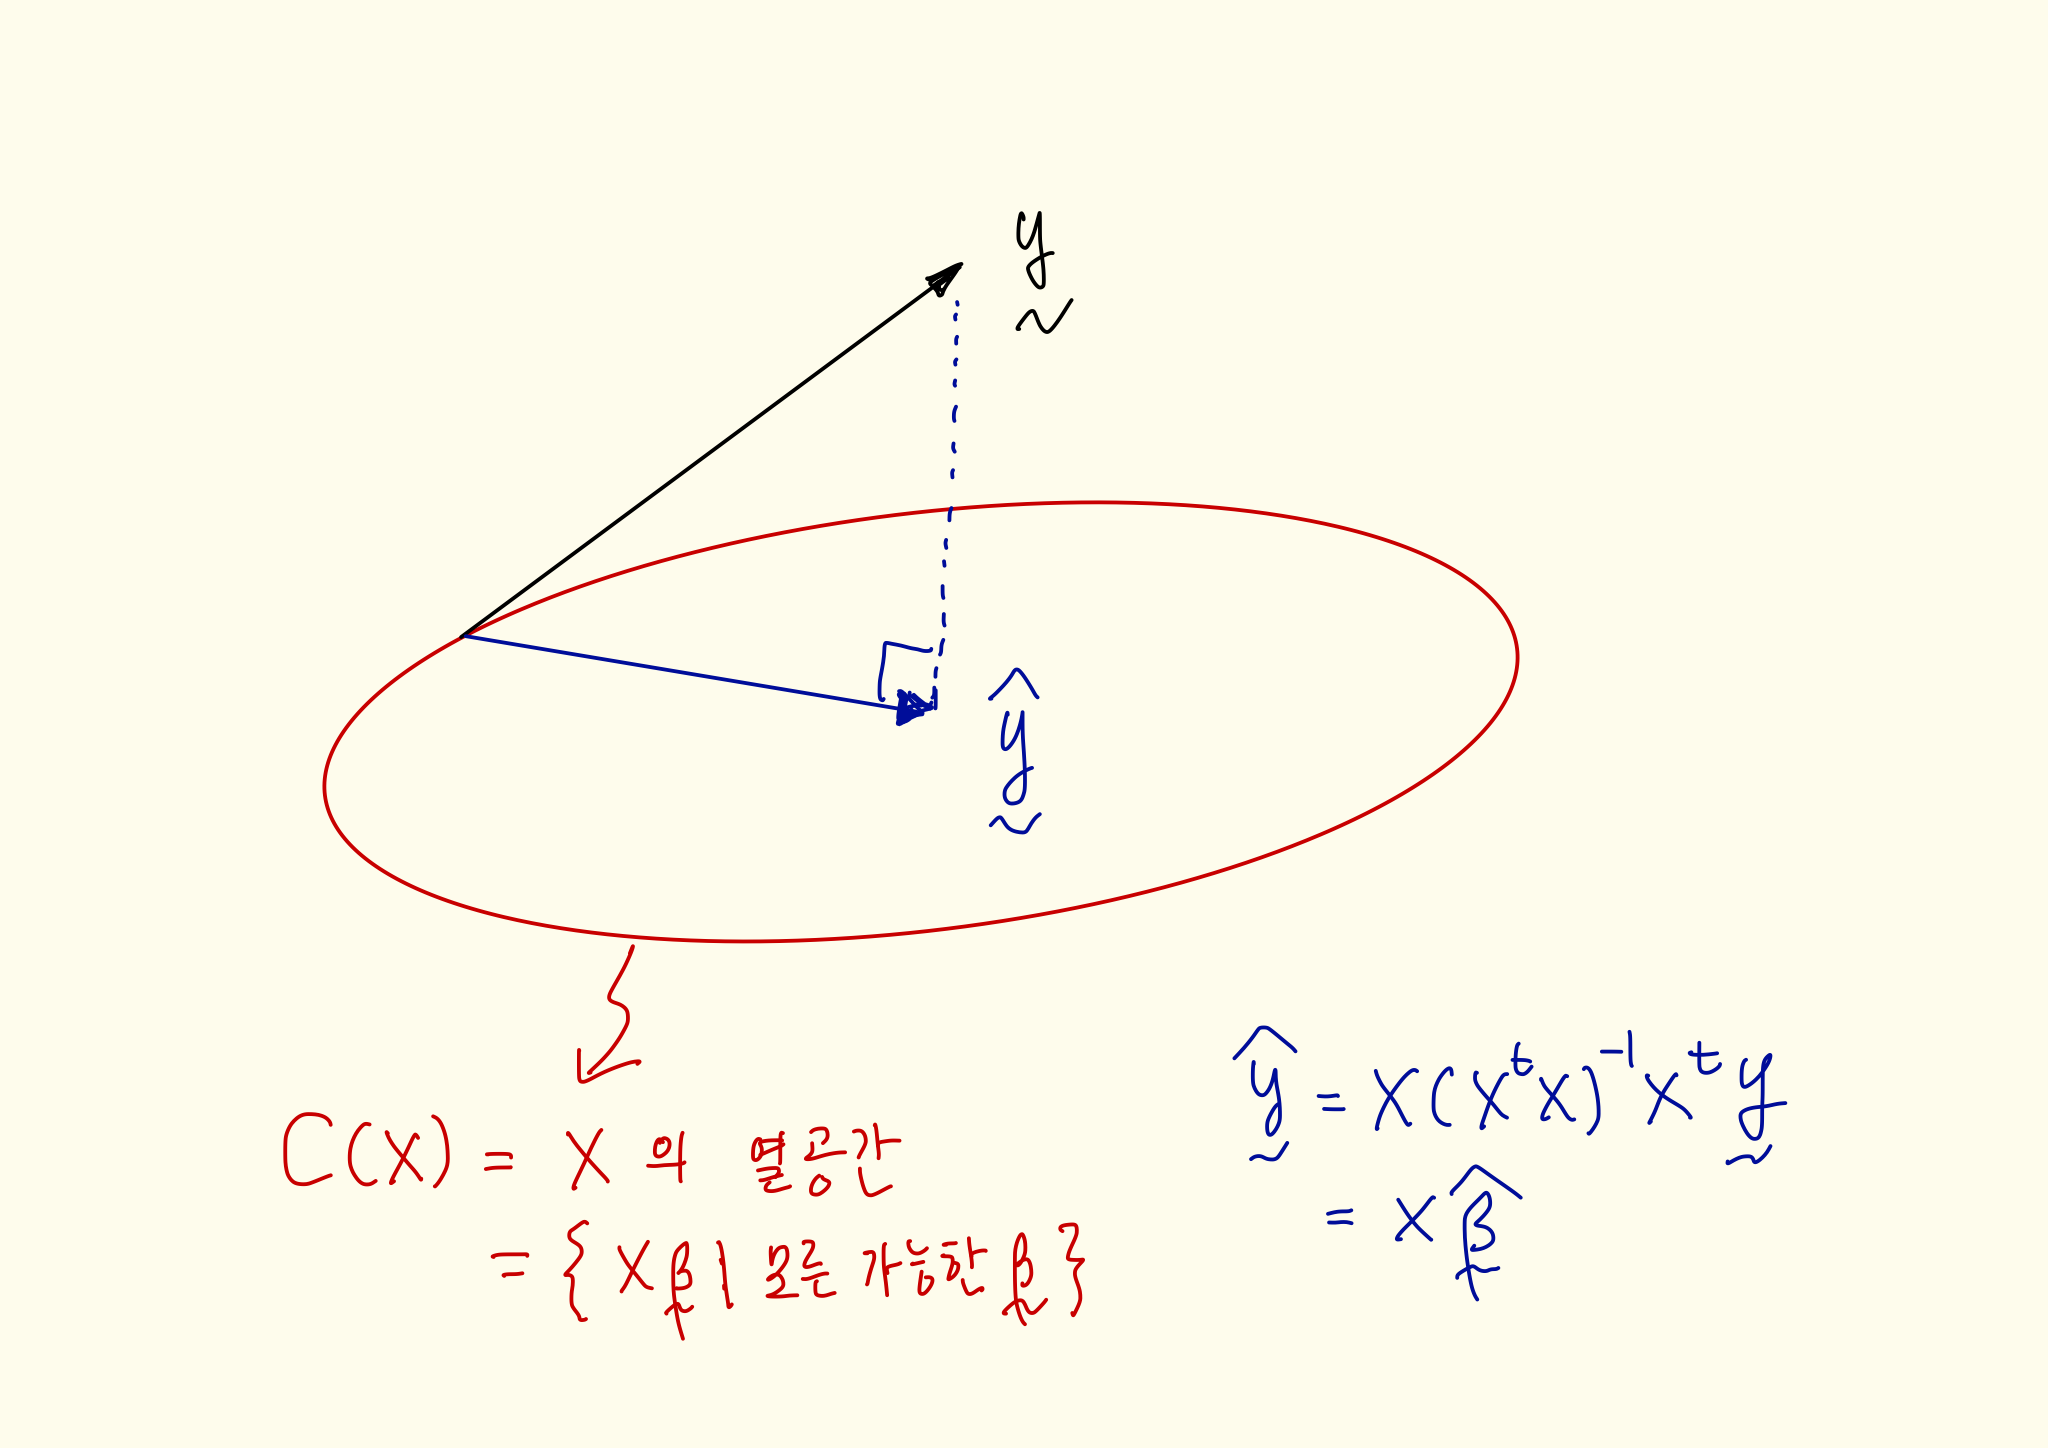
\includegraphics{proj2.png}
\caption{최소제곱법을 설명한 그림}
\end{figure}

\hypertarget{uxc6b0uxb4dcuxbca0uxb9ac-uxacf5uxc2ddwoodbury-formula}{%
\section{우드베리 공식(Woodbury formula)}\label{uxc6b0uxb4dcuxbca0uxb9ac-uxacf5uxc2ddwoodbury-formula}}

\[ (\bm A+\bm U\bm C\bm V)^{-1} = \bm A^{-1}-\bm A^{-1} \bm U (\bm C^{-1} + \bm V \bm A^{-1}\bm U)^{-1} \bm V \bm A^{-1} \]

\[ (\bm I+\bm U\bm C\bm V)^{-1} = \bm I - \bm U (\bm C^{-1} + \bm V \bm U)^{-1} \bm V \]

\[ (\bm A+\bm u\bm v^t)^{-1} = \bm A^{-1} - \frac{ \bm A^{-1} \bm u\bm v^t \bm A^{-1}}{1+\bm v^t \bm A^{-1}\bm u} \]

\[ (a \bm I_n + b \bm 1_n \bm 1_n^t)^{-1} = \frac{1}{a} \left [ \bm I_n - \frac{b}{a+nb} \bm 1 \bm 1^t \right ] \]

\hypertarget{mulivar}{%
\chapter{다변량 확률변수의 성질}\label{mulivar}}

\hypertarget{uxc77cuxbcc0uxb7c9uxbd84uxd3ec}{%
\section{일변량분포}\label{uxc77cuxbcc0uxb7c9uxbd84uxd3ec}}

일변량 확률변수 \(X\)가 확률밀도함수 \(f(x)\)를 가지는 분포를 따를때 기대값과 분산은 다음과 같이 정의된다.
\[ E(X) = \int x f(x)  dx = \mu, \quad V(X) = E[ X-E(X)]^2=\int (x-\mu)^2 f(x) dx =\sigma^2 \]

새로운 확률변수 \(Y\)가 확률변수 \(X\)의 선형변환으로 표시된다면 (\(a\)와 \(b\)는 실수)
\[ Y = aX+b\]
그 기대값(평균)과 분산은 다음과 같이 계산된다.
\begin{eqnarray*}
E(Y) &=& E(aX+b) \\
&=& \int (ax+b) f(x) dx \\
&=& a \int x f(x) dx + b \\
&=& a E(X) + b\\
&=& a \mu + b \\
V(Y) &=& Var(aX+b) \\
&=& E[aX+b -E(aX+b)]^2 \\
&=& E[a(X-\mu)]^2 \\
&=& a^2 E(X-\mu)^2\\
&=& a^2 \sigma^2
\end{eqnarray*}

\hypertarget{uxd655uxb960uxbca1uxd130uxc640-uxbd84uxd3ec}{%
\section{확률벡터와 분포}\label{uxd655uxb960uxbca1uxd130uxc640-uxbd84uxd3ec}}

확률벡터 \(\bm X\)가 \(p\) 차원의 다변량분포를 따른다고 하고 결합확률밀도함수 \(f(\bm x) =f(x_1,x_2,\dots,x_p)\)를
를 가진다고 하자.
\begin{equation*}
\bm X =
  \begin{pmatrix}
X_1 \\
X_2 \\
X_3 \\
..  \\
X_p
\end{pmatrix}
\end{equation*}

다변량 확률벡터의 기대값(평균벡터)과 공분산(행렬)은 다음과 같이 계산된다.
\begin{equation*}
\bm E(\bm X) =
  \begin{pmatrix}
E(X_1) \\
E(X_2) \\
E(X_3) \\
..  \\
E(X_p)
\end{pmatrix}
= 
  \begin{pmatrix}
\mu_1 \\
\mu_2 \\
..  \\
\mu_p
\end{pmatrix}
=\bm \mu
\end{equation*}

\begin{equation*}
V(\bm X) =Cov(\bm X) = E (\bm X-\bm \mu) (\bm X-\bm \mu)^t 
= 
  \begin{pmatrix}
\sigma_{11} & \sigma_{12} & \dots & \sigma_{1p} \\
\sigma_{12} & \sigma_{22} & \dots & \sigma_{2p} \\
& \dots & \dots & \\
\sigma_{1p} & \sigma_{2p} & \dots & \sigma_{pp} \\
\end{pmatrix}
= \bm \Sigma
\end{equation*}
여기서 \(\sigma_{ii}=V(X_i)\), \(\sigma_{ij} = Cov(X_i, X_j)=Cov(X_j, X_i)\)이다. 따라서 공분산 행렬
\(\bm \Sigma\)는 대칭행렬(symmetric matrix)이다. 다음 공식은 유용한 공식이다.
\[ \bm \Sigma = E (\bm X-\bm \mu) (\bm X-\bm \mu)^t  = E(\bm X \bm X^t)-\bm \mu \bm \mu^t \]

두 확률변수의 상관계수 \(\rho_{ij}\)는 다음과 같이 정의된다.
\[ \rho_{ij} = \frac{Cov(X_i, X_j)}{ \sqrt{V(X_i) V(X_j)}} = \frac{\sigma_{ij}}{\sqrt{\sigma_{ii}
  \sigma_{jj}}} \]

새로운 확률벡터 \(\bm Y\)가 확률벡터 \(\bm X\) 의 선형변환라고 하자.
\[ \bm Y = \bm A  \bm X + \bm b \]
단 여기서 \(\bm A = \{ a_{ij} \}\)는 \(p \times p\) 실수 행렬이고
\(\bm b =(b_1 b_2 \dots b_p)^t\)는 \(p \times 1\) 실수 벡터이다.

확률벡터 \(\bm Y\)의 기대값(평균벡터)과 공분산은 다음과 같이 계산된다.
\begin{eqnarray*}
E(\bm Y ) &=& E(\bm A \bm X+ \bm b) \\
&=& \bm A E(\bm X)+ \bm b \\
&=& \bm A \bm \mu+ \bm b \\
V(\bm Y) &=& Var(\bm A \bm X+ \bm b) \\
&=& E[\bm A \bm X+ \bm b -E(\bm A \bm X+ \bm b)] [\bm A \bm X+ \bm b -E(\bm A \bm X+ \bm b)]^t \\
&=& E[\bm A \bm X -  \bm A \bm \mu] [\bm A \bm X -  \bm A \bm \mu]^t \\
&=& E[\bm A (\bm X - \bm \mu)] [\bm A (\bm X - \bm \mu)]^t \\
&=& \bm A E [(\bm X - \bm \mu) (\bm X - \bm \mu)^t] \bm A^t \\
&=& \bm A \bm \Sigma \bm A^t
\end{eqnarray*}

만약 표본 \(\bm X_i, \bm X_2, \dots, \bm X_n\) 이 독립적으로 평균이 \(\bm \mu\) 이고 공분산이 \(\bm \Sigma\)
인 분포에서 추출되었다면 표본의 평균벡터 \(\bar {\bm X}\) 는 평균이 \(\bm \mu\) 이고 공분산이 \(\frac{1}{n}\bm \Sigma\)
인 분포를 따른다.
\begin{equation*}
\bar {\bm X} =
  \begin{pmatrix}
\sum_{i=1}^n X_{i1} / n  \\
\sum_{i=1}^n X_{i2} / n \\
\sum_{i=1}^n X_{i3} / n \\
..  \\
\sum_{i=1}^n X_{ip} / n 
\end{pmatrix}
\end{equation*}
여기서 \(X_{ij}\) 는 \(i\)번째 표본벡터 \(\bm X_i =(X_{i1} X_{i2} \dots X_{ip})^t\)의 \(j\)번째 확률변수이다.

\hypertarget{uxb2e4uxbcc0uxb7c9-uxc815uxaddcuxbd84uxd3ec}{%
\section{다변량 정규분포}\label{uxb2e4uxbcc0uxb7c9-uxc815uxaddcuxbd84uxd3ec}}

일변량 확률변수 \(X\)가 평균이 \(\mu\) 이고 분산이 \(\sigma^2\)인 정규분포를 따른다면 다음과 같이 나타내고 \[ X \sim N(\mu, \sigma^2 ) \]
확률밀도함수 \(f(x)\) 는 다음과 갇이 주어진다.
\[ f(x) = (2 \pi \sigma^2)^{-1/2} \exp \left ( - \frac{(x-\mu)^2}{2} \right ) \]

\(p\)-차원 확률벡터 \(\bm X\)가 평균이 \(\bm \mu\) 이고 공분산이 \(\bm \Sigma\)인
다변량 정규분포를 따른다면 다음과 같이 나타내고 \[ \bm X \sim N_p(\bm \mu, \bm \Sigma ) \]
확률밀도함수 \(f(\bm x)\) 는 다음과 갇이 주어진다.
\[ f(\bm x) = (2 \pi)^{-p/2} | \bm \Sigma|^{-1/2} 
   \exp \left ( - \frac{(\bm x-\bm \mu) \bm \Sigma^{-1}(\bm x-\bm \mu)^t}{2} \right ) \]

다변량 정규분포 \(N(\bm \mu, \bm \Sigma)\)를 따르는 확률벡터 \(\bm X\)를 다음과 같이 두 부분으로 나누면

\[ 
  \bm X = 
    \begin{bmatrix}
  \bm X_1 \\
  \bm X_2
  \end{bmatrix}, \quad
  \bm X_1 = 
    \begin{bmatrix}
  \bm X_{11} \\
  \bm X_{12} \\
  \bm \vdots \\
  \bm X_{1p}
  \end{bmatrix}, \quad 
  \bm X_2= 
    \begin{bmatrix}
  \bm X_{21} \\
  \bm X_{22} \\
  \bm \vdots \\
  \bm X_{2q}
  \end{bmatrix}
  \]

각각 다변량 정규분포를 따르고 다음과 같이 나타낼 수 있다.

\[ 
  \begin{bmatrix}
  E(\bm X_1) \\
  E(\bm X_2)
  \end{bmatrix}
  =
    \begin{bmatrix}
  \bm \mu_1 \\
  \bm \mu_2
  \end{bmatrix}
  , \quad 
  \begin{bmatrix}
  V(\bm X_1) & Cov(\bm X_1, X_2) \\
  Cov(\bm X_2 X_1) & V(\bm X_2)
  \end{bmatrix}
  =
    \begin{bmatrix}
  \bm \Sigma_{11} & \bm \Sigma_{12} \\
  \bm \Sigma^t_{12} & \bm \Sigma_{22}
  \end{bmatrix}
  \]

\[  \bm X =
    \begin{bmatrix}
  \bm X_1 \\
  \bm X_2
  \end{bmatrix}
  \sim
  N_{p+q} \left (
    \begin{bmatrix}
    \bm \mu_1 \\
    \bm \mu_2
    \end{bmatrix}
    ,\begin{bmatrix}
    \bm \Sigma_{11} & \Sigma_{12} \\
    \bm \Sigma^t_{12} & \Sigma_{22}
    \end{bmatrix}
    \right )
  \]

확률벡터 \(\bm X_2 = \bm x_2\)가 주어진 경우 \(\bm X_1\)의 조건부 분포는 \(p\)-차원 다변량 정규분포를 따르고 평균과 공분산은 다음과 같다.

\[ 
  E(\bm X_1 | \bm X_2 = \bm x_2 ) = \bm \mu_1 + \bm \Sigma_{12} \bm \Sigma^{-1}_{22} (\bm \mu_2 - \bm x_2), \quad
  V(\bm X_1 | \bm X_2 = \bm x_2 )  = \bm \Sigma_{11} -\bm \Sigma_{12} \bm \Sigma^{-1}_{22} \bm \Sigma^t_{12}
  \]

예를 들어 \(2\)-차원 확률벡터 \(\bm X=(X_1, X_2)^t\)가 평균이 \(\bm \mu=(\mu_1,\mu_2)^t\) 이고
공분산 \(\bm \Sigma\)가 다음과 같이 주어진
\begin{equation*}
\bm \Sigma =
  \begin{pmatrix}
\sigma_{11} & \sigma_{12} \\
\sigma_{12} & \sigma_{22}
\end{pmatrix}
\end{equation*}
이변량 정규분포를 따른다면 확률밀도함수 \(f(\bm x)\)에서 \(\exp\)함수의 인자는 다음과 같이 주어진다.
\begin{eqnarray*}
&(\bm x-\bm \mu) \bm \Sigma^{-1}(\bm x-\bm \mu)^t
= \\
&-\frac{1}{2 (1-\rho^2)} 
\left [ 
  \left ( \frac{(x_1-\mu_1)^2}{\sigma_{11}} \right )
  +\left ( \frac{(x_2-\mu_2)^2}{\sigma_{22}} \right )
  -2 \rho \left ( \frac{(x_1-\mu_1)}{\sqrt{\sigma_{11}}} \right )
  \left ( \frac{(x_2-\mu_2)}{\sqrt{\sigma_{22}}} \right )
  \right ]
\end{eqnarray*}
그리고 \(p=2\)인 경우 확률밀도함수의 상수부분은 다음과 같이 주어진다.
\[ (2 \pi)^{-p/2} | \bm \Sigma|^{-1/2} = \frac{1}{ 2 \pi \sqrt{\sigma_{11} \sigma_{22} (1-\rho^2)}} \]
여기서 \(\rho = \sigma_{12} / \sqrt{\sigma_{11} \sigma_{22}}\)

만약 \(X_2 = x_2\)가 주어졌을 때 \(X_1\)의 조건부 분포는 정규분포이고 평균과 분산은 다음과 같이 주어진다.

\[ 
  E( X_1 |  X_2 =  x_2 ) =  \mu_1 +  \frac{\sigma_{12}}{\sigma_{22}} ( \mu_2 -  x_2)  = \mu_1 +  \rho \frac{\sqrt{\sigma_{11}}}{\sqrt{\sigma_{22}}} ( \mu_2 -  x_2) \]

\[
  V( X_1 |  X_2 =  x_2 )  =  \sigma_{11} - \frac{\sigma^2_{12}}{\sigma_{22}}  = \sigma_{11}(1-\rho^2)
  \]

다변량 정규분포에서 공분산이 0인 두 확률 변수는 독립이다.
\[ \sigma_{ij} = 0 \leftrightarrow X_i \text{ and } X_j \text{ are independent} \]

\hypertarget{uxd45cuxc900uxc815uxaddcuxbd84uxd3ecuxb85cuxc758-uxbcc0uxd658}{%
\section{표준정규분포로의 변환}\label{uxd45cuxc900uxc815uxaddcuxbd84uxd3ecuxb85cuxc758-uxbcc0uxd658}}

일변량 확률변수 \(X\)가 평균이 \(\mu\) 이고 분산이 \(\sigma^2\)인 경우 다음과 같은 선형변환을 고려하면.
\[ Z = \frac{X - \mu}{\sigma} = (\sigma^2)^{-1/2} (X-\mu) \]
확률변수 \(Z\) 는 평균이 \(0\) 이고 분산이 \(1\)인 분포를 따른다.

\(p\)차원 확률벡터 \(\bm X\) 가 평균이 \(\bm \mu\) 이고 공분산이 \(\bm \Sigma\)인 분포를 가진다고 가정하자.
공분산 행렬 \(\bm \Sigma\)는 양정치 행렬(positive definite matrix)이며 다음과 같은 행렬의 분해가 가능하다.
\[ \Sigma = \bm C \bm C^t \]
여기서 \(\bm C\) 는 정칙행렬이며 역행렬 \(\bm C^{-1}\)가 존재한다.
위와 같은 행렬의 분해는 스펙트럴 분해(spectral decomposition)을 이용하여 구할 수 있다. 공분산 행렬 \(\bm \Sigma\)는 양정치 행렬이므로 고유치(eigen value) \((\lambda_1, \lambda_2,\dots, \lambda_p)\)가 모두 양수이고 정규직교 고유벡터(orthonormal eigen vector)의 행렬 \(\bm P\)을 이용하여 다음과 같은 분해가 가능하다.
\[ \Sigma = \bm P \bm \Lambda \bm P^t = \bm P \bm \Lambda^{1/2} \Lambda^{1/2} \bm P^t \]
여기서 \(\bm \Lambda\)는 고유치 \((\lambda_1, \lambda_2,\dots, \lambda_p)\)를 대각원소로 가지는
대각행렬이며 \(\bm \Lambda^{1/2}\)는 고유치의 제곱근을 대각원소로 가지는
대각행렬이다. 따라서 \(\bm C = \bm P \bm \Lambda^{1/2}\)로 하면 위와 같은 행렬의 분해가 가능하다.
정규직교 고유벡터(orthonormal eigen vector)의 행렬 \(\bm P\)는 직교행렬이므로
\[ \bm C^{-1} =  (\bm P \bm \Lambda^{1/2})^{-1} = \bm \Lambda^{-1/2} \bm P^t \]

\(p\)차원 확률벡터 \(\bm X\)의 다음과 같은 선형변환을 고려하면.
\[ \bm Z = \bm C^{-1} ( \bm X- \bm \mu) = \bm \Lambda^{-1/2} \bm P^t ( \bm X- \bm \mu)  \]
확률벡터 \(\bm Z\) 는 평균이 \(\bm 0\) 이고 공분산이 \(\bm I\)인 분포를 따른다 (why?).

확률벡터 \(\bm X\)가 정규분포를 따른다면 선형변환한 확률벡터 \(\bm Z\)도 정규분포를 따른다.

\hypertarget{uxc608uxc81c-1}{%
\section{예제}\label{uxc608uxc81c-1}}

예를 들어 이변량확률벡터 \(\bm X\)가 다음과 같은 평균벡터와 공분산을 가진 정규분포를 따른다고 하자
\begin{equation*}
\bm \mu =
  \begin{pmatrix}
1\\
2
\end{pmatrix}
\quad
\bm \Sigma =
  \begin{pmatrix}
2 & 1\\
1 & 2
\end{pmatrix}
\end{equation*}

공분산행렬 \(\bm \sigma\)의 고유치는 \(|\bm \sigma -\lambda \bm I|=0\)의 방정식을 풀어 구할 수 있다.
\begin{equation*}
|\bm \sigma -\lambda \bm I|  =
  \begin{pmatrix}
2-\lambda & 1\\
1 & 2-\lambda
\end{pmatrix}
= \lambda^2 -4 \lambda +3=0
\end{equation*}
방정식을 풀면 고유치는 \((\lambda_1, \lambda_2) = (3,1)\)이다. 각 고유치에 대한 고유벡터 \(\bm p=(p_1, p_2)^t\)는 \(\bm \Sigma \bm p = \lambda \bm p\) 으로 구할 수 있다. 각 고유치에 대하여 방정식을 구하면 다음 두 개의 방정식을 얻을 수 있다.
\begin{equation*}
p_1 - p_2 = 1 \text{ and } p_1 + p_2 = 0
\end{equation*}
정규직교 벡터의 조건을 만족 시키기 위해서 \(p^2_1 + p^2_2=1\)의 조건을 적용하면 다음과 같은
정규직교 고유행렬을 얻을 수 있다.
\begin{equation*}
\bm P =
  \begin{pmatrix}
\frac{1}{\sqrt{2}} & -\frac{1}{\sqrt{2}}\\
\frac{1}{\sqrt{2}} & \frac{1}{\sqrt{2}}
\end{pmatrix}
\end{equation*}
또한
\begin{equation*}
\bm \Lambda =
  \begin{pmatrix}
3 & 0\\
0 & 1
\end{pmatrix}
\quad
\bm \Lambda^{1/2} =
  \begin{pmatrix}
\sqrt{3} & 0\\
0 & 1
\end{pmatrix}
\end{equation*}
따라서 \(C^{-1} = \Lambda^{-1/2} \bm P^t\) 이며
\begin{equation*}
\bm C^{-1} =
  \bm \Lambda^{-1/2} \bm P^t =
  \begin{pmatrix}
\frac{1}{\sqrt{3}} & 0\\
0 & 1
\end{pmatrix}
\begin{pmatrix}
\frac{1}{\sqrt{2}} & \frac{1}{\sqrt{2}}\\
-\frac{1}{\sqrt{2}} & \frac{1}{\sqrt{2}}
\end{pmatrix}
=
  \begin{pmatrix}
\frac{1}{\sqrt{6}} & \frac{1}{\sqrt{6}}\\
-\frac{1}{\sqrt{2}} & \frac{1}{\sqrt{2}}
\end{pmatrix}
\end{equation*}

위의 계산을 R 프로그램으로 다음과 같이 구현할 수 있다.

\begin{Shaded}
\begin{Highlighting}[]
\NormalTok{mu }\OtherTok{\textless{}{-}} \FunctionTok{c}\NormalTok{(}\DecValTok{1}\NormalTok{,}\DecValTok{2}\NormalTok{)}
\NormalTok{S }\OtherTok{\textless{}{-}} \FunctionTok{matrix}\NormalTok{(}\FunctionTok{c}\NormalTok{(}\DecValTok{2}\NormalTok{,}\DecValTok{1}\NormalTok{,}\DecValTok{1}\NormalTok{,}\DecValTok{2}\NormalTok{),}\DecValTok{2}\NormalTok{,}\DecValTok{2}\NormalTok{)}
\NormalTok{res}\OtherTok{\textless{}{-}} \FunctionTok{eigen}\NormalTok{(S)}
\NormalTok{res}
\end{Highlighting}
\end{Shaded}

\begin{verbatim}
## eigen() decomposition
## $values
## [1] 3 1
## 
## $vectors
##           [,1]       [,2]
## [1,] 0.7071068 -0.7071068
## [2,] 0.7071068  0.7071068
\end{verbatim}

\begin{Shaded}
\begin{Highlighting}[]
\NormalTok{L }\OtherTok{\textless{}{-}}\NormalTok{ res}\SpecialCharTok{$}\NormalTok{values}
\NormalTok{P }\OtherTok{\textless{}{-}}\NormalTok{ res}\SpecialCharTok{$}\NormalTok{vectors}
\NormalTok{Lsqrt }\OtherTok{\textless{}{-}} \FunctionTok{diag}\NormalTok{(}\FunctionTok{sqrt}\NormalTok{(L))}
\NormalTok{C }\OtherTok{\textless{}{-}}\NormalTok{ P }\SpecialCharTok{\%*\%}\NormalTok{ Lsqrt}
\NormalTok{C}
\end{Highlighting}
\end{Shaded}

\begin{verbatim}
##          [,1]       [,2]
## [1,] 1.224745 -0.7071068
## [2,] 1.224745  0.7071068
\end{verbatim}

\begin{Shaded}
\begin{Highlighting}[]
\NormalTok{Cinv }\OtherTok{\textless{}{-}} \FunctionTok{solve}\NormalTok{(C)}
\NormalTok{Cinv }
\end{Highlighting}
\end{Shaded}

\begin{verbatim}
##            [,1]      [,2]
## [1,]  0.4082483 0.4082483
## [2,] -0.7071068 0.7071068
\end{verbatim}

\begin{Shaded}
\begin{Highlighting}[]
\NormalTok{Cinv }\SpecialCharTok{\%*\%}\NormalTok{ S }\SpecialCharTok{\%*\%} \FunctionTok{t}\NormalTok{(Cinv)}
\end{Highlighting}
\end{Shaded}

\begin{verbatim}
##      [,1] [,2]
## [1,]    1    0
## [2,]    0    1
\end{verbatim}

\hypertarget{quadratic}{%
\chapter{이차형식의 분포}\label{quadratic}}

\hypertarget{uxbe44uxc911uxc2ec-chi2-uxbd84uxd3ec}{%
\section{\texorpdfstring{비중심 \(\chi^2\) 분포}{비중심 \textbackslash chi\^{}2 분포}}\label{uxbe44uxc911uxc2ec-chi2-uxbd84uxd3ec}}

만약 확률변수 \(x\)가 \(N(\mu, 1)\)을 따른다면 \(v=x^2\)은 비중심 \(\chi^2\) 분포, \(\chi^2_1(\lambda^2)\) 를 따른다. 여기서 비중심 \(\chi^2\) 분포의 자유도는 1이고 비중심모수 \(\lambda^2 = \mu^2\)으로 주어진다.

만약 확률변수 \(x\)가 \(N(0, 1)\)을 따른다면 \(v=x^2\)은 중심 \(\chi^2\) 분포, \(\chi^2_1\) 를 따르며 이때는 비중심모수가 \(\lambda^2=0\)이다.

이제 \(n\)개의 서로 독립인 확률 변수 \(x_1,x_2,\cdots,x_n\)이 각각 \(N(\mu_i, 1)\)을 따른다면 \(v=x_1^2+\dots+x_n^2\)은 자유도가 \(n\)이고 비중심 모수가 \(\lambda^2 = \sum_{i=1}^n \mu_i^2\)인 비중심 \(\chi^2\) 분포, \(\chi^2_n(\lambda^2)\) 를 따른다. 비중심모수가 0 이면 자유도가 \(n\)인 (중심) 카이제곱 분포를 따른다.

\hypertarget{uxc774uxcc28uxd615uxc2dduxc758-uxbd84uxd3ec}{%
\section{이차형식의 분포}\label{uxc774uxcc28uxd615uxc2dduxc758-uxbd84uxd3ec}}

\(n\)개의 서로 독립인 확률 변수 \(x_1,x_2,\cdots,x_n\)이 각각 \(N(\mu_i, \sigma^2)\)를 따른다면
\(n\)-차원의 확률벡터 \(\bm x\)는 다음과 같은 다변량 정규분포를 따른다고 할 수 있다.

\[ \bm x \sim N(\bm \mu, \sigma^2 \bm I) \]

위에서 \(\bm \mu^t =(\mu_1, \mu_2, \dots, \mu_n)\)

이제 이차형식의 분포에 대하여 논의하자.

\begin{theorem}[Distribution of quadratic form]
\protect\hypertarget{thm:unnamed-chunk-29}{}{\label{thm:unnamed-chunk-29} \iffalse (Distribution of quadratic form) \fi{} }\(n\)-차원의 확률벡터 \(\bm x\)가 \(N(\bm \mu, \sigma^2 \bm I)\)를 따른 다면 이차형식 \(Q=\bm x^t \bm A \bm x\)의 분포는 다음과 같다.

\begin{equation}
V = \frac{Q}{\sigma^2} = \frac {\bm x^t \bm A \bm x}{\sigma^2} ~~ \equiv_d ~~ \sum_{i=1}^n \lambda_i \frac{u^2_i}{\sigma^2}
\label{eq:quaddist1}
\end{equation}

위에서 행렬 \(\bm A\)의 스펙트럴 분해는 \(\bm A = \bm P \bm \Lambda \bm P^t\)이며 \(\lambda_i\)는 행렬 \(\bm A\)의 고유치, 즉 행렬 \(\bm \Lambda\)의 대각원소이다. 또한 확률변수 \(u_i\)들은 서로 독립이며 정규분포 \(N(\eta_i, \sigma^2)\)를 따른다. 여기서 \(\eta_1, \eta_2,\dots, \eta_n\)는 다음과 같이 정의된다.
\[ 
\bm \eta =
\begin{bmatrix}
\eta_1 \\
\eta_2 \\
\vdots \\
\eta_n 
\end{bmatrix} =
  \bm P^t \bm \mu
\]
즉, 식 \eqref{eq:quaddist1}에서 \(u_1^2/\sigma^2, u_2^2/\sigma^2, \dots, u_n^2/\sigma^2\)는 서로 독립이며 각각 자유도가 1 이고 비중심 모수가 \(\eta_1^2/\sigma^2, \eta_2^2/\sigma^2, \dots, \eta_n^2/\sigma^2\)인 비중심 \(\chi^2\)-분포를 따른다. \(\blacksquare\)
\end{theorem}

위의 정리의 증명은 다음과 같은 변환를 이용한다.

\[ 
\frac{\bm x^t \bm A \bm x}{\sigma^2}  = \frac{\bm x^t \bm P \bm \Lambda \bm P^t \bm x}{\sigma^2}   = \frac{\bm u^t \bm \Lambda  \bm u}{\sigma^2} = \sum_{i=1}^n \lambda_i \left [ \frac{u_i}{\sigma} \right ]^2 
\]

여기서 확률벡터 \(\bm u = \bm P^t \bm x\) 는 \(N(\bm P^t \bm \mu, \sigma^2 \bm P^t \bm P ) = N(\bm \eta, \sigma^2 \bm I)\)를 따른다.

식 \eqref{eq:quaddist1}에서 나타난 이차형식의 분포는 비중심 카이제곱 분포를 따르는 \textbf{서로 독립인인 확률 변수들의 가중 평균}과 같다는 것이다. 이는 이차형식의 분포가 비중심 카이제곱 분포를 따른다는 것이 아님을 주의해야 한다. 그러면 어느 경우에 이차형식의 분포가 비중심 카이제곱 분포를 따르는가 생각해 보자. 가장 쉽게 생각할 수 있는 경우가 식 \eqref{eq:quaddist1}에서 \(\lambda_i\)들의 값들이 0 또는 1인 경우이다. 이러한 경우는 행렬 \(\bm A\)가 멱등행렬인 경우이다. 실제로 다음 정리는 이차형식의 분포가 비중심 카이제곱 분포를 따르는 필요충분 조건이 행렬 \(\bm A\)가 멱등행렬이라는 것을 말해준다.

\begin{corollary}
\protect\hypertarget{cor:unnamed-chunk-30}{}{\label{cor:unnamed-chunk-30} }\(n\)-차원의 확률벡터 \(\bm x\)가 \(N(\bm \mu, \sigma^2 \bm I)\)를 따른다면 이차형식 \(\bm x^t \bm A \bm x /\sigma^2\)의 분포가 자유도가 \(r\)이며 다음과 같은 비중심 모수 \(\lambda^2\)을 가지는 비중심 카이제곱 분포를 따르는 필요충분 조건은 \(\bm A\)가 멱등행렬이고 계수가 \(rank(\bm A =r)\)인 경우이다.

\[ \lambda^2 = \frac{\bm \mu^t \bm A \bm \mu}{\sigma^2} \]

더 나아가 \(\bm A \bm \mu=\bm 0\)인 경우에는 자유도가 \(r\)인 (중심)카이제곱 분포를 따른다. \(\blacksquare\)
\end{corollary}

참고로 이차형식의 기대값과 분산은 다음과 같이 주어진다.

\begin{equation}
E(\bm x^t \bm A \bm x) = \sigma^2 tr(\bm A) + \bm \mu^t \bm A \bm \mu, \quad
V(\bm x^t \bm A \bm x) = 2 \sigma^4 tr(\bm A^2) +4 \sigma^2 \bm \mu^t \bm A^2 \bm \mu
\label{eq:quadmean}
\end{equation}

\hypertarget{uxc774uxcc28uxd615uxc2dduxc758-uxb3c5uxb9bd}{%
\section{이차형식의 독립}\label{uxc774uxcc28uxd615uxc2dduxc758-uxb3c5uxb9bd}}

두 개의 이차형식이 독립일 조건은 다음 정리와 같다.

\begin{theorem}[independence of quadratic forms]
\protect\hypertarget{thm:unnamed-chunk-31}{}{\label{thm:unnamed-chunk-31} \iffalse (independence of quadratic forms) \fi{} }\(n\)-차원의 확률벡터 \(\bm x\)가 \(N(\bm \mu, \sigma^2 \bm I)\)를 따른다고 하자. 두 이차형식 \(Q_1=\bm x^t \bm A \bm x\) 과 \(Q_2=\bm x^t \bm B \bm x\) 가 서로 독립일 필요충분 조건은
\(\bm A \bm B= \bm 0\)이다. \(\blacksquare\)
\end{theorem}

만약 3개의 이차형식 \(Q, Q_1, Q_2\)가 있어서 다음과 같은 관계가 있다고 하자.

\[ Q =\bm x^t \bm A \bm x =  Q_1 + Q_2 =\bm x^t \bm A_1 \bm x + \bm x^t \bm A_2 \bm x \]

이러한 경우 두 이차형식 \(Q\)과 \(Q_1\)이 각각 카이제곱 분포를 따를 때 \(Q_2 = Q-Q_1\)이 카이제곱 분포를 따르는 조건이 중요하다. 다음 정리는 그 조건을 행렬 \(\bm A_2\)가 양반정치인 경우라는 것을 말해준다.

\begin{theorem}
\protect\hypertarget{thm:unnamed-chunk-32}{}{\label{thm:unnamed-chunk-32} }\(n\)-차원의 확률벡터 \(\bm x\)가 \(N(\bm \mu, \sigma^2 \bm I)\)를 따른다고 하자. 세 개의 이차형식 \(Q=\bm x^t \bm A \bm x\), \(Q_1=\bm x^t \bm A_1 \bm x\), \(Q_2=\bm x^t \bm A_2 \bm x\) 가 있다고 하고 \(Q=Q_1+Q_2\)인 관계를 가진다고 가정하자.

만약 \(Q/\sigma^2\)이 \(\chi^2_r(\lambda^2)\)을 따르고 \(Q_1/\sigma^2\)이 \(\chi^2_{r_1}(\lambda_1^2)\)을 따르며 행렬 \(\bm A_2\)가 양반정치 행렬이면 다음을 만족한다.

두 이차형식 \(Q_1\)과 \(Q_2\)는 서로 독립이다. 또한 이차형식 \(Q_2\)는 자유도가 \(r_2 = r-r_1\)이고 비중심 모수가 \(\lambda_2^2 = \lambda^2 -\lambda_1^2\)인 비중신ㅁ 카이제곱분포를 따른다. \(\blacksquare\)
\end{theorem}

\hypertarget{uxcf54uxd06cuxb780uxc758-uxc815uxb9ac}{%
\section{코크란의 정리}\label{uxcf54uxd06cuxb780uxc758-uxc815uxb9ac}}

선형모형에서 자주 등장하는 제곱합들의 분해, 즉 이차형식의 분해를 생각할 때 각 제곱합들의 분포를 아는 것이 매우 중요하다. 다음에 제시된 코크란의 정리(Chchran's Theorem)는 총 제곱합을 분해했을 때 각 제곱합의 분포가 카이제곱 분포를 따를 조건을 말해준다.

\begin{theorem}[COCHRAN'S THEOREM]
\protect\hypertarget{thm:unnamed-chunk-33}{}{\label{thm:unnamed-chunk-33} \iffalse (COCHRAN'S THEOREM) \fi{} }\(n\)-차원의 확률벡터 \(\bm x\)가 \(N(\bm \mu, \sigma^2 \bm I)\)를 따른다고 하자. \(k\) 개의 이차형식 \(Q_j=\bm x^t \bm A_j \bm x\), \(j=1,2,\dots,k\)를 생각하고 다음과 같은 관계를 가진다고 하자.

\[ \bm x^t \bm x = \sum_{i=1}^n x_i^2 = \sum_{j=1}^k Q_j \]

즉, \(\sum_{j=1}^k \bm A_j = \bm I\)이다. 또한 \(r_j =rank(\bm A_j)\) 이고 \(\lambda_j^2 = \bm \mu^t \bm A_{j} \bm \mu\) 라고 하자.

\(k\)개의 이차형식 \(Q_1, Q_2, \dots , Q_k\) 들이 모두 독립이고 각 이차형식 \(Q_j/\sigma^2\)가 비중심 카이제곱 분포 \(\chi^2_{r_{j}}(\lambda_j^2)\)를 따를 필요중분 조건은 다음과 같다.

\begin{equation}
r_1 + r_2 + \dots + r_{k} = n
\label{eq:cochran}
\end{equation}

\(\blacksquare\)
\end{theorem}

이제 제곱합의 분포들에 대하여 지금까지 학습한 내용을 정리해보자. 만약 \(n\)-차원의 확률벡터 \(\bm x\)가 \(N(\bm \mu, \sigma^2 \bm I)\)를 따른다고 하고 위의 코크란의 정리와 같이 제곱합의 분해를 고려하자. 다음에 제시된 모든 문장은 서로 동치(equivalent)이다.

\begin{enumerate}
\def\labelenumi{\arabic{enumi}.}
\tightlist
\item
  이차형식 \(Q_1, Q_2, \dots , Q_k\) 들이 모두 독립이다.
\item
  모든 \(j=1,2,\dots,k\)에 대하여 이차형식 \(Q_j/\sigma^2\)가 비중심 카이제곱 분포 \(\chi^2_{r_{j}}(\lambda_j^2)\)를 따른다.
\item
  \(\bm A_1, \bm A_2, \dots, \bm A_k\)가 모두 멱등행렬이다.
\item
  모든 \(j \ne k\)에 대하여 \(\bm A_j \bm A_k = \bm 0\) 이다.
\item
  \(r_1 + r_2 + \dots + r_{k} = n\)
\end{enumerate}

\hypertarget{vectordiff}{%
\chapter{벡터미분}\label{vectordiff}}

\hypertarget{uxc2a4uxce7cuxb77cuxbbf8uxbd84}{%
\section{스칼라미분}\label{uxc2a4uxce7cuxb77cuxbbf8uxbd84}}

벡터미분(Vector diffrential) 또는 행렬미분(Matrix differential)은 벡터와 행렬의 미분식에 대한 표기법을
정의하는 방법이다. 보통 스칼라(scalar)에 대한 미분은 일분수 함수 \(f: \Re^1 \rightarrow \Re^1\)또는 다변수 함수(function of several variables) \(f: \Re^p \rightarrow \Re^1\)에서 쉽게 정의된다. 만약 \(y = f(x)\) 또는 \(y=f(\bm x)\)라고 하면 다음과 같이 미분이 주어진다.

\[ \pardiff{y}{x}= \pardiff{f(x)}{x} = f'(x)  \]

\[ \pardiff{y}{\bm x} =\pardiff{f(\bm x)}{\bm x} =  \left (\pardiff{f(\bm x)}{x_1},~\pardiff{f(\bm x)}{x_2},~\cdots, \pardiff{f(\bm x)}{x_p} \right )  = \nabla  f(x)\]
함수가 다변수함수일 경우 함수의 값을 각 축의 변수로 미분한 것(partial derivative)을 벡터로 표시하는 것을 gradient 라고 한다.

\hypertarget{uxbca1uxd130uxbbf8uxbd84uxc758-uxd45cuxae30-uxbc29uxbc95}{%
\section{벡터미분의 표기 방법}\label{uxbca1uxd130uxbbf8uxbd84uxc758-uxd45cuxae30-uxbc29uxbc95}}

이제 다변량함수(multivariate function), \(f: \Re^p \rightarrow \Re^q\)에 대한 미분을 생각해보자. 앞 절에서
본것과 같이 스칼라 함수를 여러 변수로 미분하여 partial derivative를 구한 뒤 gradient를 만드는 경우 열벡터와 행벡터 중 하나를 선택해야 한다. 이러한 선택은 절대적인 것이 아니며 각 분야의 특성과 편의에 따라 다르게 선택 될 수 있다.

이제 간단한 예제를 고려해 보자. 두 열벡터 \(\bm x=(x_1,x_2)^t \in \Re_2\), \(\bm y=(y_1,y_2,y_3)^t \in \Re^3\)를 고려하고 다음과 같은 함수로 두 벡터의 관계가 정의된다고 하자.
\[ y_1 = x_1^2 + x_2, \quad y_2= \exp (x_1) + 3 x_2, \quad y_3 = \sin(x_1) + x_2^3 \]

일단 각각의 partial derivative \(\pardiffl{y_i}{x_j}\)를 구해야 하며 이는 scalar 미분으로 쉽게 구해진다.
\begin{align*}
\pardiff{  y_1}{ x_1} & = 2x_1, & \quad \pardiff{  y_2}{ x_1} & = \exp(x_1), & \quad
\pardiff{  y_3}{ x_1} & = \cos(x_1) \\
\pardiff{  y_1}{ x_2} & = 1,    & \quad \pardiff{  y_2}{ x_1} & = 3,         & \quad
\pardiff{  y_3}{ x_1} & = 3 x_2^2 \\
\end{align*}

통계학에서는 벡터 \(\bm y\)를 벡터 \(\bm x\)로 미분하려면 다음과 같이 분모 표기법 (Denominator layout)을 사용하여 표기한다.

\begin{equation*}
\pardiff{ \bm y}{\bm x}  \equiv \pardiff{ \bm y^t}{\bm x}
\underset{def}{\equiv} \begin{bmatrix}
\pardiff{  y_1}{ x_1} &  \pardiff{  y_2}{ x_1} &  \pardiff{  y_3}{ x_1}  \\
\pardiff{  y_1}{ x_2} &  \pardiff{  y_2}{ x_2} &  \pardiff{  y_3}{ x_2}  \\
\end{bmatrix}
=  \begin{bmatrix}
2x_1 &  \exp(x_1) & \cos(x_1)  \\
1 &  3  &  3x_2^2
\end{bmatrix}
\end{equation*}

즉 분모표기법은 분모를 열벡터로, 분자를 행벡터로 보고 각각 위치에 있는 변수들에 대하여 미분을 표기하는 방법이다.

\hypertarget{uxd575uxc2ecuxacf5uxc2dd}{%
\section{핵심공식}\label{uxd575uxc2ecuxacf5uxc2dd}}

디음은 분모표기법을 이용한 가장 기본적이고 핵심적인 미분 공식들이다. 공식을 유도하는 경우 분모표기법에서는 \(\pardiffl{\bm y}{\bm x} \equiv \pardiffl{\bm y^t}{\bm x}\) 임을 이용한다. 변환이 있거나 여러가지 곱이 있는 경우 미분할 대상 벡터를 가장 왼쪽에 전치형태(즉, 행벡터의 형태로)로 놓는 것이 필요하다. 예를 들어
\[  \pardiff{ \bm a^t \bm V \bm f(\bm x)}{\bm x} = \pardiff{\bm f(\bm x)^t \bm V^t \bm a}{\bm x} =
\pardiff{\bm f(\bm x)^t }{\bm x} \bm V^t \bm a  = \pardiff{\bm f(\bm x) }{\bm x} \bm V^t \bm a \]

또한 행렬은 교환법칙이 성립하지 않기 때문에 연산의 순서를 유지해야 하는 것을 유념하자.

\hypertarget{uxae30uxbcf8uxd589uxb82c-uxbbf8uxbd84}{%
\subsection{기본행렬 미분}\label{uxae30uxbcf8uxd589uxb82c-uxbbf8uxbd84}}

벡터 \(\bm c\)를 상수벡터하고 하자.
\[ \pardiff{\bm c}{ \bm x} = \bm 0, \quad \pardiff{\bm x}{ \bm x} = \bm I \]

\hypertarget{uxbca1uxd130-uxc2a4uxce7cuxb77c-uxbbf8uxbd84}{%
\subsection{벡터-스칼라 미분}\label{uxbca1uxd130-uxc2a4uxce7cuxb77c-uxbbf8uxbd84}}

이 경우는 \(\bm x \in \Re^1\), \(\bm y \in \Re^q\) 인 경우이며 결과는 다음과 같이 행벡터로 결과가 주어진다.
\[
\pardiff{ \bm y}{ x} \underset{def}{\equiv}  \pardiff{ \bm y^t}{ x}
= \left [ \pardiff{  y_1}{ x}, ~ \pardiff{  y_2}{ x},~   \cdots, \pardiff{  y_q}{ x} \right ]
\]

\hypertarget{uxc2a4uxce7cuxb77c-uxbca1uxd130-uxbbf8uxbd84}{%
\subsection{스칼라-벡터 미분}\label{uxc2a4uxce7cuxb77c-uxbca1uxd130-uxbbf8uxbd84}}

이 경우는 \(\bm x \in \Re^p\), \(\bm y \in \Re^1\) 인 경우이며 결과는 다음과 같이 열벡터로 결과가 주어진다.
\[
\pardiff{ y}{\bm x}
= \begin{bmatrix}
\pardiff{  y}{ x_1} \\
\pardiff{  y}{ x_2} \\
\vdots     \\
\pardiff{  y}{ x_p}
\end{bmatrix}
\]

\hypertarget{uxc0c1uxc218uxbca1uxd130uxc640-uxb0b4uxc801uxc5d0-uxb300uxd55c-uxbbf8uxbd84}{%
\subsection{상수벡터와 내적에 대한 미분}\label{uxc0c1uxc218uxbca1uxd130uxc640-uxb0b4uxc801uxc5d0-uxb300uxd55c-uxbbf8uxbd84}}

열벡터 \(\bm a\)를 \(p \times 1\) 상수벡터이라고 하고 \(y = \bm a^t \bm x = \bm x^t \bm a\)라 하자.
\[
\pardiff{ y}{\bm x}  = \pardiff{ \bm a^t \bm x}{\bm x}   =\pardiff{\bm x^t \bm a}{\bm x}
= \begin{bmatrix}
\pardiff{  \bm a^t \bm x}{ x_1} \\
\pardiff{  \bm a^t \bm x}{ x_2} \\
\vdots     \\
\pardiff{  \bm a^t \bm x}{ x_p}
\end{bmatrix}
= \begin{bmatrix}
a_1 \\
a_2 \\
\vdots     \\
a_p
\end{bmatrix}
= \bm a
\]

\hypertarget{uxc120uxd615uxbcc0uxd658uxc5d0-uxb300uxd55c-uxbbf8uxbd84}{%
\subsection{선형변환에 대한 미분}\label{uxc120uxd615uxbcc0uxd658uxc5d0-uxb300uxd55c-uxbbf8uxbd84}}

행렬 \(\bm A\)를 \(q \times p\) 행렬이라고 하고 \(\bm y = \bm A \bm x\)라 하자. 여기서 행렬 \(\bm A\)를 다음과 같이 나타내자.
\[ \bm A = \begin{bmatrix}
\bm a_1^t \\
\bm a_2^t \\
\vdots \\
\bm a_q^t \\
\end{bmatrix} \text{ or }
\bm A^t = [ \bm a_1~ \bm a_2~\cdots~\bm a_q]
\]
위의 내적에 대한 미분 결과를 이용하면 다음은 결과를 얻는다.
\begin{align*}
\pardiff{ \bm y}{\bm x} & =  \pardiff{ \bm A \bm x}{\bm x}                                                                                           \\
   & \equiv \pardiff{ \bm x^t \bm A^t }{\bm x}                                                                                  \\
   & =  \pardiff{ }{\bm x} [  \bm x^t \bm a_1 ~ \bm x^t \bm a_2 ~ \cdots ~\bm x^t \bm a_q ]                                     \\
   & =  [   \pardiff{\bm x^t \bm a_1 }{\bm x} ~ \pardiff{\bm x^t \bm a_2 }{\bm x} ~ \cdots ~\pardiff{\bm x^t \bm a_q }{\bm x} ] \\
   & = [  \bm a_1 ~  \bm a_2 ~ \cdots ~ \bm a_q ]                                                                               \\
   & = \bm A^t
\end{align*}
위의 결과를 응용하면 다음의 결과를 얻는다.
\[ \pardiff{ \bm A \bm x}{\bm x} = \bm A^t \quad  \text{ and } \quad \pardiff{  \bm x^t \bm A}{\bm x} = \bm A \]

\hypertarget{uxc774uxcc28uxd615uxc2dd-1}{%
\subsubsection{이차형식}\label{uxc774uxcc28uxd615uxc2dd-1}}

\[ \pardiff{\bm x^t \bm A \bm x}{\bm x} =\pardiff{\bm x^t}{\bm x} \bm  A \bm x +
\pardiff{ \bm x^t \bm A^t }{\bm x} \bm x =  \bm A \bm x + \bm A^t \bm x \]
만약 행렬 \(\bm A\)가 대칭이면
\[ \pardiff{\bm x^t \bm A \bm x}{\bm x} = 2 \bm A \bm x \]

\hypertarget{uxd569uxc131uxd568uxc218uxc5d0-uxb300uxd55c-uxbbf8uxbd84uxacf5uxc2dd}{%
\section{합성함수에 대한 미분공식}\label{uxd569uxc131uxd568uxc218uxc5d0-uxb300uxd55c-uxbbf8uxbd84uxacf5uxc2dd}}

두 개의 다변량 함수를 고려하고
\[ g: \Re^p \rightarrow \Re^q, \quad f:\Re^q \rightarrow \Re^r \]

\begin{align*}
\pardiff{ \bm f(\bm g(\bm x)) }{\bm x} & =
\pardiff{ \bm f^t(\bm g(\bm x)) }{\bm x} \\
& = \left [ \pardiff{  f_1(\bm g(\bm x)) }{\bm x},~
\pardiff{  f_2(\bm g(\bm x)) }{\bm x},~ \cdots ~,
\pardiff{  f_r(\bm g(\bm x)) }{\bm x} \right ] \\
& =
\begin{bmatrix}
\pardiff{  f_1(\bm g(\bm x)) }{x_1} & \pardiff{  f_2(\bm g(\bm x)) }{x_1} & \cdots &
\pardiff{  f_r(\bm g(\bm x)) }{x_1} \\
\pardiff{  f_1(\bm g(\bm x)) }{x_2} & \pardiff{  f_2(\bm g(\bm x)) }{x_2} & \cdots &
\pardiff{  f_r(\bm g(\bm x)) }{x_2} \\
 & & \vdots & \\
\pardiff{  f_1(\bm g(\bm x)) }{x_p} & \pardiff{  f_2(\bm g(\bm x)) }{x_p} & \cdots &
\pardiff{  f_r(\bm g(\bm x)) }{x_p} \\
\end{bmatrix} \\
& =\begin{bmatrix}
\sum_{k=1}^q \pardiff{  f_1 }{ g_k} \pardiff{  g_k }{ x_1} & 
  \sum_{k=1}^q \pardiff{  f_2 }{ g_k} \pardiff{  g_k }{x_1} & \cdots &
  \sum_{k=1}^q \pardiff{  f_r }{ g_k} \pardiff{  g_k }{x_1}  \\
\sum_{k=1}^q \pardiff{  f_1 }{ g_k} \pardiff{  g_k }{ x_2} & 
  \sum_{k=1}^q \pardiff{  f_2 }{ g_k} \pardiff{  g_k }{x_2} & \cdots &
  \sum_{k=1}^q \pardiff{  f_r }{ g_k} \pardiff{  g_k }{x_2}  \\
 & & \vdots & \\
\sum_{k=1}^q \pardiff{  f_1 }{ g_k} \pardiff{  g_k }{ x_p} & 
  \sum_{k=1}^q \pardiff{  f_2 }{ g_k} \pardiff{  g_k }{x_p} & \cdots &
  \sum_{k=1}^q \pardiff{  f_r }{ g_k} \pardiff{  g_k }{x_p}  \\
\end{bmatrix} \\
& = \sum_{k=1}^q \begin{bmatrix}
 \pardiff{  f_1 }{ g_k} \pardiff{  g_k }{ x_1} & 
   \pardiff{  f_2 }{ g_k} \pardiff{  g_k }{x_1} & \cdots &
   \pardiff{  f_r }{ g_k} \pardiff{  g_k }{x_1}  \\
 \pardiff{  f_1 }{ g_k} \pardiff{  g_k }{ x_2} & 
   \pardiff{  f_2 }{ g_k} \pardiff{  g_k }{x_2} & \cdots &
  \pardiff{  f_r }{ g_k} \pardiff{  g_k }{x_2}  \\
 & & \vdots & \\
 \pardiff{  f_1 }{ g_k} \pardiff{  g_k }{ x_p} & 
   \pardiff{  f_2 }{ g_k} \pardiff{  g_k }{x_p} & \cdots &
   \pardiff{  f_r }{ g_k} \pardiff{  g_k }{x_p}  \\
\end{bmatrix} \\
& = \sum_{k=1}^q
\begin{bmatrix}
\pardiff{  g_k }{ x_1} \\
\pardiff{  g_k }{ x_2} \\
\vdots \\
\pardiff{  g_k }{ x_p}
\end{bmatrix}
\begin{bmatrix}
\pardiff{  f_1 }{ g_k} & \pardiff{  f_2 }{ g_k} & \cdots & \pardiff{  f_r }{ g_k} 
\end{bmatrix} \\
& = \sum_{k=1}^q  \pardiff{  g_k }{\bm x} \pardiff{  \bm f }{ g_k} \\
& = \left [ \pardiff{  g_1 }{\bm x} \pardiff{  g_2 }{\bm x} \cdots \pardiff{  g_q }{\bm x} \right ]
\begin{bmatrix}
\pardiffl{  \bm f }{ g_1} \\
\pardiffl{  \bm f }{ g_2} \\
            \vdots                         \\
\pardiffl{  \bm f }{ g_q} 
\end{bmatrix} \\
&= \pardiff{\bm g} { \bm x} \pardiff{\bm f} { \bm g}  \quad (p \times q)(q \times r)
\end{align*}

특별히 \(f\)가 일변량인 경우(\(r=1\)),
\[ \pardiff{  f(\bm g(\bm x)) }{\bm x}  = \pardiff{\bm g} { \bm x} \pardiff{ f} { \bm g}  \quad (p \times q)(q \times 1) \]

더 나아가 다음도 보일 수 있다.
\[ \pardiff{ \bm f(\bm g(\bm u( \bm x))) }{\bm x}
= \pardiff{\bm u} { \bm x} \pardiff{\bm g} { \bm u}  \pardiff{\bm f} { \bm g} \]

  \bibliography{book.bib,packages.bib}

\end{document}
